\documentclass[10.5pt]{article}


% Tous les packages prédéfinis
\usepackage{introLatex}
\usepackage{headfootLatex}
\usepackage{shortcutLatex}
\usepackage{envLatex}
\usepackage{booktabs}
\usepackage{algorithm}
\usepackage{algorithmic}
%\usepackage{algpseudocode}

\graphicspath{{logos/}{figures/}}


\makeatletter
\def\hlinewd#1{%
\noalign{\ifnum0=`}\fi\hrule \@height #1 %
\futurelet\reserved@a\@xhline}
\makeatother

\usepackage{tikz}
\tikzset { domaine/.style 2 args={domain=#1:#2} }
\definecolor{bleu}{rgb}{0.99,0.69,0.07}

\newcommand{\widesim}[2][1.5]{
  \mathrel{\underset{#2}{\scalebox{#1}[1]{$\sim$}}}
  }


\begin{document}


% Titre du document
\begin{titlepage}
	

\vspace*{-22pt}
\begin{center}

\includegraphics[scale=0.45]{Logo_LPTMC.png}
\hspace*{20pt}

\includegraphics[scale=0.05]{Logo_ENSTA.jpg}
\hspace*{20pt}

\includegraphics[scale=0.10]{Logo_ENSC.jpg}
\hspace*{20pt}

\includegraphics[scale=0.15]{Logo_Versailles.png}
\\


\vspace*{30pt}
\rule{10cm}{1pt}
\vspace*{10pt} \\
\textsc{\textbf{{\large Master 2 de mathématiques : Analyse, Modélisation, Simulation}}\\
 Parcours : Modélisation Simulation}\\
\rule{10cm}{1pt}
\vspace*{20pt} \\
\textbf{\LARGE Etude numérique des équations \\ du groupe de renormalisation non perturbatif}\\
\vspace*{10pt}
{\large Gaétan Facchinetti \\
Encadré par : Bertrand Delamotte  et Nicolas Dupuis }
{ \\
\vspace*{15pt}
\textit{Laboratoire de Physique Théorique de la Matièe Condensée},\\
\vspace*{5pt}
\textit{Université Paris-Saclay}, \textit{Ecole Nationale Supérieure des Techniques Avancées}, \\
\textit{École Normale Supérieure de Cachan}, \textit{Université Versailles Saint Quentin}}\\
\vspace*{20pt}
{ 27 février - 28 juillet 2017 }


\end{center}

\vspace*{0pt}

\begin{figure}[H]
\begin{center}
	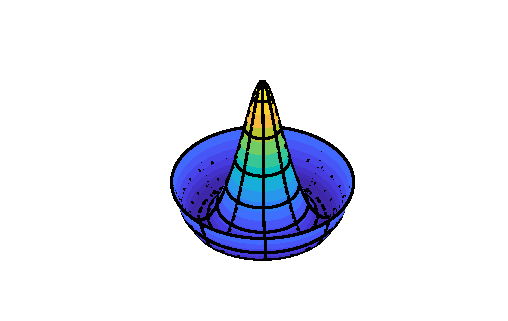
\includegraphics[scale=3]{CouvPot.pdf}
\end{center}
\label{fig:Intro}
\end{figure}


\vfill
\hfill

\includegraphics[scale=0.25]{parisSaclay.jpg}
\pagebreak

%\vspace*{4pt}
\end{titlepage}
\pagebreak

\strut
 \thispagestyle{empty}
\newpage






% On commence le compteur de page ici
 \setcounter{page}{1}

\begin{flushleft}
\color{bleu}
{\fontsize{14}{14} \selectfont
	\textbf{Remerciement}}\\

\color{black}
\end{flushleft}

Je souhaiterais remercier l'ensemble des membres du LPTMC que j'ai eu le plaisir de rencontrer pour leur accueil chaleureux. Je remercie tout particulièrement Bertrand Delamotte et Nicolas Dupuis pour leur encadrement et toute l'aide qu'ils m'ont apportée.

\vspace*{11pt}

\begin{flushleft}
\color{bleu}
{\fontsize{14}{14} \selectfont
	\textbf{Acknowledgments}}\\

\color{black}
\end{flushleft}

I would like to thank all the members of LPTMC whom I had the pleasure to meet for their warm welcome. I wish to express my particular thanks to Bertrand Delamotte and Nicolas Dupuis for their supervision, their advice and their help.
\vspace*{22pt}





\begin{center}
\rule{13.7cm}{.5pt}
\end{center}

\vspace*{-11pt}
\begin{abstract}
Nous étudions dans différents systèmes les transitions de phase produites par un changement de température $T$. Dans un système donné une transition de phase se produit pour une température dite critique $T_c$ et provoque des changements de ses propriétés physico-chimiques. Les grandeurs thermodynamiques qui le caractérisent deviennent des fonctions qui s'expriment en puissance de $T-T_c$, singulières en $T=T_c$. On peut définir des nombres réels, appelés \textit{exposants critiques}, qui caractérisent ces singularités. Ils ont la particularité d'être identiques pour deux milieux différents du moment que ces derniers partagent des propriétés de symétries communes. Le formalisme du groupe de renormalisation non perturbatif (NPRG) doit permettre de calculer numériquement ces exposants et $T_c$ à travers la résolution d'équations integro-différentielles non linéaires : les équations "BMW". Le calcul de $T_c$ de systèmes complexes reste cependant difficile avec cette approche. Notre but général est d'établir des simulations de résolution de ces équations pour vérifier la faisabilité et la précision des calculs. \\
\indent
Dans un premier temps notre objectif a été d'essayer de corriger un premier code de simulation de ces équations pour une première classe de systèmes (possédant la symétrie $O(N)$. Ce code présentait des irrégularités et des instabilités dans certaines configurations. Malgré tous nos efforts, les problèmes numériques subsistent encore, même si nous pensons en avoir cerné au moins une des causes. Dans un second temps nous avons écrit un nouveau code qui nous a permis de calculer numériquement $T_c$ pour le modèle dit \textit{d'Ising 2D}, avec une simulation des équations BMW. Nous avons pu la comparer à la valeur théorique attendue. Nous avons pour cela dû tester différentes méthodes numériques. Nous obtenons une erreur de $\sim 4 \%$. Cet écart reste plus élevé que ce qui été espéré mais il n'est pas particulièrement fiable à cause d'imprécisions de calcul observables dans les solutions numériques obtenues.
\end{abstract}

\begin{center}
\rule{8cm}{.5pt}
\end{center}


\renewcommand{\abstractname}{Abstract}
\begin{abstract}

We study second order phase transitions produced by temperature variations. In a given system a phase transition occurs at a given temperature said to be the critical temperature et causes changes in its physical and chemical properties. Its thermodynamical quantities appear to scale as power laws of $T-T_c$ and they have a singularity in $T=T_c$. This singularities are characterized with real numbers called the \textit{critical exponents} that have the interesting peculiarity of being universal for all systems sharing the same properties of symmetry. In the framework of the non perturbative renormalisation group it is possible to compute numerically these exponents as well as $T_c$ thanks to the resolution of non linear partial differential equations : the BMW equations. It is well known that computing $T_c$ for complex system is difficult within this framework. Our general goal is to write numerical simulations to solve the BMW equations and check if they give the expected results with a satisfying accuracy. \\
\indent
In a first part we tried to fix a simulation code which computed the critical exponents (for systems with the symmetry $O(N)$). This code had problems in several configurations. Unfortunately there are still numerical problems today even though we believe that we found what causes at least one of them. In a second part we wrote a new code to compute $T_c$ for the complex \textit{Ising 2D} model thanks to numerical resolution of the BMW equations. We were able to compare our result to the theoretical value expected. We tested several numerical methods and we found an error of $4 \%$. This difference is higher than what was expected but it is not entirely reliable since the simulation shows irregularities and a certain inaccuracy that we could not overcome.
\end{abstract}


\begin{center}
\rule{13.7cm}{.5pt}
\end{center}

\pagebreak 

\tableofcontents

\pagebreak
\begin{multicols*}{2}

\section{Introduction}


La physique statistique établit un cadre permettant de calculer les grandeurs macroscopiques, dites aussi thermodynamiques, des problèmes mettant en jeu des systèmes avec un très grand nombre de degrés de liberté en interaction. Pour donner une image de ce que cela signifie, on considère un litre d'eau enfermé dans une boite. Ce litre d'eau est constitué de $\sim 10^{24}$ molécules qui possèdent toutes plusieurs degrés de liberté chacune : leur position, leur vitesse etc. On remarque alors que, un seul litre d'eau, possède un nombre colossal de degrés de liberté qui peuvent interagir ensembles (par l'intermédiaire, entre autre, des collisions des molécules). Il n'est donc pas possible de déterminer les propriétés physiques macroscopiques de ce système en étudiant la dynamique individuelle de chaque degré de liberté le constituant, ce pourquoi on a recours à la physique statistique. 

Nous allons nous intéresser ici plus particulièrement à un domaine particulier de la physique statistique et de la thermodynamique qu'est l'étude des transitions de phase. Nous commençons par décrire un exemple plus précis de système aux degrés de liberté en interactions, le système d'Ising 2D, nous permettant d'introduire la notion de phase et de transition de phase. Enfin nous expliciterons ce que que nous avons plus particulièrement étudié dans ces phénomènes et comment nous nous y sommes pris. \\




\subsection{Le modèle d'Ising 2D}


\label{sec:IsingIntro}

Pour donner une image concrète d'un système aux degrés de liberté en interaction nous introduisons le système le plus simple à appréhender que l'on appelle le modèle d'Ising à deux dimensions et qui permet de décrire certains matériaux aimantés. \\

On se place dans l'espace à trois dimensions repéré par la base unitaire cartésienne $\{\ev_\nu\}_{\nu=x,y,z}$ de $\R^3$. On considère un réseau carré de pas $a$ dans le plan $(\ev_x, \ev_y)$. Soit $L \in \N^*$, on note $\mathscr{R} = \left\{ m a \ev_x + n a \ev_y \, | \, (m, n) \in  \bbrac{0,L}^2 \right\}$ l'ensemble des positions des noeuds du réseau dans la surface $[0, aL]^2$.  

Sur chaque noeud dans  $[0, aL]^2$ se trouve un spin à une composante qui se représente par un vecteur dont la direction est parallèle à $\ev_z$ et dont l'orientation peut être selon $+\ev_z$ ou $-\ev_z$. Pour représenter le sens du spin à la position $\rv \in \mathscr{R}$, on lui associe le scalaire $S_\rv$ qui vaut $+1$ s'il est selon $+\ev_z$ et $-1$ s'il est selon $-\ev_z$, ce sont les degrés de liberté du système. Dans un modèle cohérent de la réalité nous avons un nombre $N_s = (L+1)^2 \sim 10^{24}$ de spins, autant dire un nombre "quasi-infini". 

On appelle \textit{micro-état} ou \textit{configuration} du système un ensemble $\Mr = \{ S_\rv \}_{\rv \in \mathscr{R}}$ donné : par exemple $\Mr = \{ S_0 = 1, S_{a\ev_x} = -1, S_{a\ev_y} = 1, S_{a\ev_x + a\ev_y} = 1, ...\}$ est un micro-état. Une représentation en terme de vecteurs en est faite en \refig{schemaIsing}. Il existe alors $2^{N_s} \sim 2^{10^{24}}$ micro-états possibles différents. Dans le modèle d'Ising, pour un micro état $\Mr$ on peut définir son énergie associée à l'aide du \textit{hamiltonien}, $H(\Mr)$ défini par 
\begin{equation}
H\(\Mr = \{ S_\rv \}_{\rv \in \mathscr{R}} \) = -J \sum_{\left<\rv, \rv'\right>}S_\rv S_{\rv'} \, .
\label{eq:HamIsing}
\end{equation}
La notation $\left<\rv, \rv'\right>$ signifie que l'on somme sur tout $\rv \in \mathscr{R}$ et $\rv' \in \mathscr{R}$  mais que le terme $S_\rv S_{\rv'}$ contribue à la somme si et seulement les noeuds $\rv$ et $\rv'$ sont plus proches voisins (i.e si $\rv' = \rv \pm a \ev_x$ ou $\rv' = \rv \pm a \ev_y$). On remarque alors que les spins interagissent ensemble. Le paramètre $J$ représente une énergie, c'est une constante positive.\\

Supposons maintenant que le système soit soumis à un champ magnétique extérieur $\bv$ stationnaire. Ce champ peut prendre une valeur différente pour chaque noeud. On note $b_\rv \ev_z$ sa valeur au noeud $\rv$ ainsi que  $\mathcal{B} = \{b_\rv\}_{\rv \in \Rr}$. L'énergie du micro-état $\Mr$ s'en trouve alors changée et elle est décrite par un nouvel hamiltonien :
\begin{equation}
	\mathcal{\Hc}(\Mr, \mathcal{B}) = H(\Mr) - \sum_\rv b_\rv S_\rv \, ,
\end{equation}
La somme sur $\rv$ est une somme sur l'ensemble des $N_s$ positions des spins dans le réseau.
\setlength{\unitlength}{1cm}
\begin{figure}[H]
\begin{center}
\begin{picture}(6,3.8)

\put(-0.5,2.6){\vector(0,1){0.8}}
\put(-0.5,2.6){\vector(1,0){0.8}}
\put(-0.5,2.6){\vector(1,3){0.2}}
\put(-1, 2.95){$\ev_z$}
\put(-0.3, 2.25){$\ev_x$}
\put(-0.2, 3.0){$\ev_y$}

\color{cyan}
\put(0,0){\line(1,3){1.2}}
\put(1,0){\line(1,3){1.2}}
\put(2,0){\line(1,3){1.2}}
\put(3,0){\line(1,3){1.2}}
\put(4,0){\line(1,3){1.2}}
\put(5,0){\line(1,3){1.2}}

\put(-0.25,0.45){\line(1,0){5.7}}
\put(0.05,1.25){\line(1,0){5.7}}
\put(0.25,2.0){\line(1,0){5.7}}
\put(0.45,2.70){\line(1,0){5.7}}
\put(0.65,3.35){\line(1,0){5.7}}
\color{red}
\linethickness{0.35mm}

\put(0.15,0.85){\vector(0,-1){0.8}}
\put(1.15,0.05){\vector(0,1){0.8}}
\put(2.15,0.85){\vector(0,-1){0.8}}
\put(3.15,0.05){\vector(0,1){0.8}}
\put(4.15,0.05){\vector(0,1){0.8}}
\put(5.15,0.85){\vector(0,-1){0.8}}

\put(0.4167,1.6){\vector(0,-1){0.7}}
\put(1.4167,0.9){\vector(0,1){0.7}}
\put(2.4167,0.9){\vector(0,1){0.7}}
\put(3.4167,0.9){\vector(0,1){0.7}}
\put(4.4167,1.6){\vector(0,-1){0.7}}
\put(5.4167,0.9){\vector(0,1){0.7}}

\put(0.667,1.7){\vector(0,1){0.6}}
\put(1.667,1.7){\vector(0,1){0.6}}
\put(2.667,2.3){\vector(0,-1){0.6}}
\put(3.667,1.7){\vector(0,1){0.6}}
\put(4.667,1.7){\vector(0,1){0.6}}
\put(5.667,1.7){\vector(0,1){0.6}}

\put(0.9,2.45){\vector(0,1){0.5}}
\put(1.9,2.95){\vector(0,-1){0.5}}
\put(2.9,2.45){\vector(0,1){0.5}}
\put(3.9,2.45){\vector(0,1){0.5}}
\put(4.9,2.95){\vector(0,-1){0.5}}
\put(5.9,2.45){\vector(0,1){0.5}}

\put(1.1167,3.55){\vector(0,-1){0.4}}
\put(2.1167,3.15){\vector(0,1){0.4}}
\put(3.1167,3.15){\vector(0,1){0.4}}
\put(4.1167,3.55){\vector(0,-1){0.4}}
\put(5.1167,3.55){\vector(0,-1){0.4}}
\put(6.1167,3.15){\vector(0,1){0.4}}

\end{picture}
\end{center}
\vspace*{-11pt}
\caption{Exemple de micro-état possible du réseau d'Ising tronqué ou seuls quelques vecteurs sont représentés. Leur direction est fixe selon l'axe $\ev_z$ mais ils peuvent avoir un sens différent.}
	\label{fig:schemaIsing}
\end{figure}

A température nulle et sans champ magnétique extérieur ($\mathcal{B} = 0$) le système ne peut se trouver que dans les configurations minimisant son énergie H.  Comme $J$ est positif ceci se produit pour $\Mr_1 = \{1,1,1 .., 1\}$ ou $\Mr_{-1} = \{-1,-1,-1 .., -1\}$, micro-états dans lesquels l'ensemble des spins sont tous orientés dans la même direction. Le système à une chance sur deux de se trouver dans $\Mr_1$ et une chance sur deux dans $\Mr_{-1}$.

\commentout{
A température nulle et sans champ magnétique extérieur ($\mathcal{B} = 0$) le système va se trouver dans les configurations minimisant son énergie 
Si le système est placé dans un milieu à température nulle, sans champ magnétique extérieur ($\mathcal{B} = 0$), et initialement dans un micro-état quelconque il évolue vers le micro-état minimisant son énergie, donc minimisant $H$. Comme $J$ est positif ceci se produit pour $\Mr_1 = \{1,1,1 .., 1\}$ ou $\Mr_{-1} = \{-1,-1,-1 .., -1\}$, micro-états dans lesquels l'ensemble des spins sont tous orientés dans la même direction. En effet, dans le micro état $\Mr_1$ par exemple nous avons $S_\rv S_{\rv'} = 1$ pour tout site en $\rv$ et $\rv'$ dans $\mathscr{R}$ plus proches voisins et $H$ est alors bien minimisé. Ceci permet aussi aussi de montrer ce qu'un système aux degrés de liberté en interaction représente. En effet considérons le système dans le micro-état $\Mr_1$ et imagions que l'on puisse tourner un spin, i.e. imposer $S_\rv=-1$ pour un $\rv$ donné. Alors, pour minimiser l'énergie, par la forme du hamiltonien, ses quatre spins plus proches voisins vont  interagir avec lui  et le "contraindre" à revenir dans la position $S_\rv = 1$. \\}

Lorsqu'il est soumis à une température $T$ non nulle, le système reçoit de l'énergie thermique de l'extérieur qui tend à favoriser la désorganisation des spins : son état d'équilibre n'est plus un micro-état particulier. En revanche, en présence d'un champ magnétique extérieur on peut définir la probabilité qu'à l'équilibre le système soit dans le micro-état $\Mr$ par
\begin{equation}
	p\(\Mr, T, \mathcal{B}, N_s\) = \frac{1}{\Zc(T, \mathcal{B}, N_s)}\exp\(-\frac{\Hc\(\Mr, \Bc\)}{k_B T} \)
\end{equation}
avec la notation
\begin{equation}
\Zc(T, \mathcal{B}, N_s) = \sum_{\Mr'}  \exp\(-\frac{\mathcal{\Hc}\(\Mr', \Bc\)}{k_B T} \) \, . 
\end{equation}
La fonction $\Zc(T, \Bc)$ est appelée la fonction de partition du système, il s'agit d'une somme sur l'ensemble  des $2^{N_s}$ micro-états possibles. La constante $k_B$ est la constante de Boltzmann. 

 Plus la température est élevée plus l'énergie thermique reçue que l'on peut évaluer par $\sim k_BT$ est grande par rapport à l'énergie $J$. Si l'on raisonne à champ magnétique extérieur nul ($\Bc= 0$), pour $k_BT \ll J$ les probabilités sont telles que le systèmes ne peut se trouver que dans $\Mr_1$, $\Mr_{-1}$ ou des micro-états proches de $\Mr_1$ ou $\Mr_{-1}$. En revanche, lorsque $k_BT \gg J$ les spins reçoivent suffisamment d'énergie thermique pour que le système puisse être indifféremment dans n'importe quel micro-état à l'équilibre. \\




L'ensemble des grandeurs du système sont calculées comme des moyennes statistiques sur les différents micro-états. 
En particulier une des grandeurs caractéristique du système est son aimantation moyenne. En effet, comme nous l'avons mentionné le modèle d'Ising décrit la physique des matériaux aimantés. Les spins agissent comme de petits aimants individuels et l'aimantation totale correspond donc à la somme des spins. Ainsi l'aimantation du micro-état $\Mr  = \{ S_\rv \}_{\rv \in \mathscr{R}}$ est
\begin{equation}
	m_\Mr(N_s) = \frac{1}{N_s} \sum_{\rv} S_\rv \, .
\end{equation}
En utilisant la description statistique il est alors possible de déterminer l'aimantation $m$ totale (i.e. macroscopique), que possèderait un matériau décrit par le modèle d'Ising à une température $T$ donnée, selon les formules
\begin{equation}
	\begin{split}
	m(T, \Bc, N_s)  &  \equiv \left< m_\Mr(N_s) \right>	\, , \\
	 & \equiv \sum_{\Mr} p\(\Mr, T, \Bc, N_s \) \(\frac{1}{N_s} \sum_{\rv} S_\rv\)  \, .
	\end{split}
\end{equation}
On montre que $m$ se ré-exprime aussi selon 
\begin{equation}
	m(T, \Bc, N_s) = \frac{1}{N_s\beta}\partial_\beta \ln\(\Zc(T, \Bc, N_s) \) 
\end{equation}
avec $\beta = 1/(k_BT)$. Nous en reparlerons plus loin mais de manière générale la fonction de partition $\Zc$ à une importance particulière car elle permet comme ici avec $m$ de retrouver toutes les grandeurs macroscopiques intéressantes du système que l'on étudie. \\

Nous nous intéressons à l'aimantation à champ magnétique extérieur uniforme $\Bc = \{b_\rv = b\}_\rv$ car elle va nous permettre d'introduire le concept de transition de phase. En effet, nous pouvons remarquer que pour $N_s$ et $T$ donnés $m$ est une fonction impaire du champ magnétique, $m(T, -b, N_s) = m(T, b, N_s)$. Ceci est dû à l'invariance de $H$ pour le changement de $\ev_z$ en $-\ev_z$ : $H(\{-S_\rv\}) = H(\{S_\rv\})$. Ainsi, $m(T, b=0, N_s) = 0$, l'aimantation est nulle quand le champ magnétique extérieur est nul. Cependant pour décrire l'aimantation d'un système réel il faut d'abord calculer $m$ dans limite $N_s \to \infty$ (on suppose que cela est possible), que l'on appelle limite thermodynamique. On montre qu'il apparait alors une singularité. Pour $T$ inférieur à une certaine valeur, notée $T_c$, 
\begin{equation}
	\lim_{b\to 0} \lim_{N_s\to \infty} m(T,b,N_s) =
	\begin{cases}
			> 0 & \text{si} \quad b \to 0^+ \\
			< 0 & \text{si} \quad b  \to 0^- \, .
	\end{cases}
\end{equation}
Dans un système réel le champ magnétique extérieur n'est jamais complètement nul, avoir $b = 0^+$ ou $b=0^-$ donne des aimantations opposées. Cet effet se nomme la brisure spontanée de symétrie : le caractère impair de $m$ par rapport à $b$, dû à la symétrie de $H$ est perdu. Notons $m(T, b)= \lim_{N_s \to \infty} m(T,b,N_s)$.
\begin{figure}[H]
\begin{center}
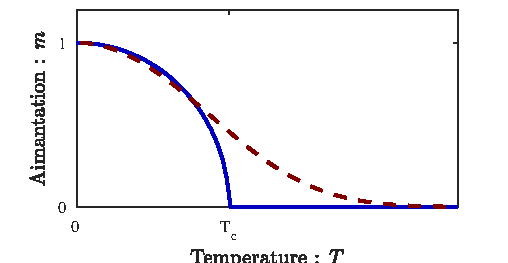
\includegraphics[width=0.95\columnwidth]{aimantation.pdf}
\caption{Evolution de l'aimantation $m$ du système en fonction la température à champ magnétique extérieur uniforme $b = 0^+$ et dans la limite thermodynamique (bleu continu). Même chose pour $b = 0^-$ (rouge pointillée).}
\label{fig:aimantation}
\end{center}
\end{figure} 
\vspace*{-11pt}
Il est possible de tracer l'évolution de $m$, dans la limite $N_s \to \infty$ pour $b \simeq 0$ en fonction de $T$ (numériquement ou expérimentalement sur des systèmes décrits par le modèle d'Ising 2D). On obtient alors les courbes de \refig{aimantation} ayant une cassure au niveau de la température $T_c$.  Un système décrit par ce modèle, placé dans un milieu sans champ magnétique, est aimanté pour $T<T_c$ mais perd son aimantation pour $T>T_c$. Si l'on introduit l'énergie libre
\begin{equation}
F(T, \Bc, N_s) = -\ln(\Zc(T, \Bc, N_s))\, ,	
\end{equation}
alors la cassure est liée à la présence d'une singularité de 
\begin{equation}
f(T, \Bc) = \lim_{N_s \to \infty} \frac{F(\Bc, N_s)}{N_s}
\end{equation} 
en $T=T_c$.
Cette évolution caractéristique de $m$ marque la présence d'une transition de phase. Pour bien comprendre  ce dont il s'agit définissons ce qu'est, de manière générale, une transition de phase et comment les étudier. \\









\subsection{Transitions de phase}
\subsubsection{Définition et classification}

En thermodynamique on note $F$ l'énergie libre d'un système. C'est une fonction caractéristique du système qui dépend de son volume et de différents paramètres comme la température $T$ extérieure, le champ magnétique extérieur, etc. On appelle alors phase une région de l'espace des paramètres où $f : (T, ...) \to \lim_{V \to \infty} F(V,T...)/V$ est analytique (en supposant que cette limite, appelée limite thermodynamique, existe). En faisant varier les paramètres de $f$ il est possible de passer d'une zone d'analyticité à une autre en passant alors par des points singuliers de $f$ : le système subit une transition de phase. Les paramètres pour lesquels $f$ est singulière sont appelés les paramètres critiques. On ne s'intéressera ici qu'à l'influence de la température avec tous les autres paramètres fixés. On notera alors $T_c$ la température critique. Dans les faits un changement de phase est dû à une réorganisation, au niveau microscopique, des constituants  du système (molécules, atomes, spins ...), ayant un effet macroscopique. Landau a classé ces transitions suivant deux types : celles du premier ordre et celles du second \cite{toledano1987landau}. La distinction se fonde sur la continuité d'une fonction que l'on appelle le paramètre d'ordre, au moment de la transition. 
 \begin{figure}[H]
\begin{center}
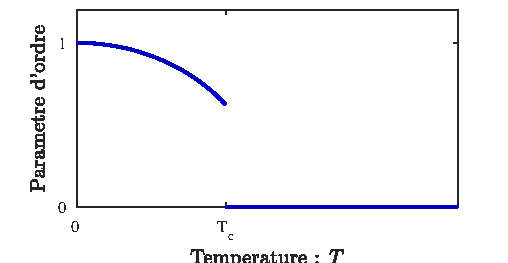
\includegraphics[width=0.95\columnwidth]{aimantation2.pdf}
\caption{Exemple d'évolution du paramètre d'ordre pour une transition de phase du premier ordre}
\label{fig:aimantation2}
\end{center}
\end{figure}
\vspace*{-11pt}
Dans l'exemple du modèle d'Ising 2D, avec un champ magnétique extérieur uniforme $\bv = b\ev_z$, nous avons vu que $F$ dépend de $V$ (puisque $V$ est donné par $V = a^2 N_s$), de $T$ et de $b$. Il existe $T_c$ tel que $(T,b) \to f(T,b)$ soit singulière en $T$ = $T_c$. La température permet de réorganiser la structure microscopique du modèle en modifiant la "quantité de désordre" des spins. A champ magnétique extérieur $b = 0^+$ ou $b = 0^-$ et à $T< T_c$, ils ont tendance à rester alignés et ordonnés dans une direction privilégiée c'est une phase. En revanche pour $T>T_c$ les spins ont un comportement désordonné, c'est une seconde phase. L'aimantation correspond au paramètre d'ordre de la transition. C'est une fonction continue avec la température : il s'agit donc d'une transition du second ordre. Une transition du premier ordre\footnote{Le passage de l'eau de l'état liquide à l'état gazeux par augmentation de la température à pression constante en est un exemple.} aurait eu un paramètre d'ordre évoluant comme la courbe de \refig{aimantation2}.  


\subsubsection{Transitions du second ordre : définition des exposants critiques, universalité}

Il se produit, lors des transitions du second ordre, des phénomènes particuliers, qui sont au centre de l'étude que nous avons réalisé. Pour les expliquer introduisons, pour tout système, une fonction de corrélation\footnote{ Il est possible de déterminer expérimentalement \cite{Bellac2012} cette fonction.} $G^{(2)}(r)$ qui décrit quantitativement l'influence que deux degrés de liberté séparés d'une distance $r$ ont l'un sur l'autre.. Notons que plus $r$ sera grand moins cette influence sera forte et donc plus $G^{(2)}(r)$ sera faible. 

Dans le cas du modèle d'Ising cette fonction représente l'influence que deux spins $S_{\rv_1}$ et $S_{\rv_2}$ ont l'un sur l'autre à $T$ et $\Bc = \{b_\rv\}_\rv$ fixés. Elle est plus exactement définie, par
\begin{equation}
\begin{split}
	G^{(2)}(|\rv_1 - \rv_2|) & \equiv \left< S_{\rv_1} S_{\rv_2} \right> \\
	&  \equiv \sum_{\Mr}  p\(\Mr, T, \Bc, N_s\) S_{\rv_1} S_{\rv_2} \, 
	\end{split}
\end{equation}
et elle se calcule aussi directement en utilisant la fonction de partition avec l'expression 
\begin{equation}
	G^{(2)}(|\rv_1 - \rv_2|) = \frac{1}{\Zc(T, \Bc, N_s)} \frac{\partial^2 \Zc(T, \Bc, N_s)}{\partial b_{\rv_1} \partial b_{\rv_2}} \, .
\end{equation}

On appelle $\xi$, longueur de corrélation, la distance approximative à partir de laquelle deux degrés de libertés du système n'ont plus d'influence l'un sur l'autre. On observe alors expérimentalement que de manière générale, dans la limite thermodynamique, pour toute transition de phase du second ordre les grandeurs $\xi$ et $G^{(2)}$ évoluent selon 
\begin{equation}
	\xi \widesim{T \to T_c} |T-T_c|^{-\nu}
\end{equation}
et, pour $T = T_c$,
\begin{equation}
	 G^{(2)}(r) \widesim{r \to \infty} |r|^{2-d-\eta},
\end{equation}
où $d$ est la dimension physique du système ($d=2$ pour Ising 2D) et $\nu$ et $\eta$ sont deux réels positifs appelés les \emph{exposants critiques}.  Il apparait que deux systèmes différents, définis dans une même dimension $d$, mais qui possèdent des propriétés de symétries communes, ont les mêmes exposants critiques. Dans le modèle d'Ising 2D, nous avons déjà mentionné que l'échange de $\ev_z$ en $-\ev_z$ ne change pas l'hamiltonien du système, on dit alors qu'il possède une symétrie $\mathbb{Z}_2$. Pour tout système à $d=2$ ayant la même propriété et défini sur le même réseau nous obtiendrons donc un $\eta$ et un $\nu$ identiques. Nous détaillons plus tard, en \refsec{ON}, ce qu'est la symétrie $O(N)$  à laquelle nous nous sommes intéressés. \\


\subsubsection{Objectif général : importance de la fonction de partition}

Dans les grandes lignes, le but de notre étude est de calculer les exposants critiques $\nu$ et $\eta$ ainsi que la température critique $T_c$ pour différents systèmes possédant la symétrie $O(N)$ et une transition de phase du second ordre. Sur tous les systèmes étudiés il est possible de définir une fonction de partition $\Zc$ qui possède un rôle fondamental dans l'étude des transitions de phase. En effet, pour un système donné elle permet de déterminer toute les grandeurs macroscopiques qui y sont rattachées. Dans le modèle d'Ising 2D nous avons montré par exemple qu'elle permet de calculer l'aimantation $m$ et la fonction de corrélation à deux points $G^{(2)}$. Or c'est la connaissance de $G^{(2)}$ qui définit les exposants critiques $\eta$ et $\nu$.\\

Il s'avère cependant qu'il n'est pas toujours possible de calculer la fonction de partition d'un système de manière exacte. Dans la grande majorité des cas cela est même impossible. On utilise alors des méthodes de calculs approchées. Le modèle d'Ising 2D est un exemple de cas particulier où la fonction de partition peut être calculée exactement, ceci a été fait par Onsager \cite{Onsager}. \\

Nous avons utilisé dans cette étude une méthode de calcul numérique approchée des fonctions de partition en utilisant les outils du groupe de renormalisation. Nous détaillerons ces méthodes en \refsec{RG}. Cela nécessite cependant d'étudier des systèmes qui ne sont pas décrit par des ensembles de valeurs discrètes (i.e. $\{S_\rv\}_\rv$ dans le cas du modèle d'Ising 2D), mais par des champs. Nous introduisons donc les concepts fondamentaux de mécanique statistique des champs. \\




\subsection{Formalisme de mécanique statistique des champs}

\label{sec:Origin}

\subsubsection{La notion de champ}

Nous introduisons brièvement dans cette sections le formalisme de la physique statistique \cite{diu2007thermodynamique} des champs. Ceci est nécessaire pour pouvoir aborder l'étude des transitions de phase et des exposants critiques à l'aide de l'outil du groupe de renormalisation (RG). \\

Considérons un système à $P$ corps (atomes, molécules, spins  ...) dans un ouvert à $d$ dimensions $\Omega$ de volume $|\Omega|$. On suppose que chacun de ces $P$ corps possède $N$ degrés de liberté. Dans le modèle d'Ising 2D, $d=2$, $P=N_s$, $\Omega = ]0, aL[^2$ où $a$ est le pas du réseau et $N=1$. En effet on ne dispose que d'un degré de liberté par spin dans le sens ou une seule variable scalaire $S_\rv$ pour le spin à la position $\rv$ suffit pour décrire le système. Un modèle équivalent avec $N=2$ serait un modèle avec des spins à deux composantes sur chaque noeud nécessitant d'être représentés par deux variables scalaires. \\

On introduit maintenant une fonction $\varphiv$ définie par
\begin{equation}
 \varphiv \in \( \Cc^{0}(\Omega)\)^N : \rv \in \Omega \rightarrow \varphiv(\rv) \in \R^N \, ,
\end{equation}
normalisée, et on suppose que $\varphiv$ décrit, au même titre que l'ensemble $\Mr = \{S_\rv\}_\rv$ dans le modèle d'Ising, une configuration du système. On l'appelle alors le \textit{champ} du système. L'hamiltonien devient de façon équivalent une fonctionnelle de $\varphiv$, on le note $H[\varphiv]$. Il représente l'énergie du système dans la configuration du champ $\varphiv$. Si un champ magnétique externe défini par $\bv : \rv \to \bv(\rv) \in \R^N$ agit sur le système alors on introduit l'hamiltonien $\Hc$ dépendant de $\bv$ par
\begin{equation}
	\Hc[\varphiv, \bv] \equiv H[\varphiv] -  \int_{\Omega} \bv(\rv) \varphiv(\rv) \, \dd \, \rv  \, .
\end{equation}
Avec le formalisme canonique de la physique statistique \cite{rohtuA} nous savons que nous pouvons connaitre toutes l'information sur les propriétés macroscopiques du système soumis à une température $T$ et champ magnétique $\bv$ en étudiant sa fonction de partition $\Zc$ définie par l'expression 
\begin{equation}
\Zc[T; \bv] \equiv \int \Dc \varphiv \, \exp\(- \frac{\mathcal{H}[\varphiv, \bv]}{k_BT}\) \, . 
\end{equation} 
Cette intégrale avec une notation $\Dc \varphiv$ est une intégrale dite \textit{fonctionnelle} sur l'ensemble des champs $\varphiv$ pouvant décrire le système. C'est donc une somme sur un ensemble continu de fonctions ; une somme "continue" équivalente à la somme sur tous les $\Mr$ micro-états possibles. Elle ne peut être calculée de façon exacte que pour quelques hamiltoniens très particuliers. Comme nous l'avons déjà mentionné un calcul approché peut en être fait par le groupe de renormalisation. 


\subsubsection{Un exemple : le modèle $\varphiv^4$}


\label{sec:modphi4}

Pour illustrer ce que l'on vient d'introduire sur la théorie des champs et sur les transitions de phases nous pouvons nous intéresser à l'exemple du système défini par l'hamiltonien de la théorie $\varphiv^4$. Cet hamiltonien est
\begin{equation}
		H[\varphiv] = \int_\Omega \, \left\{ \frac{1}{2}(\nabla\varphiv)^2 + \frac{1}{2}r_0 \varphiv^2 + \frac{u_0}{4!}{\({\varphiv}^{2}\)}^{2} \right\} \, .
		\label{eq:hamiltCont}
\end{equation}
Nous avons intégré dans son expression le terme $k_BT$ pour avoir une expression plus simple. Plus précisément, la fonction de partition associée s'écrit, à champ magnétique extérieur nul $\bv =0$, 
\begin{equation}
		\Zc[T] = \int \Dc \varphiv \, \exp\( - H[\varphiv]\) \, ,
\end{equation}
et $r_0 = \bar{r}_0(T-T_0)$ avec $T$ la température à laquelle est soumise le système, $T_0$ une température caractéristique du système et $\bar{r}_0$, $u_0$ deux réels définis par le système. \\

Si $u_0=0$ alors l'intégrale définissant $\Zc$ est \textit{gaussienne} et il est possible de la calculer, c'est un rare cas où cela est possible. Pour un tel système on peut alors montrer que $T_c = T_0$ et pour $T = T_0 = T_c$
\begin{equation}
	G^{(2)} (r) \widesim{r \to \infty} |r|^{2-d} \, .
\end{equation}
De plus il vient aussi
\begin{equation}
	\xi \widesim{T \to T_0} |T - T_0|^{-\frac{1}{2}} \, .
\end{equation}
Ainsi, dans ce cas là, $\eta = 0$ et $\nu = 1/2$.\\ 

Si $u_0 \neq 0$ alors les choses sont plus compliquées, l'intégrale ne peut plus être calculée de manière exacte, $T \neq T_0$, $\nu \neq 1/2$ et $\eta  > 0$. En revanche la propriété d'universalité de ces exposants critiques est valable. Un système ayant des symétries identiques au système d'écrit par l'hamiltonien $\varphiv^4$ avec $u_0 \neq 0$ possèdera les mêmes exposants critiques. Si jamais $d \ge 4$, pour déterminer $\eta$, $\nu$ et $T_c$ il suffit de faire un calcul approché en développant l'expression de $\Zc$ en puissances de $u_0$, cependant si $d < 4$ nous avons besoin d'autres méthodes d'approximations pour calculer $\Zc$. Le groupe de renormalisation en est une.\\


\subsection{Intérêt de l'approche par la théorie statistique des champs. Intérêt du RG et du NPRG}


Le formalisme de théorie des champs consiste à travailler avec des fonctions continues appelées \textit{champs} et non plus des ensembles de variables à valeurs discrètes (comme les micro-états du modèle d'Ising 2D). Il ne permet donc pas de décrire le modèle d'Ising 2D, a priori. En revanche il est utile car il permet de réaliser des calculs plus facilement. Si un système dont l'état est défini par des champs possède les mêmes symétries qu'un autre système quelconque (pas forcément décrit par des champs), alors ils ont les mêmes exposants critiques. Le calcul des exposants critiques en théorie des champs par le RG, à travers le calcul de la fonction de partition, s'applique à tous les systèmes possédant la même symétrie. Introduisons donc le RG, le NPRG ainsi que ce qu'il permettent. \\

Comme nous venons de le mentionner le groupe de renormalisation (RG) permet de calculer, avec des approximations controlées, les fonctions de partition $\Zc$ définies à l'aide de champs. Cette méthode a permis de calculer différents exposants critiques pour différents systèmes. Les calculs ont donné d'excellents résultats \cite{kadanoff1967scaling, wilson1971renormalization2} par rapports à ce qui avait pu être obtenu par expérience ou par d'autres méthodes comme les simulations Monte-Carlo. C'est une méthode qui permet aussi d'expliquer pourquoi les exposants critiques sont identiques au sein d'une même classe d'universalité (une classe d'universalité étant l'ensemble des systèmes possédant les même propriétés de symétrie). \\
\indent
Cependant elle reste limitée dans ces applications car elle utilise des approximations relativement importantes. En effet, la température critique $T_c$ est une grandeur qui n'est pas universelle, deux systèmes différents ayant beau avoir les mêmes propriétés de symétrie ont deux températures critiques différentes. Les approximations faites par le RG sont suffisantes pour étudier des systèmes simples possédant les symétries de systèmes plus complexes que l'on souhaite étudier (ce qui suffit par l'effet d'universalité pour calculer les exposants critiques) mais elle ne sont pas assez précises pour calculer directement $T_c$ sur ces modèles complexes .\\

Le groupe de renormalisation non perturbatif (NPRG) est une extension du RG qui peut répondre à ce problème en reprenant le même principe sous une approche différente. On détermine $\Zc$ grâce à des équations solubles numériquement en utilisant l'approximation dite \textit{BMW} (Blaizot - Méndez-Galain - Wschebor) \cite{Blaizot}. Cela permet plus de précision et de flexibilité que les approximations faites dans le RG. De plus, elle permet, a priori, de calculer des grandeurs comme $T_c$ sur des systèmes complexes. Nous en avons étudié l'efficacité dans notre étude. Nous aborderons plus en détails les principes du RG, du NPRG et de l'approximation BMW en \refsec{RGGeneral}. Introduisons maintenant brièvement la symétrie $O(N)$ avant d'aborder les objectifs précis de notre étude.


\subsection{Les systèmes à symétrie $O(N)$}

\label{sec:ON}

Le but est d'étudier les exposants critiques des systèmes possédant un symétrie $O(N)$. Nous pouvons définir ceci assez simplement maintenant que nous avons introduit le formalisme de physique statistique des champs. \\
 
On dit qu'un système est symétrique selon $O(N)$ pour $N \ge2 $ si son hamiltonien est invariant par l'action du groupe de rotation $O(N)$ sur ces degrés de libertés. Dans le cas où $N=1$ on fera référence à la symétrie $\mathbb{Z}_2$ qui est équivalente. Par exemple, dans le formalisme de la théorie des champs, soit $J \in O(N)$, et on note $J.V$ l'action de $J$ sur un vecteur $V$ de $\R^N$. Le modèle est dit invariant sous $O(N)$ si 
\begin{equation}
	H[J .\varphiv] = H[\varphiv]	 
\end{equation}
et il est dit invariant sous $\mathbb{Z}_2$ si $H[-\varphi] = H[\varphi]$. Le modèle d'Ising 2D est aussi un modèle invariant sous $\mathbb{Z}_2$ puisque $H( \{-S_\rv\}_\rv) = H( \{S_\rv\}_\rv)$.

\vspace*{11pt}


\subsection{Objectifs de l'étude}


En résumé nous nous intéressons au phénomène des transitions de phase du second ordre pour des systèmes possédant une symétrie $O(N)$. Une transition de phase correspond à un changement d'état d'un système se produisant lorsqu'il est soumis à une température, dite critique, $T_c$. Pour ces transitions nous pouvons définir des quantités dites universelles, i.e. communes à tous systèmes possédant les mêmes symétries et la même dimension : les exposants critiques. Nous avons cherché à déterminer numériquement $T_c$ ainsi que ces exposants sur les systèmes décrits par des champs étudiés. Une méthode est alors de calculer la fonction de partition à l'aide du formalisme du NPRG associé à l'approximation BMW. \\


Plus précisément, nous avons tenté de résoudre numériquement les équations obtenues à l'aide de l'approximation BMW pour des systèmes dont exposants critiques et température critique sont connus grâces à d'autres méthodes. L'objectif étant de valider la qualité de cette approximation et de la résolution numérique associée.\\


Dans un premier temps, en \refsec{Continu}, \refsec{NumContinu}, et \refsec{ResContinu}, nous avons repris une simulation numérique \cite{LeonardThesis} qui avait déjà été écrite pour résoudre des équations obtenues par l'approximation BMW. Cette simulations traitre les systèmes invariants sous la symétrie $O(N)$ à l'aide du système modèle générique de la "théorie $\varphiv^4$" (que nous avons déjà un brièvement introduit). Son but est de déterminer des exposants critiques. Elle a déjà permis d'en déterminer plusieurs avec une grande précision, mettant en avant la qualité de l'approximation BMW. Cependant elle peut présenter des comportements étranges et des résolutions instables que nous avons tenté d'éliminer. \\

Dans un second temps, en \refsec{Ising}, \refsec{NumIsing} et \refsec{ResIsing}, nous avons repris le modèle d'Ising 2D qui est un modèle complexe et nous avons essayé de déterminer sa température critique $T_c$. Pour cela nous avons écrit une toute nouvelle simulation numérique des équations obtenues par l'approximation BMW appliquée à ce modèle. \\
\indent
Nous savons que le modèle d'Ising ne s'exprime pas, a priori, avec des champs. Il est cependant possible d'exprimer différemment sa fonction de partition pour pouvoir réaliser tout de même une étude en théorie des champs. Nous montrons ceci en \refsec{Ising}. On rappelle aussi que la fonction de partition de ce système peut être calculée exactement (grâce aux travaux d'Onsager \cite{Onsager}) et donc la température critique $T_c$ exacte est connue. Nous avons alors pu comparer la $T_c$ théorique exacte à celle donnée par la résolution numérique que nous avons entièrement écrite et qui est détaillée en \refsec{NumIsing}. Le but est de montrer que le NPRG est bien capable de calculer $T_c$, ce qui est théoriquement possible avec le NPRG, mais très difficile dans la pratique pour des modèles complexes.\\


Avant d'entrer dans les détails de ces deux études distinctes nous introduisons succinctement les concepts de RG et NPRG dans la prochaine section (\refsec{RGGeneral}) afin de bien comprendre les résolutions détaillées par la suite qui utilisent ces méthodes.

\newpage






\section{Les formalismes du RG et NPRG}

\label{sec:RGGeneral}

Nous détaillons dans les grandes lignes ci-après les mécanisme du RG et du NPRG pour parvenir à calculer la fonction de partition de systèmes décrits avec des champs. Nous introduisons aussi l'approximation BMW avec laquelle nous avons travaillé. Enfin nous expliquons comment il est possible de calculer $T_c$ avec ce formalisme avant de faire une résumé global de la méthode mise en oeuvre.

Pour conserver des expressions mathématiques simples nous introduirons généralement le terme $k_B T$ des équations dans le hamiltonien. C'est à dire qu'au lieu d'écrire $\Hc/(k_BT)$ nous écrirons simplement $\Hc$ quand il n'y a pas d'ambiguité.


\subsection{Le groupe de renormalisation (RG)}
\subsubsection{Transformée de Fourier}

\label{sec:TF}

Il nous faut commencer par définir la transformée de Fourier du champ $\varphiv$ appartenant à $L^2(\Omega)$, en prolongeant $\varphiv$ par des conditions aux limites périodiques en dehors de $\Omega$. On pose 
\begin{equation}
\begin{split}
\hat{\varphiv}_\pv = \frac{1}{\sqrt{|\Omega|}}\int_\Omega \varphiv(\rv) \, e^{-i \pv . \rv} \dd \, \rv, \\
\varphiv(\rv) = \frac{1}{\sqrt{|\Omega|}}\sum_\pv \hat{\varphiv}_\pv \, e^{i \pv  .\rv}
\end{split} 	
\end{equation}
On appelle $\pv$ la variable de moment. On fait l'hypothèse qu'il existe un réel $\Lambda$ tel que pour $\|\pv\|_{2} > \Lambda$, $\hat{\varphiv}(\pv) \simeq 0$. Ceci signifie que $\varphiv$ est une fonction suffisamment régulière. Cette valeur $\Lambda$ correspond physiquement à l'inverse de la plus petite longueur caractéristique du système (comme le pas du réseau par exemple). En pratique on suppose que dans la limite thermodynamique (i.e. $|\Omega| \to \infty$) on étudie des systèmes macroscopiques tels que $|\Omega|\gg 1/\Lambda^d$. Ainsi nous introduisons les équivalences 
\begin{equation}
\begin{split}
	\frac{1}{|\Omega|} \sum_{\pv} & \underset{|\Omega| \to \infty}{\longrightarrow} \frac{1}{(2\pi)^d} \int_{\R^d} ... \, \dd \, \pv  \equiv \int_\pv ... \\
	\int_\Omega	... \, \dd \, \rv & \underset{|\Omega| \to \infty}{\longrightarrow} \int_\R ... \, \dd \rv \equiv \int_\rv ...
\end{split}
\end{equation}
Pour $\varphiv$ fixé la suite $\hat{\varphiv}_\pv$ dans $\ell^2$ devient une fonction $\hat{\varphiv} : \pv \rightarrow \hat{\varphiv}(\pv)$ de $L^2(\R)$. 
Dès lors qu'il n'y aura pas d'ambiguïté possible, nous oublierons à partir de maintenant la notation avec le chapeau en notant que c'est la variable utilisée $\rv$ ou $\pv$ (ou aussi parfois $\qv$ pour les moments) qui nous permet de savoir si l'on travaille avec la fonction considérée ou sa transformée de Fourier. \\


\subsubsection{Idée générale}

\label{sec:RG}

Les principales idées du RG ont été développées par Wilson \cite{wilson1971renormalization, wilson1971renormalization2,fisher1998renormalization}. L'objectif est de calculer la fonction de partition à champ magnétique extérieur $\bv$ nul,
\begin{equation}
	\Zc[T] = \int \Dc \varphiv \, \exp\(- H[\varphiv] \) \, . 
\end{equation}
L'idée fondamentale est de ne pas considérer tous les degrés de liberté dans l'expression de $\Zc$ sur le même pied d'égalité. En effet, on commence d'abord, pour calculer $\Zc$, par intégrer les degrés de libertés de grand moment $\pv$ de norme comprise entre $k$ et $\Lambda$ où $k \in ]0,\Lambda]$. En pratique cela signifie que l'on sépare $\varphiv$ en deux fonctions $\varphiv_>$ et $\varphiv_<$ telles que $\varphiv(\pv) = \varphiv_{k,>}(\pv) + \varphiv_{k,<}(\pv)$ et
\begin{align}
	\varphiv_{k,>}(\pv)  = 
\begin{cases}
\quad \varphiv(\pv) \quad & \text{si} \quad \| \pv \|_2 \in   [k,\Lambda] \\
 \quad 0 \quad &  \text{si} \quad \| \pv \|_2 \in   [0,k[  
\end{cases}
\end{align}
\begin{align}
	\varphiv_{k,<}(\pv)  = 
\begin{cases}
\quad \varphiv(\pv) \quad & \text{si} \quad \| \pv \|_2 \in   [0,k] \\
 \quad 0 \quad &  \text{si} \quad \| \pv \|_2 \in  \, ]k, \Lambda[  
\end{cases}
\end{align}
Ceci permet de définir un hamiltonien \textit{effectif}, $H_k$ qui ne dépend plus que de $\varphiv_{k,<}$ : un champ qui ne s'exprime qu'à l'aide des moments de norme inférieure à $k$. Il est définit plus exactement par
\begin{equation}
H_k[\varphiv_{k,<}] \equiv  - \ln \(\int \Dc \varphiv_{k,>}  \exp \{ - H[\varphiv_{k,>}+ \varphiv_{k,<}] \} \),
\end{equation}
où l'intégrale sur $\Dc \varphiv_{k,>}$ signifie que l'on intègre la partie des champ dépendantes des moments de norme comprise dans $[k, \Lambda]$. On peut alors écrire une fonction de partition qui ne dépend plus explicitement de cette partie des champ et s'exprime 
\begin{equation}
\Zc = \int \Dc \varphiv_{k,<} \, \exp \(- H_k[\varphiv_{k,<}] \). 
\end{equation} 



Bien entendu, il n'est pas directement possible de calculer $H_k$ pour $k$ quelconque, sinon le problème serait résolu en calculant $H_{k=0}$. On considère alors plutôt une intégration infinitésimale entre $[\Lambda - d\Lambda, \Lambda]$ (avec $d\Lambda \ll \Lambda$) pour obtenir le nouvel hamiltonien $H_{k_1}$, où $k_1 = \Lambda - d\Lambda$. Ce calcul là, contrairement au calcul direct pour $k$ quelconque, peut être réalisé grâce à des approximations.

 Pour réaliser l'intégration complète sur $[0, \Lambda]$ on peut donc ensuite itérer ce processus de transformations infinitésimales. Au deuxième pas d'itération par exemple on repart de
 \begin{equation}
\Zc = \int \Dc \varphiv_{k_1,<} \, \exp \( H_{k_1}[\varphiv_{k,<}] \). 
\end{equation} 
 et on réalise une intégration infinitésimale de cette expression pour des moments de norme comprise entre $k_2= \Lambda - 2d\Lambda$ et $k_1 = \Lambda - d\Lambda$, et ainsi de suite. Quand on a réalisé suffisamment d'itération et que $k_p = \Lambda - pd\Lambda$ (avec $p \in \N$) est suffisamment proche de 0, nous avons calculé $\Zc$ puisqu'alors
\begin{equation}
\Zc = \lim\limits_{\substack{p \to \infty \\ d\Lambda \to 0}} \exp\( -H_{k_p}[	\varphiv_{k_p,<}] \) \, .
\end{equation}
  Cependant ceci nécessite des approximations à chaque itération qui limitent les capacités du RG. On retiendra essentiellement de cette introduction au RG que le principe est le calcul de l'intégrale fonctionnelle définissant $\Zc$ morceaux par morceaux.\\



\vspace*{11pt}


\subsection{Le groupe de renormalisation non perturbatif (NPRG)}

\subsubsection{Intégration continue : le régulateur}
\label{sec:Reg}
Comme dans le RG dans le NPRG développé par Wetterich \cite{wetterich} nous réalisons une intégration successive des degrés de liberté. L'idée reste la même que dans le RG en intégrant sur le partie des champs dépendant des moments de grande norme en premier lieu. \\

Nous pouvons remarquer, tout d'abord, que l'on peut réaliser une intégration continue des degrés de liberté et pas obligatoirement par itérations successives. Pour cela on introduit un tenseur de fonctions  $\Rc \in \Sr'(]0, \Lambda[^{d+1})^{N\times N} : (k,\qv) \to \Rc_{k, ij}(\qv)$ puis une nouvelle fonction de partition , dite fonction de partition \textit{effective},  
\begin{equation}
  \Zc_k[T;\bv] = \int \Dc \varphiv \, \exp \(-\Hc[\varphiv] - \Delta H_k[\varphiv] \) \, ,
\end{equation}
avec la définition, en Transformée de Fourier, 
\begin{equation}
  \begin{split}
  \Delta H_k[\varphiv] \equiv  \frac{1}{2} \sum_{\qv} \varphi_i(-\qv) \Rc_{k,ij}(\qv) \varphi_j(\qv) \, .
\end{split}
\end{equation}
La dépendance en $k$ est notée en indice et l'on fera de même pour toute fonction de $k$. On appelle $\Rc$ le régulateur. C'est grâce à son évolution  en fonction de $k$ que l'on intègre au fur et à mesure les degrés de liberté. Dans l'esprit du RG on souhaite que pour $k$ fixé sa présence coupe l'intégrale fonctionnelle  et la limite plus ou moins à une zone de moments ayant une norme dans $[k, \Lambda]$. On souhaite donc retrouver 
\begin{equation}
\lim_{k \to 0} \Zc_k = \Zc
\end{equation}
et que, pour $k = \Lambda$, l'expression de $\Zc_\Lambda$ puisse être calculée analytiquement. En faisant alors évoluer $k$ de $\Lambda$ à $0$ on peut suivre l'évolution de $\Zc_k$ d'une valeur $\Zc_\Lambda$ connue à la valeur $\Zc$.

Pour que cela fonctionne le régulateur doit satisfaire de nombreuses contraintes. Pour les modèles à symétrie $O(N)$ il suffit de prendre $\Rc_{k,ij} = \Rc_k$. Pour en donner un exemple, dans le cas particulier $\Rc_k(\qv) = \Rc_k(q)$ avec $q = \|\qv\|_2$, les régulateurs respectant toutes ces contraintes ont l'allure de la courbe de  \refig{RegDerReg} (a).\\
\begin{figure}[H]
\begin{center}
	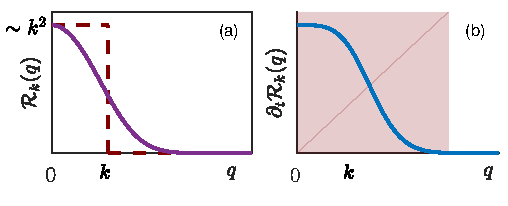
\includegraphics[width=0.95\columnwidth]{RegDerReg.pdf}
\end{center}
\vspace*{-22pt}
\caption{(a) Allure du régulateur, choisi pour une valeur de $k$ donnée, ayant une décroissance exponentielle entre $\simeq k^2$ et $0$. Quand le régulateur à cette allure nous avons approximativement intégrés les degrés de libertés correspondant à des moments de norme dans $\simeq [k,\Lambda]$ uniquement. (b) Allure de la dérivée temporelle du régulateur choisi pour une valeur de $k$ donnée (ligne continue bleue).}
\label{fig:RegDerReg}
\end{figure}
Introduisons maintenant la différence principale du NPRG avec le RG : un calcul par le potentiel de Gibbs.


\subsubsection{Différence avec le RG : potentiel de Gibbs}

Ce n'est pas vraiment $\Zc_k$ que nous calculons directement dans le calcul du NPRG mais une grandeur qui s'exprime en fonction de $\Zc_k$ : \textit{le potentiel de Gibbs effectif}. On le note $\Gamma_k$. Pour tout $k$, notons que $\Zc_k$ peut se calculer en connaissant $\Gamma_k$. On peut notamment obtenir $\Zc = \Zc_{k\to 0}$ en connaissant le \textit{potentiel de Gibbs} $\Gamma = \Gamma_{k \to 0}$. Définissons donc cette grandeur. On se place à $k$ fixé.  On peut définir le potentiel de Gibbs effectif par
\begin{equation}
  \Gamma_k [\phiv] = - \ln(Z_k[\bv]) + \int_{\Omega} \bv \phiv \, \dd \,\rv- \Delta H_k[\phiv]\, ,
\end{equation}
avec $\phiv$, la moyenne statistique du champ, définie comme 
\begin{equation}
  \phiv[\pv, \bv]  \equiv \left< \varphiv(\pv) \right> \equiv \frac{1}{\Zc[\bv]} \int \Dc \varphiv \exp \( - \Hc[\varphiv, \bv] \) \varphiv \, .
\end{equation}
Dans le langage du modèle d'Ising 2D, $\phiv$ correspond à l'aimantation $m$. On donne aussi une notation pour les dérivées fonctionnelles de $\Gamma_k$ en TF avec 
\begin{equation}
\Gamma^{(n)}_{k, \{i_j\}}[\{\pv_j\}; \phiv] = \derd{^n \Gamma_k [\phiv]}{\phiv_{i_1}(-\pv_1)...\delta \phiv_{i_2}(-\pv_n)} \, ,
\end{equation}
et on note plus spécifiquement
\begin{equation}
\Gamma^{(2)}_{k,ij}[\pv; \phiv]  \equiv \Gamma^{(2)}_{k,ij}[\pv, - \pv; \phiv] = \derd{^2 \, \Gamma_k [\phiv]}{\phiv_{i}(-\pv)\delta \phiv_{j}(\pv)} \, .
\end{equation}
\indent
En utilisant $\Zc_k$ nous pouvons aussi définir des fonctions de corrélations comme nous l'avons fait pour le modèle d'Ising 2D et qui sont à la base de la définition des coefficients $\eta$ et $\nu$. Il est possible de se reporter à \refann{Prop} pour plus de détails. Nous considérons simplement ici qu'il est possible de définir $G_{k}$ que l'on nomme le propagateur, égal à une fonction de corrélations à deux points. Cette fonction est liée au potentiel de Gibbs par la relation (au sens de l'inverse d'opérateur, c.f \refann{FuncCorrel}),
\begin{equation}
  G_{k}[\pv ; \phiv] = \(\Gamma^{(2)}_{k}[\pv, \phiv] + \Rc_k(\pv)\)^{-1} 
  \label{eq:propG}
\end{equation}


\commentout{
On peut donc, à partir de ces définitions, obtenir une équation différentielle sur $\Gamma_k$ pour lequel on connait une condition initiale. Avec cette équation il est possible de calculer $\Gamma = \Gamma_{k \to 0}$ et donc aussi $\Zc$. \\}



\subsubsection{Équation fondamentale : équation de flot}

On peut utiliser les définitions que l'on vient de poser pour présenter l'équation fondamentale du NPRG que l'on appelle l'équation de flot exacte de $\Gamma_k$. Il s'agit d'une équation valable pour $k \in ]0, \Lambda]$ décrivant l'évolution de $\Gamma_k$ avec $k$ lorsqu'on le fait évoluer de $\Lambda$ à $0$. On définit une nouvelle variable $t$ appelée temps du RG.
\begin{equation}
	t = \ln(k/\Lambda), \quad \text{donnant} \quad \partial_t \, ... = k\partial_k \, ...
\end{equation}
Quand $k$ varie de $\Lambda$ vers $0$, $t$ varie de $0$ vers $-\infty$, c'est donc un "temps" négatif. On montre alors \cite{Delamotte2012},

\begin{equation}
\partial_t \Gamma_{k}	[\phiv] = \frac{1}{2} \sum\limits_{i=1}^{N} \sum_\qv \partial_t \Rc_k(\qv) \, G_{k, ii}[\qv; \phiv] \, ,
	\label{eq:flot}
\end{equation}
\begin{equation}
	\Gamma_\Lambda [\phiv] = H[\phiv] \, .
	\label{eq:initFlotBMW}
\end{equation}
Nous avons une équation différentielle avec une condition initiale $\Gamma_\Lambda$ connue permettant d'accéder à $\Gamma_{k \to 0} = \Gamma$. Notons que l'on mélange dans cette équation les notations équivalentes $t$ et $k$ par convention. \\



Un problème subsiste tout de même : pour pouvoir réaliser un calcul numérique il faut, dans cette équation, faire un calcul à $\phiv$ uniforme.
On introduit le potentiel $V_k$ effectif en $\phiv$ uniforme par
\begin{equation}
V_k(\phiv) \equiv \frac{1}{|\Omega|} \Gamma_k[\phiv]|_{\phiv \text{ unif.}}.
\end{equation}
Rappelons que l'on note avec une parenthèse les fonction de $\phiv$ vecteur dans $\R^N$ et entre crochet les fonctionnelles dépendant des fonctions $\phiv \in \(C^0(\Omega)\)^N$. Ainsi numériquement nous pouvons seulement essayer de résoudre l'équation de flot (exprimée ici après être passé dans la limite thermodynamique $|\Omega| \to \infty$),
\begin{equation}
	\partial_t V_k(\phiv) = \frac{1}{2} \sum\limits_{i=1}^{N} \int_\qv \partial_t \Rc_k(\qv) \, G_{k, ii}(\qv; \phiv) \, ,
\end{equation}
Le potentiel du système $V = V_{k \to 0}$ que nous pourrions alors calculer nous suffit pour connaitre le comportement macroscopique du système. Cependant si l'on veut connaitre $\partial_t V_k(\phiv)$ il nous faut connaitre $G_k(\pv, \phi)$ qui s'exprime en fonction de $\Gamma_k^{(2)}(\qv, \phiv)$. Il s'avère que $\Gamma_k^{(2)} (\qv, \phiv)$ peut se calculer connaissant la fonctionnelle $\Gamma_k[\phiv]$ mais pas la fonction $V_k(\phiv)$. La seule façon de connaitre $\Gamma_k^{(2)}(\qv, \phiv)$ serait de résoudre l'équation de flot exacte de $\Gamma_k^{(2)}(\pv, \phiv)$ (que l'on peut déduire de celle de $\Gamma_k[\phiv]$). Le problème se répète alors car cette nouvelle équation fait intervenir des dérivées supérieures de $\Gamma_k$ que nous ne pouvons pas connaitre non plus. On dit que l'équation est ouverte : elle n'est pas soluble. L'approximation BMW permet de résoudre ce problème. 


\vspace*{11pt}



\subsection{Approximation BMW de l'équation fondamentale du NPRG (pour $\mathbb{Z}_2$)} 
 
Pour rester concis, nous nous intéressons dans cette section au cas particulier de la symétrie $\mathbb{Z}_2$ (correspondant à $O(N)$ pour $N=1$)\footnote{i.e. lorsque l'hamiltonien $H$ satisfait $H[-\varphiv] = H[\varphiv]$. Le cas général des équations pour $N$ quelconque se trouve dans \cite{benitez2012nonperturbative}.}. Nous présentons l' équation dite de "flot BMW" qui est issue de l'approximation BMW appliquée à l'équation de flot du NPRG\footnote{La méthode pour trouver ces équations n'est pas expliquée ici mais on la trouvera dans \cite{Blaizot}.}. Il s'agit plus précisément d'une équation portant sur
\begin{equation}
	\Gamma_{k}^{(2)}(\pv, \phi) \equiv \Gamma_{k}^{(2)}[\pv, \phi] {|}_{\phi \text{ unif.}} \,
\end{equation}
qui est lié à la fonction de corrélation à deux points $G_k$ (c.f. \refeq{propG}). La fonction $\Gamma^{(2)}(\pv, \phi) = \Gamma_{k\to 0}^{(2)}(\pv, \phi)$ permet donc aussi de calculer les exposants critiques $\eta$ et $\nu$.
On montre (dans la limite thermodynamique),
\begin{equation}
\begin{split}
	\partial_t \Gamma_{k}^{(2)}(\pv, \phi) = & \quad J_3(\pv, \phi) {\( \partial_\phi \Gamma_{k}^{(2)}(\pv, \phi) \)}^2 \\
	& - \frac{1}{2}  I_2(\phi) \, \partial_\phi^{2} \Gamma_{k}^{(2)}(\pv, \phi) \, ,
\end{split}
\label{eq:flotBMW}
\end{equation}
où l'on a introduit par concision,
\begin{equation}
\begin{split}
	J_n(\pv,\phi) & = \int_\qv \partial_t \Rc_k(\qv) \,G_k(\pv+\qv, \phi) \,G_k^{n-1}(\qv, \phi) \, ,  \\
	I_n(\phi) & = J_n(\pv = 0, \phi) = \int_\qv \partial_t \Rc_k(\qv) \,G_k^{n}(\qv, \phi) \, .
\end{split}
\label{eq:JI}
\end{equation}
Notons que les intégrales dans cette équation de flot sont tronquées par la fonction $\qv \to \partial_t \Rc_k(q)$ qui, par les propriétés imposées de $\Rc_k$, est une fonction décroissante fortement vers $0$ pour tout $k$ quand $\|\qv\|_2 \to \infty$ (c.f. \refig{RegDerReg} (b)). Ceci est important pour la résolution numérique. \\

Cette équation est soluble numériquement. Sa condition initiale vient de \refeq{initFlotBMW},  
\begin{equation}
	\Gamma^{(2)}_\Lambda(\pv, \phi) = \left. \derd{^{(2)}H[\phi]}{\phi(-\pv)\delta\phi(\pv)} \right|_{\phi \text{ unif.}}
	\label{eq:initBMW}
\end{equation}
Nous n'avons cependant pas de conditions aux bord pour l'équation de flot BMW en $\pv$ et $\phi$. Ceci ne pose pas de problème et pourra tout de même être traité numériquement. On fait l'hypothèse physique qu'il existe une solution et une seule à ces équations. Enfin, pour conserver une précision maximale dans l'approximation cette équation pourra être couplée à l'équation de flot du potentiel effectif $V_k$ qui fait intervenir $\Gamma_k^{(2)}(\pv, \phi)$ que nous pouvons maintenant calculer.



\vspace*{11pt}
\subsection{Détermination de la température critique : notion de point fixe}

Le premier objectif de notre étude est de trouver la valeur des exposants critiques des systèmes que l'on étudie. Ces exposants sont définis par la fonctions de corrélation à deux points, qui est liée à $\Gamma^{(2)}$, mais ils ne sont définis qu'à la température critique que l'on ne connait pas a priori sur un système donné. Comme dans nos notations on inclus le terme $k_BT$ dans l'expression de l'hamiltonien $H$, la température à laquelle est soumise le système est contenue dans $H$ et la condition initiale de nos équations de flots dépend de $H$. Il faut donc trouver la température dans l'expression de $H$ qui correspond à $T_c$ pour avoir une chance de calculer $\eta$ et $\nu$. Le second objectif de notre étude se concentre même sur le calcul de $T_c$ pour un système particulier. 

Une question se pose alors : comment sait-on si la température introduite est la température critique ? La température à laquelle est soumise le système est la température critique si l'on obtient une solution de \textit{point fixe} à notre équations de flot BMW. \\

Sans entrer dans le détail, pour trouver une telle solution on réécrit l'équation de flot BMW en \textit{l'adimensionnant}. C'est à dire que l'on divise par certaines longueurs caractéristiques toutes les variables et fonctions de l'équation pour obtenir de nouvelles variables et fonctions qui n'aient plus de dimension de longueur. Il en résulte une nouvelle équation : l'équation de flot BMW \textit{adimensionnée}. On note par exemple $\tilde{\Gamma}_k^{(2)}$ la fonction dite adimensionnée de $\Gamma_k^{(2)}$ : elle est sans dimension de longueur, dépend de variable sans dimension de longueur et est solution de l'équation adimensionnée. \\
\indent
Trouver une solution de point fixe se traduit, dans notre cas, par trouver une solution de l'équation de flot BMW adimensionnée $\tilde{\Gamma}^{*(2)}_k$ telle que
\begin{equation}
\lim\limits_{k \to 0} \partial_t \tilde{\Gamma}^{*(2)}_k = 0,
\label{eq:ptFixe}
\end{equation}
Pour trouver la température critique d'un système on cherche donc une solution ayant cette propriété en faisant varier la température dans la condition initiale\footnote{Cette recherche ne se fait pas aléatoirement et peut être réalisée à l'aide d'une dichotomie.}. C'est donc plus exactement $\Gamma^{*(2)} = \tilde{\Gamma}^{*(2)}_{k \to 0}$, correspondant à un système soumis à sa température critique, qui nous permet de donner une valeur à $\eta$ et $\nu$. \\






\subsection{Résumé de la méthode}

En résumé, nous recherchons à calculer les exposants critiques et la température critique de différents systèmes. Pour cela nous utilisons le NPRG couplé à l'approximation BMW qui nous permet d'obtenir une équation différentielle, sur une grandeur notée $\Gamma^{(2)}_k$, dont on connait une condition initiale en $k = \Lambda$ et que l'on peut résoudre numériquement pour obtenir $\Gamma^{(2)} = \Gamma^{(2)}_{k \to 0}$. Cette grandeur est importante car elle est reliée à une fonction de corrélations à deux points qui définit les exposants critiques.

Les exposants critiques d'un système ne sont définis que lorsqu'il est soumis à sa température critique. Il nous faut donc la déterminer. Pour trouver la température critique du système il est faut \textit{d'adimensionner} l'équation BMW et en rechercher une solution dite de \textit{point fixe} que l'on sait caractériser par son comportement en $k \to 0$. La température à laquelle est soumise un système se trouve dans la condition initiale des équations BMW et la solution de l'équation BMW est la solution de point fixe noté $\tilde{\Gamma}^{* (2)}_k$ si et seulement si la température dans la condition initiale correspond à la température critique. Trouver une solution de point fixe nous assure donc d'avoir inscrit $T=T_c$ dans la condition initiale. Ainsi on détermine $T_c$.

On peut alors définir une grandeur associée $\eta_k^*$ à $\tilde{\Gamma}^{* (2)}_k$ et $\eta$ est obtenu, par exemple, en prenant $\eta = \lim_{k\to 0} \eta_k^*$. Détaillons dans la section suivante cette procédure en pratique dans le cas de la résolution de ces équations pour ce que l'on nomme le modèle continu. 

\newpage


 
\section{Le modèle continu $O(N)$}

\label{sec:Continu}

Abordons maintenant la première étude que nous avons réalisé, portant sur la recherche des exposants critiques des systèmes possédant une symétrie $O(N)$.


\subsection[Modèle continu]{Hamiltonien de la théorie $\varphiv^4$ : \\ modèle continu}

Il a été montré \cite{Bellac2012} que lorsque l'on cherche à déterminer les exposants critiques, et que l'on s'intéresse uniquement à ce qu'il peut se passer au voisinage de la température critique alors il suffit d'étudier les premiers ordres du hamiltonien du système isolé autour de $\varphiv \sim 0$, qui, pour respecter les symétries, dans le modèle $O(N)$ a nécessairement la forme 
\begin{equation}
		H[\varphiv] = \int_\rv \, \left\{ \frac{1}{2}(\nabla \varphiv)^2 + \frac{1}{2}r_0 \varphiv^2 + \frac{u_0}{4!}{\({\varphiv}^{2}\)}^{2} \right\}
		\label{eq:hamiltCont}
\end{equation}


Avec $u_0$ et $r_0$ deux réels. On retrouve l'hamiltonien $\varphiv^4$ déjà mentionné dans l'introduction. Comprenons que cet hamiltonien n'est pas le vrai hamiltonien de tous les systèmes régit pas une symétrie $O(N)$ mais il suffit à en déduire les grandeurs universelles aux transition de phase. En effet il s'agit d'un modèle simplifié avec les même symétries que les systèmes qui nous intéresse. Or rappelons que les grandeurs universelles comme les exposants critiques sont justement dites universelles car elles sont identiques pour deux systèmes ayant les mêmes propriétés de symétrie. \\
\indent
La température à laquelle est soumise ce système se trouve définie\footnote{Notons que l'hamiltonien ne dépend normalement pas de la température. Il se trouve que c'est ici le cas car on a introduit $k_BT$ dans l'expression de $H$ et nous avons renormalisé le champ pour que le terme devant le gradient soit $1/2$.} dans le paramètre $r_0$. Notons que comme la température critique $T_c$ n'est pas une donnée universelle celle du modèle représenté par cet hamiltonien n'est pas commune à tous les systèmes ayant une symétrie $O(N)$ mais elle est plus facile à déterminer numériquement. \\

Introduisons maintenant les équations BMW que nous avons tenté de résoudre, pour le hamiltonien que nous venons de présenter
\\



\subsection{Système d'équations BMW continu}


On se concentre par simplicité sur le cas  $\mathbb{Z}_2$ uniquement. On utilise à partir de maintenant la variable\footnote{Cette variable n'est pas vraiment différente de $\phi$ dans le cas $\mathbb{Z}_2$ mais elle l'est dans le cas $O(N)$ en général ou $\phiv$ est un vecteur.} scalaire $\rho = \phi^2/2$. Grâce à l'invariance par rotation dans $\R^d$ de $H$ en fonction de $\pv$, les différentes grandeurs que la considère ne dépendent plus entièrement des moments $\pv$ (ou $\qv$, ou $\pv+\qv$) mais seulement de $\pv^2$ (ou $\qv^2$, ou $(\pv+\qv)^2$ et donc de la norme $p = \| \pv \|_{2}$ (ou q, ou $\|\pv+\qv\|_2$). \\

L'équation de flot BMW (cf. \refann{BMWON}), couplée à l'équation du potentiel effectif du système, se réécrit, une fois \textit{adimensionnée}, donne le problème à résoudre : \\

\noindent
{\itshape Trouver $\tY_k(\tp, \trho)$ et $\tW_k(\trho)$ tels que pour tout $k \in ]0 ,\Lambda]$,  $\trho \in [0, +\infty[$ et $\tp \in [0, +\infty[$,}
\begin{align*}
	\partial_t  \tY_k(\tp, \trho) & = 
	\begin{aligned}[t]
			& \eta_k(1+\tY_k(\tp, \trho)) + \tp \, \partial_{\tp} \tY_k(\tp, \trho) \\
			 &  -(2-d-\eta_k)\trho \,\partial_{\trho} \tY_k(\tp, \trho)  \quad  \\
			& + 2\trho \tp^{-2} \left[ {\( \tp^2 \partial_{\trho} \tY_k(\tp, \trho) + \tilde{u}_k(\trho)\)}^2\, \tJ_3(\tp, \trho) \right] \\
			 & - 2\trho \tp^{-2} \left[ \tilde{u}_k^2(\trho)  \tI_3(\trho) \right] \\
			&  - \tI_2(\trho) \(  \partial_{\trho} \tY_k(\tp, \trho) / 2 + \trho \,  \partial_{\trho}^2 \tY_k(\tp, \trho) \)
	\end{aligned}
	\label{eqn}\\
	\partial_t  \tW_k &  = 
	\begin{aligned}[t]
		& (\eta_k-2) \tW_k(\trho) \\
		& + (d-2+\eta_k) \trho \,\partial_{\trho}\tW_k(\trho) + \frac{1}{2} \partial_{\trho} \tI_1(\trho) \, ,
	\end{aligned}
\end{align*}
\textit{avec la définition}
\begin{equation}
\begin{split}
\eta_k = \frac{1}{2}  \tI_2(\trho = 0)\partial_\rho\tY_k(\tp = 0, \trho = 0) \,, 
\end{split}
\end{equation}
\textit{et les conditions initiales,}
\begin{equation}
	\tY_\Lambda(\tp, \trho) = 0 \quad  \text{et} \quad \tW_\Lambda(\trho) = \tilde{r}_0 + \tilde{u}_0\trho
\end{equation}
où $\tilde{r}_0$ et $\tilde{u}_0$ viennent de $r_0$ et $u_0$ (c.f. \refeq{hamiltCont}). Les intégrales $\tI_n$ et $\tJ_n$ sont de la même forme que $I_n$ et $J_n$ introduites en \refeq{JI} : $\tJ_n(\tp, \trho) \propto J_n(\pv, \rho)$ et donc $\tI_n \propto I_n$ aussi. La fonction $\tilde{u}_k$ est définie en \refann{BMWON}. On rappelle que $t = \ln(k/\Lambda)$ et $\partial_t ... = k \partial_k ...$. Nous faisons l'hypothèse physique selon laquelle il existe une solution et une seule à ce problème.\\

Pour chercher la température critique du système on cherche une solution de point fixe. C'est à dire que l'on résout le système différentiel précédent pour différentes valeurs de $\tilde{r}_0$. Pour cela on teste plusieurs $\tilde{r}_0$ avec une dichotomie et avec des valeurs initiales prises aléatoirement jusqu'à ce que l'on trouve la solution $(\tY_k^*, \tW_k^*)$ telle que $\lim_{k\to 0} \partial_t \tW_k^* = 0$ et $\lim_{k\to 0} \partial_t \tY_k^* = 0$. Cette condition correspond, avec la définition de $\tY$ et $\tW$, à la définition d'un solution de point fixe $\tilde{\Gamma}_k^{*(2)}$ (c.f. \refeq{ptFixe}). \\

On peut aussi montrer qu'avec la définition donnée de $\eta_k$, si l'on à l'on a introduit la température critique comme température dans la condition initiale alors on retrouve l'exposant critique $\eta$ avec
\begin{equation}
	\lim_{k \to 0} \eta_k = \eta	
\end{equation}




\subsection{Régulateur pour BMW continu}

Dans l'expression des intégrales $\tI_n$ et $\tJ_n$ apparait la fonction que l'on appelle le régulateur du NPRG. Pour satisfaire à toutes les conditions d'un régulateur on utilise une expression (c.f. \refig{RegDerReg} (a)) infiniment dérivable à décroissance exponentielle définie par (et implicitement prolongée par continuité en $q = 0$)
\begin{equation}
	\forall q \in [0, \Lambda] \quad \Rc_k(q) = \alpha \frac{q^2}{\exp{(q^2/k^2)}-1}
	\label{eq:RegExp}
\end{equation}
Avec $\alpha$ un réel positif que l'on prend de l'ordre de l'unité et que l'on peut faire varier mais qui n'est pas supposé changer les résultats des calculs. Le caractère régulier (au sens infiniment dérivable) de ce régulateur est nécessaire pour assurer des résolutions numériques stables dans les équations BMW.  

\commentout{
Remarquons que l'on satisfait bien aux conditions aux limites imposées sur le régulateur car 
\begin{equation}
	\forall k \in ]0,\Lambda],  \quad \underset{q \in [0, \Lambda]}{ \text{Sup}} \left\{ \Rc_k(q) \right\} = \alpha k^2
\end{equation}
donc $\Rc_k$ converge même uniformément vers 0 quand $k$ tend vers 0, (C1) définie en \refsec{Reg} est vérifiée. En outre, (C2) est aussi validée puisque
\begin{equation}
	\underset{q \in [0, \Lambda]}{ \text{Inf}} \left\{ \Rc_\Lambda(q) \right\} = \alpha \frac{\Lambda^2}{e-1}
\end{equation}
}

\vspace*{11pt}

\section{Méthodes numériques pour la résolution de BMW continu}

\label{sec:NumContinu}

\subsection{Travail réalisé}


La première partie de notre travail a été de reprendre le développement de ces équations et nous avons réécrit de façon plus modulable et structurée en C++ un code de résolution qui avait déjà été écrit au laboratoire (c.f. \refig{org}). Pour résoudre ces équations de très nombreuses méthodes numériques avaient déjà été mises en place, comme des méthodes Galerkin \cite{shen1994efficient, LeonardThesis} pour la représentation des fonctions, de Simpsons pour le calcul des intégrales, de Runge-Kutta pour la discrétisation temporelle etc., avant qu'un algorithme fonctionnant dans les cas $N=1$ et $d=2$ puisse être trouvé. Cependant, cet algorithme échoue lorsque l'on essaie de l'utiliser en $N \ge 2$ et $d=2$. Nous avons donc essayé d'en comprendre la cause en modifiant certains paramètres et certaines implémentations des algorithmes pour différentes valeurs de $N$ et de $d$. Nous avons aussi réalisé des calculs en les comparant à d'autres codes plus simples (que nous avons réécrits ou qui avaient déjà été écrits auparavant), provenant d'autres approximations que BMW. 


\subsection{Structure de l'algorithme}

Nous avons à résoudre ici un système d'équations intégro-différentielles non linéaires couplées et sans conditions au bords. Pour cela nous utilisons différentes techniques numériques. \\

Pour la discrétisation en "temps" $t$, nous sommes dans l'obligation d'utiliser un schéma explicite à cause de la structure complexe des termes de gauche des équations. Il a été mis en évidence dans ce code qu'un schéma d'Euler explicite d'un pas de temps est suffisant pour obtenir une résolution stable, c'est donc ce qui est utilisé. \\

Ensuite nous différencions la dépendance en champ (i.e. en $\trho$) à celle en moment (i.e. $\tp$) des fonctions inconnues. Pour ce qui est de la dépendance en champ, il suffit de prendre une grille fixe finie de points $\{ \trho_i \}_i$ régulièrement espacés dans $[0, \trho_{max}]$, où $\trho_{max}$ est choisi suffisamment grand. Les dérivées selon cette variable se calculent alors par des schémas différences finis d'ordre 5. \\

Enfin pour la dépendance en moment la discrétisation se fait dans une boite $[0, \tp_{max}]$ où $\tp_{max}$ est choisi aussi suffisamment grand. Cependant les choses sont plus compliquées car il faut à la fois pouvoir facilement calculer des dérivées selon $\tp$, mais aussi intégrer selon cette même variable afin d'obtenir les intégrales $\tI$ et $\tJ$.  Le calcul des intégrales $\tJ(\tp, \trho)$ pour tout $\tp$ et $\trho$ de la discrétisation est ce qui demande le plus de temps dans l'exécution du code. Dans ces premières versions la discrétisation était faite sur une grille fixe de points régulièrement espacés et les intégrales étaient calculées par des méthodes de Simpson. Cependant cela s'est avéré ne pas être assez précis dans certaines configurations, les algorithmes n'étaient pas robustes. Pour palier à ce problème et pour calculer correctement $\tilde J_3$ c'est une décomposition pseudo spectrale de la partie en moment des fonctions inconnues qui a été mise en place dans la version sur laquelle nous avons commencé à travailler. Plus précisément, la dépendance en moment des fonctions inconnues est exprimée par une décomposition en série de polynômes de Tchebytchev. 

La décomposition pseudo-spectrale signifie alors qu'à chaque pas de temps $t=\ln(k/\Lambda)$ de la résolution on calcule et conserve en mémoire pour le pas de temps suivant la valeur de la fonction au point d'interpolation ainsi que les coefficients de sa décomposition en série de polynôme de Tchebytchev. Les intégrales peuvent alors être calculées par une quadrature de Gauss-Legendre. \\

Nous détaillons alors les différents aspects numériques des discrétisations que nous avons utilisé.




\subsection{Discrétisation en champ}

Comme nous l'avons mentionné, la discrétisation en champ se fait sur une grille fixe de points régulièrement espacés. Les dérivées sont calculées sur 5 points avec des schémas aux différences finies (\refann{Der5}). Ce choix sur 5 points  a été fait pour essayer de calculer des dérivées le plus précisément possible. Le problème vient alors des points des bords de la grille de discrétisation, puisque nous ne possédons pas de condition de bords à nos équations. Ainsi, nous utilisons des schémas complètements décentrés pour ne faire un calcul que sur les points connus dans la grille. Il s'avère que cette technique reste stable (nous détaillons en \refsec{Problemes} que cela nous a quand même posé des problèmes pour le modèle d'Ising en deux dimensions). \\

Nous avons remarqué aussi que l'on retrouve l'équivalent d'une condition de Courant-Friedrichs-Lewy (CFL) \cite{courant1967partial} pour le choix du pas de discrétisation $\delta \rho$. En effet le rapport $\delta t / \delta\rho$ doit rester inférieur à une certaine valeur pour conserver la stabilité du schéma.\\

Enfin il pourrait sembler étrange d'utiliser une discrétisation en champ d'ordre 5 couplée à une discrétisation en temps $t$ d'ordre 1. Cependant l'implémentation d'un schéma de Runge-Kutta a été testée sans pour autant permettre un calcul plus précis ou plus rapide. 


%\vspace*{11pt}


\subsection{Calcul des intégrales}

Le plus gros problème rencontré dans la formulation discrétisée du problème a été le calcul des intégrales $\tJ$. 
Grâce aux symétries des fonctions que l'on intègre on peut développer une expression de ces intégrales telle que la dimension $d$ devienne un simple paramètre. En effet calculer l'intégrale $\tJ_n$ revient à calculer 
\begin{equation}
\tJ_n(\tpv,\trho) = \int_{\R^d} f(\tqv^2,\trho)g((\tpv+\tqv)^2,\trho) \, \dd \, \tqv \, ,
\end{equation}
où $f$ et $g$ sont deux fonctions. Et il en est de même pour les intégrales $\tI$ en prenant $\tpv = 0$ dans l'expression précédente. On pose alors $\tqv = \tq_1 \uv + \tqv_2$, où $\uv = \tpv/\|\tpv\|$ et $\tqv_2$ est orthogonal à $\uv$. Il vient alors, avec $\tp = \|\tpv\|^2$,
\begin{equation}
\tJ_n(\tp, \trho) = S_{d-1} \int_0^{+\infty} \dd\tq_2 \, \tq_2^{d-2} \int_{-\infty}^{+\infty} \dd\tq_1 \, h (\tp, \tq_1, \tq_2, \rho) \, ,
\end{equation}
en posant
\begin{equation}
h (\tp, \tq_1, \tq_2, \trho) \equiv f(\tq_1^2 + \tq_2^2, \trho) g(\tp^2 + \tq_1^2 + \tq_2^2 + 2\tp\tq_1, \trho) \, .
\end{equation}
Le coefficient $S_{d-1}$ est un pré-facteur réel. De ce fait, le calcul d'une intégrale à $d$ dimensions se ramène au calcul de deux intégrales seulement, qui peut être fait chacun sans problèmes avec une interpolation de Gauss-Legendre (\refann{Quad}). En pratique, les intégrales étant coupées par le régulateur nous réalisons l'intégration jusqu'à une borne $\tq_{max}$ telle que $\|\tqv\|_2 < \tq_{max} < \tp_{max}$ (où $\tp_{max}$ est la borne supérieure de la discrétisation en moments). Comme on fait l'hypothèse vraisemblable selon laquelle les inconnues de notre système à résoudre son régulières on peut réaliser l'intégration efficacement en utilisant un quadrature de Gauss-Legendre. En notant, $\{\xi_i\}_{i \in \bbrac{1, n_{gl}}}$ les points de la quadrature de Gauss-Legendre et $\{w_i\}_i$ les poids associées nous calculons 
\begin{equation}
\begin{split}
\tJ_n(\tp, \trho) \simeq S_{d-1}\frac{\tq_{max}^2}{2} \sum_{i = 1}^{n_{gl}} w_i \left[ \frac{\tq_{max}}{2\sqrt{2}}\( 1+ \xi_i \) \right]^{d-2} \\
\times \sum_{j=1}^{n_{gl}} w_j h\(\tp,\frac{\tq_{max}}{2\sqrt{2}}\( 1+ \xi_i \), \frac{\tq_{max}}{\sqrt{2}} \xi_j , \trho\)
\end{split}
\end{equation}


%\vspace*{11pt}

\subsection{Discrétisation en moment}



\subsubsection{Expression des coefficients}

\label{sec:ExprCoeff}

Pour la discrétisation en moments, afin de pouvoir calculer, entre autre, les intégrales précédentes, nous avons choisi d'utiliser des polynômes de Tchebytchev. Dans \cite{Tchebychev} il est démontré les propriétés suivantes : \\

\noindent 
\textbf{Décomposition sur une base de Tchebytchev}. {\itshape 
Soient $a$, $b$, deux réels tels que $b>a$. Soit f une fonction de classe $\Cc^{0}$ de $[a,b]$ dans $\R$.
On note $T_j$ est le polynôme d'ordre $j$ de Tchebytchev de première espèce. Soit $n \in N$ et $\{x_k\}_{k\in\bbrac{0, n}}$ les racines du polynôme $T_{n}$, on pose
\begin{equation}
c_j = \frac{A_j}{n} \sum\limits_{k = 0}^{n-1}f\(\frac{a+b}{2} + x_k \frac{b-a}{2}\) T_j(x_k) 
\end{equation}
\begin{equation}
S_n[f](x) = \sum\limits_{j = 0}^{n - 1} c_j T_j\(\frac{2x-a-b}{b-a}\) \quad \forall x \in [a,b]
\end{equation}
Avec $A_j = 2$ si $j > 0$ et $A_0 = 1$. \\
\noindent
Nous avons alors, en norme $L^2$,
\begin{equation}
\lim\limits_{n\to \infty} \|f - S_n[f] \|_2 = 0
\end{equation}
De plus si $f$ est $\Cc^{1}$ alors
\begin{equation}
\lim\limits_{n \to \infty}  \|f - S_n[f] \|_\infty = 0
\end{equation}
On écrit, pour $n$ suffisamment grand, $f \simeq S_n[f]$. \\
}

\commentout{
\le \frac{(b-a)^{n}}{2^{2n-1} n!}\underset{x \in [a,b]}{\mathrm{Sup}} |f^{(n+1)}(x)

\begin{equation}
	c_j = \left< T_j, f \right>_T^{a,b}\equiv \frac{2}{b-a}\int_{a}^b{ \frac{f(y) T_j(\frac{2y-a-b}{b-a})}{\sqrt{1-{\( \frac{2y-a-b}{b-a} \)}^2}} \dd \, y}
\end{equation}

\underset{x \in [a,b]}{\mathrm{Sup}}
}


La présence du régulateur à été introduite dans le NPRG pour permettre de gagner en régularité dans les équations et pouvoir effectuer des calculs de manière continue (contrairement au RG, où l'on procède par itérations successives). Avec le régulateur $\Cc^\infty$ que nous avons choisi, on peut supposer que la solution $(\tY, \tW)$ du système est un couple de fonctions extrêmement régulières. Nous pouvons au moins, pour appuyer ce propos, étudier la régularité des fonctions du schéma semi-discrétisé en temps. \\
\indent
On pose $n \in \N$. On note $(t_0, t_1, .. t_n, ..)$ l'ensemble des temps discrets utilisés dans le schéma d'Euler. On note $\tY_{k_n}$ la fonction $\tY_k$ au temps discret $t_n$. Nous avons montré que, sous certaines hypothèses cohérentes avec ce que l'on souhaite obtenir, la fonction $\tY_{k_n}$ est une fonction régulière (au moins de classe $\Cc^1$) sur $[0, +\infty[^2$ et donc sur $[0, \tp_{max}]$. Ceci justifie alors l'utilisation des polynômes de Tchebytchev pour l'interpolation des fonctions dépendant d'un moment. On utilise donc les propriétés précédentes pour $a=0$ et $b = \tp_{max}$. 

 %\vspace*{11pt}



\subsubsection{Méthode de Clenshaw}


Afin de calculer la fonction aux points d'interpolation lorsque cela est nécessaire nous utilisons une méthode un peu plus astucieuse que celle consistant à calculer directement la somme de la série. \\

\noindent
\textbf{Algorithme de Clenshaw}. {\itshape
Soit, une suite de polynômes $\{\Pc_m\}_{m \in \N}$ liés par la relation, pour tout $x \in [-1,1]$, 
\begin{equation}
 \Pc_{m+1}(x) = u_m(x)\Pc_m(x) + v_m(x)\Pc_{m-1}(x)
\end{equation}
On souhaite calculer, pour $x \in [-1, 1]$ et $\{a_l\}_l$ donnés, 
\begin{equation}
  S = \sum_{l=0}^{n} a_l \Pc_l(x)
\end{equation}
On considère l'algorithme suivant :
\vspace*{-11pt}
\begin{algorithm}[H]
  \begin{algorithmic}[1]
    \STATE $b_{n+2} = 0$ ; $b_{n+1} = 0$
    \FOR{ $m = n .. 1$  }
    \STATE $b_m = a_m + u_m(x)b_{m+1} + v_{m+1}(x)b_{m+2}$
    \ENDFOR
    \STATE $S_1 = a_0\Pc_0(x) + b_1\Pc_1(x) + b_2v_1(x)\Pc_0(x)$
  \end{algorithmic}
\end{algorithm}
\vspace*{-11pt}
\noindent
Alors nous avons\footnote{Ce résultat se démontre par récurrence sur $m \in \bbrac{1,N}$ en remarquant que,
$S_1 = S_m +  b_{m+1}\Pc_{m+1}(x) + b_{m+2}v_{m+1}(x)\Pc_{m+2}(x)$\\
Avec la notation $S_m = \sum_{l=0}^{m} a_l \Pc_l(x)$.} $S = S_1$. 
} \\

Ainsi, pour calculer $f(x)$ pour $x \in [a,b]$, pour une décomposition en série de polynômes de Tchebytchev nous obtenons l'algorithme

\begin{algorithm}[H]
  \begin{algorithmic}[1]
    \STATE $b_{n+2} = 0$ ; $b_{n+1} = 0$
    \STATE $y = (2x-a-b)/(b-a)$
    \FOR{ $m = n .. 1$  }
    \STATE $b_m = a_m + 2yb_{m+1} - b_{m+2}$
    \ENDFOR
    \STATE $f(x) = a_0 - b_2 + b_1y$
  \end{algorithmic}
\end{algorithm}

Cette méthode \cite{clenshaw1955note} est plus robuste et légèrement plus rapide que celle qui consisterait à calculer directement la somme de la série de polynômes. En effet, on passe d'un algorithme avec $\sim 4n$ opérations à une algorithme avec $\sim 3n$ opérations en utilisant cette technique pour des polynômes de Tchebytchev. Le gain est faible mais cela sera peut être utile en dimension 2 pour le modèle d'Ising 2D (c.f. \refsec{NumIsing}). \\


\subsubsection{Calcul des dérivées}

Un autre avantage d'exprimer les fonctions sous une décomposition en série de polynôme de Tchebytchev pour la variable de moment $\tp$ est qu'il devient facile d'en calculer les dérivées par rapport à $p$ en tout point de la boite $[0, \tp_{max}]$ de discrétisation. En effet il existe une relation simple entre les coefficients de la décomposition d'une fonction $f$ et ceux de sa dérivée $\partial_{\tp} f$. Cette relation se trouve en \refann{Der5}. \\








\subsection{Parallélisation}


Le code a été écrit de manière à rendre sa parallélisation très simple. En effet pour chaque point de la grille en champ $\{\trho_i\}_i$ on a une fonction discrétisée en impulsion qui est complètement indépendante des autres à l'exception du moment où l'on calcule les dérivées par rapport à $\trho$ par les schéma à 5 points. Ainsi il suffit de réaliser l'ensemble des calculs dans des boucles parcourant l'ensemble quasi-indépendant des points de la grille en champs. En utilisant une architecture à mémoire partagée comme openMP \cite{openmp2002c++} la parallélisation de toutes les parties orange clair de \refig{org} se fait tout naturellement à l'aide de quelques instructions seulement. 



\section{Résultats : modèle continu $O(N)$}

\label{sec:ResContinu}

Les systèmes ayant les mêmes propriétés de symétries et la même dimension physique possèdent les mêmes exposants critiques. On donne donc les résultats des valeurs de $\eta$ obtenues, avec la simulation précédemment décrite, pour différents couples de valeurs $(N,d)$.


\subsection{Résultats pour $(N = 1, d=2)$}

Nous avons tout d'abord réussi à retrouver les résultats qui été connus à l'aide du code de simulation, avant que nous le réorganisions, pour $(N=1, d=2)$. En effet l'avantage majeur de la dernière versions créée du code avait été de donner des résultats corrects pour cette configuration.

La \refig{etakd2} montre l'évolution de $\eta_k$ pour plusieurs conditions initiales $\tilde{r}_0$ et donc pour plusieurs valeurs de la température à laquelle est soumise le système. On remarque que pour des temps $t<-5$, correspondant à $k = \Lambda\exp(t)< \Lambda \exp(-5)$ nous avons des courbes passant par un "quasi-plateau". Ce quasi-plateau est le signe que nous sommes tout près d'un point fixe du RG donnant $\eta_k \simeq \eta$ et donc d'une condition initiale correspondant à une température proche de la température critique su modèle $\varphiv^4$. Ainsi, sur ce plateau $k$ est alors suffisamment faible pour que l'on puisse écrire $\eta = \lim_{k\to 0} \eta_k \simeq \eta_{k<\Lambda\exp(-5)}$. 
\begin{figure}[H]
	\begin{center}
		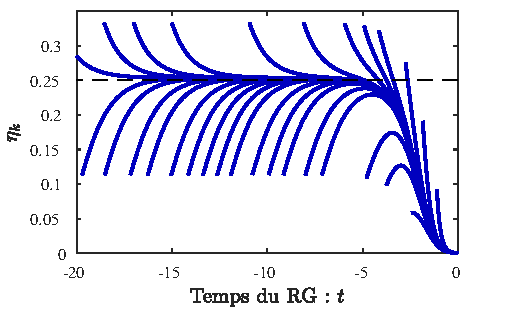
\includegraphics[width=0.95\columnwidth]{etakd2.pdf}
		\caption{(La courbe se lit de droite à gauche) Évolution de $\eta_k$ en fonction de $t= \ln(k/\Lambda)$ pour différentes étapes de la dichotomie sur $\tilde{r}_0$. En pointillés noirs nous avons représenté la valeur exacte attendue $\eta = 0.25$. }
		\label{fig:etakd2}
	\end{center}
\end{figure}
\vspace*{-20pt}
Après être passées par ce quasi-plateau les courbes divergent (en partant soit vers le haut, soit vers le bas). Ceci s'explique par le fait que nous n'avons pas trouvé avec une précision infinie la valeur de $\tilde{r}_0$ correspondant à la température critique. De ce fait n'étant pas parfaitement au point critique mais très proche on peut montrer que les courbes s'écartent du quasi-plateau en $\simeq \pm \exp(-t/\nu)$ où $\nu$ est l'exposant critique. Nous avons donc pu retrouver, pour $N=1, d =2$, la valeur
\begin{equation}
	\eta = 0.253 %\quad \text{et} \quad \nu = 1.01
\end{equation}

Ces résultats sont ceux qui avaient déjà été trouvé avec le même code (que nous avons réorganisé). C'est une valeur en bon accord avec la valeur théorique : $\eta = 0.250$.  \\




\subsection{Résultats pour $(N = 2,3, d=2)$}


Nous nous sommes par la suite intéressé au cas $N>1$. Nous savions que le code donnait de bons résultats pour les configurations $N = 2$ et $N=3$ à $d=3$. Nous nous sommes donc ensuite plus particulièrement intéressé au cas $N = 2$ et $N=3$ pour $d = 2$. Nous savions que le code ne fonctionnait, en revanche, pas avec ces paramètres. Nous avons essayé de trouver et résoudre les problèmes. Pour cela, à $N=2,3$ fixé, nous avons repris les conditions initiales de l'équations menant à un quasi-plateau pour $d=3$ et nous avons cherché un quasi-plateau en $d= 2.9$ en utilisant des conditions initiales très proches. Nous avons ensuite utilisé le résultat obtenu avec $d = 2.9$ pour une valeur de $d < 2.9$ et ainsi de suite nous avons fait descendre $d$ par petits pas jusqu'à trouver des irrégularités. \\

 La première difficulté que nous avons rencontré lors de ces simulations a été la présence probable d'un pôle dans l'expression du propagateur $G_k(q, \rho)$ en $(q = 0, \rho = 0)$ qui se trouve être intégré dans les expressions de $\tI$ et $\tJ$. En effet il semblerait que plus on descend en dimension (i.e. plus on se rapproche de $d=2$) plus la discrétisations numériques de $G_k(q, \rho)$ se rapproche de ce pole à partir d'une certaine étape de la résolution. Ce pôle n'apparait cependant que pour certaines conditions initiales (i.e. $\tilde{r}_0, \tilde{u}_0$) mais il provoque des instabilités qui peuvent nous empêché d'observer un quasi-plateau de $\eta_k$. La deuxième difficulté à été le temps à partir duquel il était possible d'apercevoir un quasi-plateau. En effet ce temps augmentait pour des valeurs de $d$ inférieures à $2.5$ - $2.4$ (alors que pour $d=3$ il fallait attendre $t<-5$ il fallait ici attendre $t<-8$ ou moins). \\
 
 Pour tenter de corriger les problèmes nous avons fait varier le nombre de points d'intégration, la taille de la grille de discrétisation en champ $\rho$ ou encore $\alpha$, la constante multiplicative devant le régulateur. Cependant nous n'avons trouvé aucun changement de comportement des résultats.\\
\indent
Pour $N=3$ nous avons pu obtenir des quasi-plateaux pour $d$ compris entre $3$ et $2.3$ seulement. Cependant il s'avère que  pour $d$ proche de $2.3$ ces quasi-plateaux ne donnent pas des résultats cohérents. En effet, si l'on essaye de déterminer $\eta$, la valeur obtenue se trouve être suffisamment loin de l'intervalle de valeur dans lequel on l'attend pour considérer que le calcul n'est pas bon. De manière surprenante, des calculs faits avec des méthodes d'approximations plus drastiques que l'approximation BMW donnent de bien meilleurs résultats pour un même $d$.\\
\indent
Pour $N=2$ nous avons eu le même problème avec l'observation de quasi-plateaux ne correspondant pas à des résultats cohérents pour $2.1 < d < 2.5$. Nous avons tout de même avancé dans l'étude. En effet, en modifiant l'intervalle numérique d'intégration utilisé et en revoyant légèrement l'implémentation du calcul des intégrales nous avons pu obtenir des modifications de nos résultats. On obtient alors pour $d=2.1$ un quasi plateau plus proche de ce qui est attendu c.f. \refig{etakd21}, en comparaisons avec ce que l'on obtenait auparavant c.f. \refig{etakd21Bis}. Cependant, avec ce type de modifications, pour $(N=3, d=3)$ nous obtenons $\eta= 0.042$ au lieu de $\eta = 0.041$ (valeur obtenue avec le code sans modifications). La valeur théorique est $\eta = 0.040$. Pour $(N=1, d=2)$ nous trouvons de même $\eta \sim 0.26$ au lieu de $\eta \in [0.250, 0.253]$ attendu. Il serait donc possible que le calcul des intégrales soit responsable des problèmes que l'on observe même si les modifications testées peuvent aboutir à des résultats moins bons dans certaines configurations que le code sans modifications. Malheureusement les premiers essais d'améliorations n'ont pas été concluants, nous n'avons pas réussi à obtenir de quasi-plateau pour $d<2.1$. Nous n'avons pas eu le temps d'aller plus loin et de reprendre le cas $N=3$.
\begin{figure}[H]
	\begin{center}
		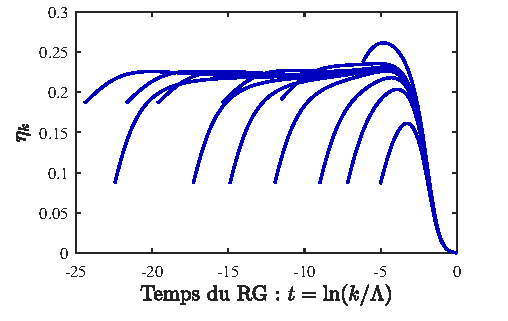
\includegraphics[width=0.95\columnwidth]{etakd21.pdf}
		\caption{(La courbe se lit de droite à gauche) Évolution de $\eta_k$ en fonction de $t= \ln(k/\Lambda)$ pour différentes étapes de la dichotomie sur $\tilde{r}_0$ pour $d=2.1$, $N=2$. Cette courbe a été obtenue après modification du calcul des intégrales. Cette courbe ne semble pas parfaite mais on peut supposer qu'elle est proche de posséder un pseudo-plateau cohérent avec ce que l'on attend $\eta \sim 0.22$. Ce pseudo-plateau n'en est peut être pas vraiment un tout de même à cause de l'effet bosselé que l'on observe en début de courbe..}
		\label{fig:etakd21}
	\end{center}
\end{figure}
\begin{figure}[H]
	\begin{center}
		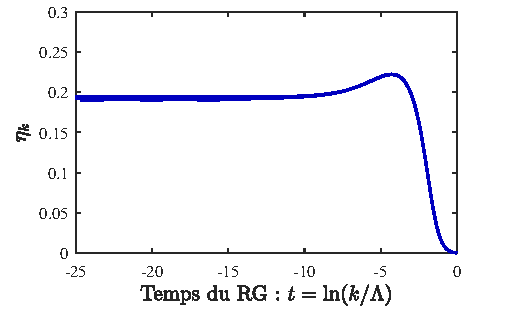
\includegraphics[width=0.95\columnwidth]{etakd21Bis.pdf}
		\caption{(La courbe se lit de droite à gauche) Évolution de $\eta_k$ en fonction de $t= \ln(k/\Lambda)$ pour différentes étapes de la dichotomie sur $\tilde{r}_0$ pour $d=2.1$, $N=2$. Cette courbe a été obtenue avant modification du code. On pourrait croire avoir un pseudo-plateau cependant celui ci n'est pas réaliste, la valeur $\eta = 0.194$ qu'il nous donnerait semble trop loin de ce qui est attendu pour $d=2.1$.}
		\label{fig:etakd21Bis}
	\end{center}
\end{figure}
\end{multicols*}



\begin{figure}[H]
	\begin{center}
		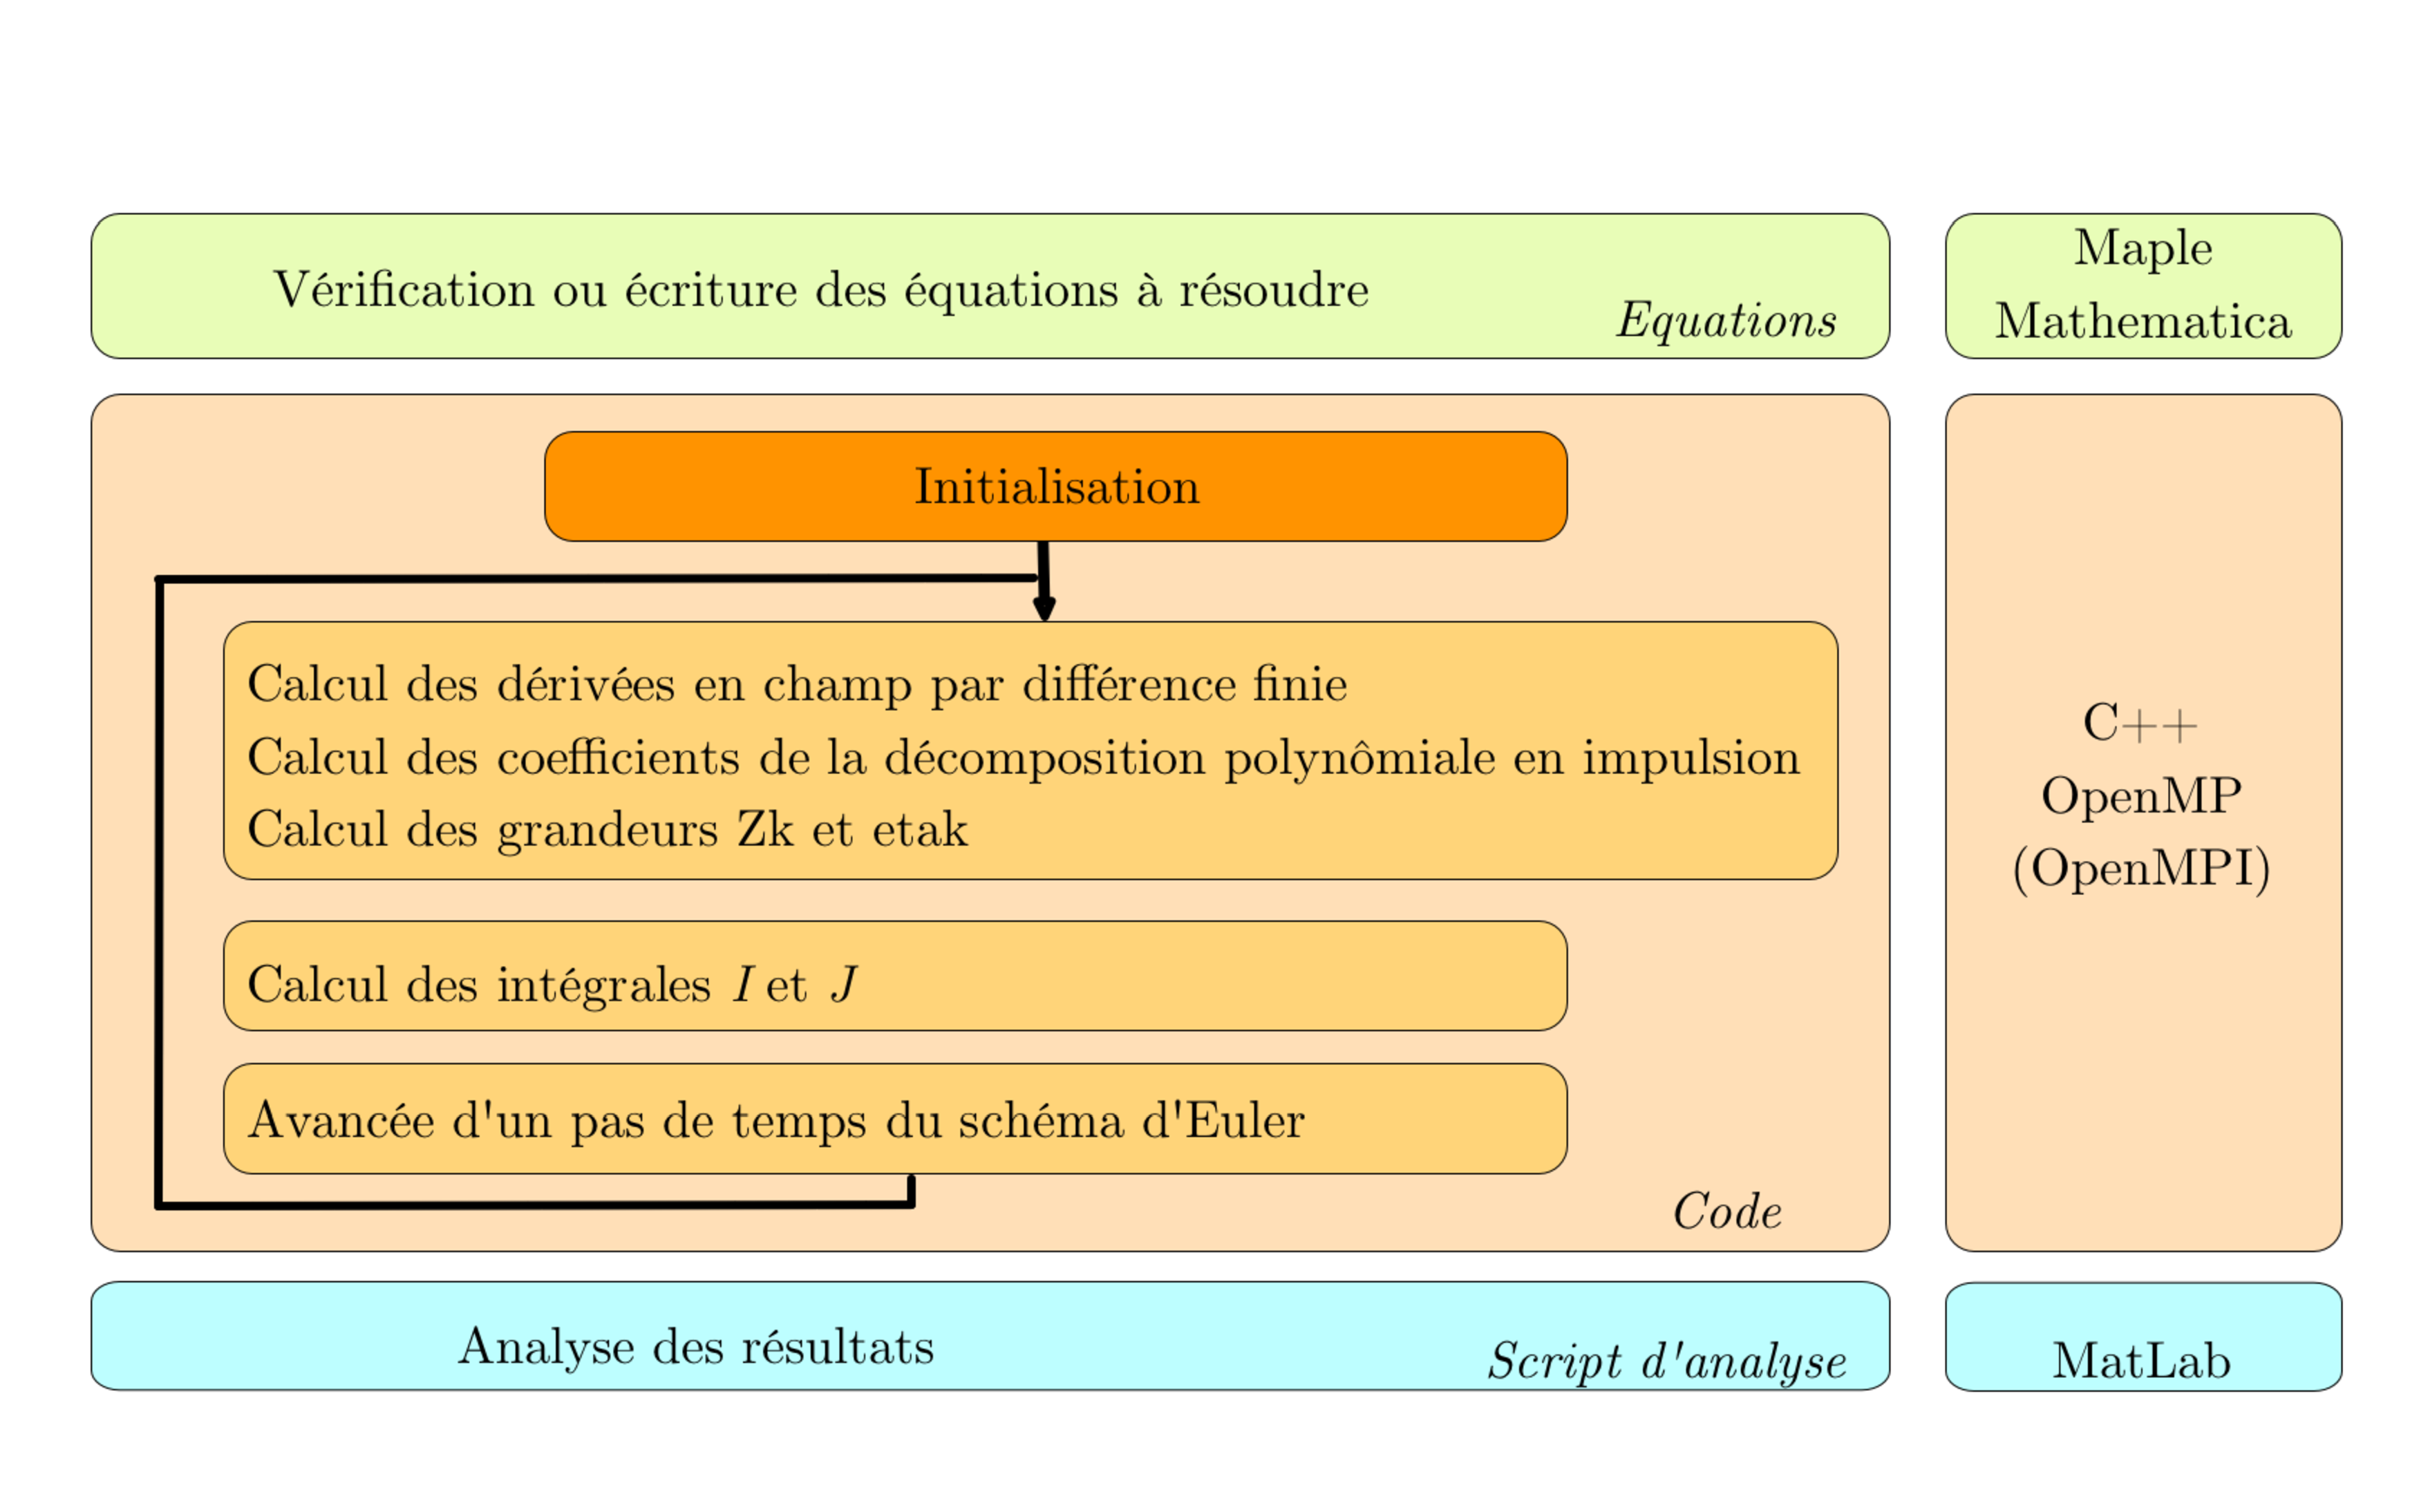
\includegraphics[width=0.95\columnwidth]{Diagramme_Code_2.pdf}
		\caption{Schéma de la répartition du travail effectué. Nous avons commencé par retrouver ou écrire les équations BMW à résoudre (vert). Ensuite nous avons réécrit ou écrit les codes C++ de simulation de ces équations ayant la structure indiquée (rouge). Toutes les parties orangées sont parallélisée sous OpenMP. Enfin nous étudions les résultats à l'aides de scripts Matlab ou Gnuplot (bleu).}
		\label{fig:org}
	\end{center}
\end{figure}

\begin{multicols}{2}


\newpage
\phantom{.}
\newpage


\section{Retour sur le modèle d'Ising 2D}

\label{sec:Ising}

Nous abordons maintenant une nouvelle étude. En effet, après nous être intéressés au calcul des exposants critiques du modèle continu $O(N)$ nous avons voulu montrer que le NPRG couplé à l'approximation BMW était une méthode suffisamment précise pour calculer des grandeurs non universelles comme la température critique de la transition de phase d'un système réaliste donné. Pour cela nous avons entrepris de calculer la température critique du modèle d'Ising 2D présenté dans l'introduction à l'aide des équations BMW. En effet il nous était facile par la suite de vérifier la qualité de l'approximation en comparant la valeur numérique obtenue à la valeur théorique calculée par Onsager \cite{Onsager}. \\

Cependant, comme nous l'avons mentionné en décrivant le formalise de la théorie des champs pour la mécanique statistique, le modèle d'Ising 2D ne satisfait pas à une description par des champs qui puisse permettre de lui appliquer le NPRG. En effet le système est décrit par des micro-états $\Mr = \{ S_\rv\}_\rv$ . Ces micro-états sont des ensembles de variables discrètes qui ne peuvent prendre que les valeurs $-1$ et $1$.  On rappelle que le hamiltonien pour $\Mr$ est alors défini par
\begin{equation}
	 H(\Mr) = -J \sum_{\left<\rv, \rv'\right>}S_\rv S_{\rv'} \, .
\end{equation}
La fonction de partition associée est la somme sur l'ensemble des micro-états possible du système 
\begin{equation}
	\Zc = \sum_{\Mr} \exp\(-\frac{H(\Mr)}{k_B T}\) \, .
\end{equation}
Nous avons donc utilisé une astuce mathématique nous permettant de
transformer la fonction de partition précédente en fonction de partition exprimé dans la théorie des champs et de la forme
\begin{equation}
\Zc = \int \Dc \varphi \exp\(-\Hc[\varphi]\) \, .
\end{equation}
Les micro-état ne sont pas décrits par des champs puisque les variables $S_\rv$ ne peuvent prendre que deux valeurs $-1$ et $1$ et ne sont pas comprises dans $\R$ tout entier. De plus elles sont définies pour des $\rv$ discrets correspondants aux positions des noeuds du réseau. Ces deux problèmes peuvent être résolus. Pour travailler avec des fonctions dans $\R$ et non $\{-1,1\}$ nous utilisons la transformée de Hubbard-Stratanovitch nous permettant de travailler avec de nouvelles variables $\varphi_\rv$ définies dans $\R$. Pour la définition en $\rv$ discrets on peut considérer que l'on extrapole par continuité les variables $\varphi_\rv$ pour tout $\rv \in \R$. Ceci revient à dire que le pas du réseau est faible devant sa taille, ce qui est justement le cas, par définition, dans la limite thermodynamique (où l'on considère un réseau de taille infinie). Cette démarche\footnote{Elle a plus précisément été faite pour un réseau d'Ising en dimension $d$ non nécessairement égale à 2.} a été réalisée dans \cite{Ising2DNPRG}. Nous l'avons détaillée en \refann{IsingChamp}. Nous présentons le résultat obetnu en section suivante. \\



\subsection{Modélisation avec des champs}




Nous montrons en \refann{IsingChamp} que la fonction de partition du modèle d'Ising 2D peut se réécrire sous la forme.

\begin{equation}
  \Zc  \propto \int_\R \prod_{\rv} \, \dd \varphi_\rv \, \exp\(-\Hc_\mu[\varphi] \) \, ,
\end{equation}
avec l'hamiltonien $\Hc_\mu$ définit par 
\begin{equation}
  \Hc_\mu[\varphi] = \frac{1}{2} \int_\qv \varphi(\qv) \frac{1}{\lambda_\mu(\qv)} \varphi(-\qv) - \sum\limits_\rv \ln\(\cosh(\varphi_\rv)\) \, ,
\end{equation}
La grandeurs $\mu$ est un réel tel que $\mu > 2J$ et $\beta = 1/(k_BT)$. Les variables $\varphi_\rv$ sont à valeurs dans $\R$ pour $\rv = m\ev_x + n\ev_y$ $(m,n) \in \N^2$. Ainsi $\rv$ est dans l'ensemble des positions des noeuds du réseau du modèle d'Ising 2D (dans lequel nous avons exprimé toutes les longueurs en unité du pas du réseau). Nous avons défini $\qv \to \varphi(\qv)$ comme une transformée de Fourier semi-discrète de $\{\phi_\rv\}_\rv$ (\refann{TFSD}) en posant, pour $\qv \in [-\pi, \pi]^2$,
\begin{equation}
  {\varphi}(\qv) = \sum_\rv \varphi_\rv e^{-i\qv\rv} \quad \text{et} \quad \varphi_\rv = \int_\qv {\varphi}(\qv)  e^{i\qv\rv}
\end{equation}
et la notation de l'intégrale sur $\qv=(q_x, q_y)$ devient
\begin{equation}
\int_\qv ... \, \equiv \, \int_{-\pi}^{\pi}	\int_{-\pi}^{\pi}	... \, \dd \, q_x \dd \, q_y
\end{equation}


Nous avons aussi introduit les fonctions
\begin{equation}
\begin{split}
	\gamma(\qv ) & = \frac{1}{2} \(\cos(q_x) + \cos(q_y)\) \\
	 \lambda_\mu(\qv) & = 2\beta\(2J \gamma(\qv) + \mu\) \, .
	 \end{split}
\end{equation}

Par isométrie de la TFSD, nous réecrivons $\Hc_\mu$ comme
\begin{equation}
  \begin{split}
    \Hc_\mu[\varphi] & = \frac{1}{2} \int_\qv \varphi(\qv) \[\frac{1}{\lambda_\mu(\qv)} - \frac{1}{\lambda_\mu(0)}\] \varphi(-\qv) \\
    &+ \sum\limits_\rv \[\frac{1}{2\lambda_\mu(0)}\varphi_\rv^2 - \ln\(\cosh(\varphi_\rv)\) \]
  \end{split}
\end{equation}
Enfin, il est aussi possible d'introduire un paramètre $\delta \in \R^+_*$ permettant de changer l'échelle du champ en posant le changement de variable, $ \varphi \rightarrow 2 \delta\sqrt{\beta J} \, \varphi $. On obtient alors l'hamiltonien sous la forme
\begin{equation}
\Hc_\mu[\varphi] = \frac{1}{2} \int_\qv {\varphi}(\qv)\eo(\qv){\varphi}(-\qv) + \sum_\rv U(\varphi(\rv)) \,,
\end{equation}
avec les notations 
\begin{equation}
  \eo(\qv) = \delta^2\frac{1 - \gamma(\qv)}{(\gamma(\qv) + \tilde{\mu})(1+\tilde{\mu})}
\end{equation}
\begin{equation}
  U(\phi) = \delta^2 \frac{1}{1+\tilde{\mu}} \frac{1}{2}\phi^2 - \ln\(\cosh\(\delta\sqrt{2\tilde{\beta}}\phi\)\) \, 
\end{equation}


\noindent
où $\tilde{\mu} = \mu/(2J)$ et $\tilde{\beta} = 2\beta J$. On retrouve ainsi la formulation d'un problème de théorie des champs que l'on peut résoudre avec le NPRG et l'approximation BMW. Concernant la mise en pratique, la seule différence avec tout ce qui a été étudié précédemment c'est qu'ici, par TFSD, les intégrales sur les moments ne sont plus calculées sur un domaine infini mais sur "la première zone de Brillouin", i.e. sur la surface $[-\pi, \pi]^2$. Comme le modèle d'Ising 2D possède une symétrie\footnote{en effet $H$ est invariant par l'échange de $\ev_z$ en $-\ev_z$ comme nous avons pu le voir dans l'introduction. \\
On peut même voir que aussi directement que $\Hc_\mu[-\varphi] = \Hc_\mu[\varphi]$.} $\mathbb{Z}_2$, l'équation de flot BMW \refeq{flotBMW} pour la symétrie $\mathbb{Z}_2$ reste valable en prenant en compte cet ajustement.\\

La fonction $U$ représente ce que l'on appelle le potentiel du système dans l'approximation de champ moyen. Le potentiel effectif $V_k(\phi)$ prend en $k=\Lambda$ la valeur $V_\Lambda = U$. La fonction $\eo$ s'appelle la relation de dispersion. Dans le modèle continu $\varphiv^4$ il y avait de même une relation de dispersion que nous n'avions pas pris la peine d'expliciter car elle valait alors $\varepsilon(\pv) = \pv^2$.\\
 
Enfin, la recherche de point fixe pour se système se fait en variant le paramètre directement lié à la température $\tilde{\beta}$ dans les conditions initiales. On cherche donc $\tilde{\beta}_c = 2d/(k_BT_c)$ pour lequel les équations dimensionnées écrites plus loin possède un point fixe. Un point fixe ne pouvant être trouvé qu'à la température critique, de cette manière on obtient la température critique.\\



\subsection{Régulateur}

La présence de la relation de dispersion $\eo$ dans $\Hc_\mu$ nous contraint, pour satisfaire à toutes les conditions d'un régulateur du NPRG qui soit $\Cc^\infty$, à utiliser
\begin{equation}
	\Rc_k(\qv) = \alpha \frac{\eo(\qv)}{\exp{(\eo(\qv)/\varepsilon_k)} -1}
\end{equation}
Avec $\varepsilon_k = \| \eo \|_\infty k^2$. Les expressions de la dérivées $\partial_t \Rc_k$ se trouvent en \refann{Ising2D}. 
\begin{figure}[H]
\begin{center}
	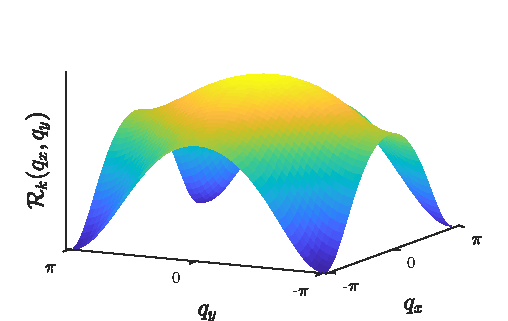
\includegraphics[width=0.8\columnwidth]{RegIsing.pdf}
\end{center}
\caption{Allure du régulateur choisi pour une valeur de $k\simeq 1$.}
\end{figure}



\subsection{Les 3 étapes de la résolution}

Pour des raisons pratiques nous avons décomposé la résolution numérique des systèmes d'équations BMW du modèle d'Ising en 3 étapes, en procédant à un adimensionnement progressif des équations. L'adimensionnement est en effet nécessaire pour pouvoir trouver une solution de point fixe et déterminer la température critique avec précision. Cependant le caractère de \textit{solution de point fixe} est une notion asymptotique pour $k \to 0$ comme nous avons pu le voir. Il est donc possible de commencer par résoudre des équations non adimensionnées qui offrent des avantages pour le calcul numérique et de passer vers des équations adimensionnées seulement à partir d'un certain temps $t$ (i.e. d'un certain $k$). \\

L'équation \refeq{flotBMW} donne alors les trois jeux d'équations BMW pour le système Ising 2D suivant que nous avons cherché à résoudre.



\subsubsection{Première étape}

En écrivant le système d'équation BMW \textit{dimensionné}, directement issu de \refeq{flotBMW} toutes les fonctions inconnues sont $2\pi$ périodiques selon les composantes des moments (ce qui ne serait plus le cas dans un système dimensionné). Cette propriété permet de s'affranchir de certaines approximations numériques dans le calcul des intégrales $J_n$ apparaissant dans les équations BMW. Il est donc préférable de commencer par résoudre ce système, que l'on note $(\Ec_1)$, sans réaliser d'adimensionnement pour $k$ variant de $\Lambda$ à $k_a$ (où $k_a \in ]0, 1]$ est une valeur que l'on va décrire plus loin). Le problème BMW ($\Pc_1$) à résoudre est donc \\

\noindent
{\itshape Trouver $(\Delta_k$, $X_k)$, solution de $(\Ec_1)$, i.e tels que pour tout $p_x \in [-\pi, \pi]$, $p_y \in [-\pi, \pi]$, $\phi \in \R$, $k\in [k_a, \Lambda]$}


\begin{align}
	\partial_t  \Delta_k (p_x, p_y, \phi) & = 
	\begin{aligned}[t]
	&  J_3(p_x, p_y, \phi) \partial_{\phi} \left\{ \Delta_k (p_x, p_y, \phi) + X_k(\phi) \right\} \\
	&  - \frac{1}{2} I_2(\phi) \partial_{\phi}^2 \Delta_k(p_x, p_y, \phi) \\
	& - I_3(\phi){(\partial_{\phi} X_k(\phi))}^2
	\end{aligned}
	\label{eqn} \\
	\partial_t X_k(\phi) & = 
	\begin{aligned}[t]
		& \frac{1}{2} \partial_{\phi}^2 I_1(\phi) \, ,
	\end{aligned}
\end{align}
où l'on note $X_k(\phi) = \partial_{\phi}^2 V_k(\phi)$. Les notations $J$ et $I$ correspondent à celle du modèle $\varphiv^4$ et leurs expressions sont écrites en \refann{Ising2D}. \\


Les conditions initiales de ce problème viennent de la condition initiale générale des équations BMW \refeq{initFlotBMW} et de la relation $X_\Lambda(\phi) = \partial_\phi^2 U(\phi)$,
\begin{equation}
	\Delta_\Lambda = 0 \quad \text{et} \quad X_\Lambda(\phi) =  \delta^2 \frac{1}{1+\tilde{\mu}} - \frac{2\delta^2\tilde{\beta} }{\cosh^2\(\delta\sqrt{2\tilde{\beta}}\phi\)}
\end{equation}



\subsubsection{Deuxième étape}



Dans un second temps, alors que $k$ devient relativement faible (i.e. inférieur à la valeur $k_a<1$ introduite précédemment), malgré la mise à profit de la périodicité des fonctions, nous rencontrons des problèmes de précision dans le calcul des intégrales numériques $I_n$ et $J_n$ qui apparaissent dans le système $(\Ec_1)$. Or $k$ n'est alors pas assez faible à ce moment de la résolution pour pouvoir passez à un système totalement adimensionné car cela nécessite d'autres approximations que l'on ne peut pas faire.  On utilise alors un nouveau système d'équations $(\Ec_2)$ dans lequel nous avons adimensionné les moments. En fait ceci correspond seulement à écrire les équations en fonction de $\tilde{\pv} = (\tp_x, \tp_y) = \pv/k = (p_x/k, p_y/k)$ (ou $\tqv = \qv/k$) au lieu de $\pv$ (ou $\qv$). Ces nouvelles équations prennent pour conditions initiales le résultats de la résolution numérique de $(\Ec_1)$ en $k = k_a$. \\

\begin{figure}[H]
\begin{center}
	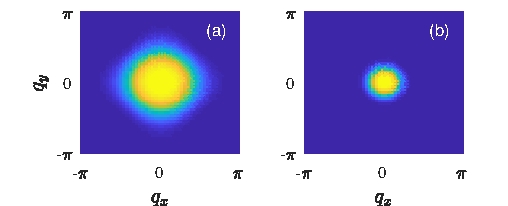
\includegraphics[width=0.95\columnwidth]{DerRegIsing.pdf}
	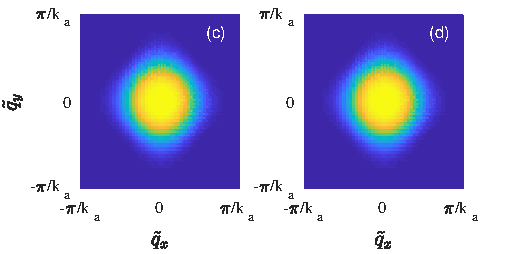
\includegraphics[width=0.95\columnwidth, height = 0.4\columnwidth]{DerRegIsing2.pdf}
\end{center}
\caption{(a-b) Représentation  de $(k, q_x, q_y) \to \partial_t \Rc_k(q_x, q_y)$ pour deux valeurs de  $k$ notées $k_1$ (a) et $k_2$ (b) sur la boite/le carré de discrétisation en moments $[-\pi, \pi]^2$. Nous avons choisi $k_1>k_2$. On représente en fait la zone utile d'intégration dans $[\pi, \pi]^2$. En effet plus la couleur est bleue foncée plus la fonction est proche de 0. Ainsi on peut considérer que seule la partie dans la tache jaune contribue réellement à la valeur des intégrales, ailleurs la fonction est "quasi-nulle". (c-d) Représentation de $(k, \tq_x, \tq_y) \to \partial_t \Rc_k(k\tq_x, k\tq_y)$ dans la boite $[-\pi/k_a, \pi/k_a]^2$ pour  $k_1$ (c) et $k_2$ (d) en ayant choisi ici $k_a = k_1$. Même si $k_1>k_2$ toujours, il n'y a plus d'évolution de la zone utile d'intégration avec les nouvelles variables adimensionnée $\tq_x$ et $\tq_y$.}
\label{fig:DerRegIsing}
\end{figure}

En effet les expressions $I_n$ et $J_n$ on la forme
\begin{equation}
	I_n, J_n \propto \int_{-\pi}^{\pi}  \int_{-\pi}^{\pi} \partial_t \Rc_k(q_x, q_y)\times ... \, \dd \, q_x \, \dd \, q_y \, .
\end{equation}
Or pour un $k < k_a$ suffisamment faible la fonction $(k,\qv) \to \partial_t \Rc_k(\qv)$ possède une valeur non négligeable sur une zone de $[-\pi, \pi]^2$ qui est d'autant plus recentrée autour de l'origine que $k$ est faible. Ainsi pour $k$ décroissant la surface d'intégration réellement utile diminue (c.f. \refig{DerRegIsing}). Ceci pose des problèmes de précision dans le calcul des intégrales quand on travaille avec une quadrature possédant un nombre de point fixé. Autrement dit, l'espacement des points de la quadrature ne correspond plus à l'échelle de variation des fonctions à intégrer\footnote{Seuls les points d'intégration présents dans la zone où $\Rc_k(\qv)$ possède une valeur non négligeable (zone jaune orange de \refig{DerRegIsing}) apportent une contribution à l'intégrale.}. \\
\indent
Poser $\tilde{\pv} = \pv/k$ est équivalent à construire une boite numérique de discrétisation en moments \textit{dynamique} dont les dimensions diminuent au fur et à mesure que $k$ diminue vers $0$, tout ceci avec un nombre de points d'intégration constant\footnote{La nouvelle boite de discrétisation en $\tpv$ est définie par $[-\tp_{max}, \tp_{max}]^2$ ce qui correspondrait, pour la variable $\pv= k\tpv$, à une boite de dimension $[-k\tp_{max}, k\tp_{max}]^2 \subset [-\pi, \pi]^2$, diminuant avec $k$.}.


On peut alors définir enfin $k_a$ de manière à ce que $(k,\tqv) \to \partial_t \Rc_k(k\tqv)$ ne soit quasi-nulle que sur les bords la nouvelle boite de discrétisation en $\tqv$ pour tout $k \le k_a$. On conserve ainsi une précision de calcul constante à faible $k$. Ceci modifie tout de même les équations et le problème ($\Pc_2$) à résoudre devient \\


\noindent
{\itshape Trouver $(\bDelta_k$, $\bX_k)$, solution de $(\Ec_2)$, i.e tels que pour tout $\tp_x \in [-\tp_{max}, \tp_{max}]$, $\tp_y \in [-\tp_{max}, \tp_{max}]$, $\phi \in \R$, $k\in [k_b, k_a]$}

\begin{align}
	\partial_t  \bDelta_k (\tp_x, \tp_y, \phi) & = 
	\begin{aligned}[t]
	&  \bJ_3(\tp_x, \tp_y, \phi) \partial_{\phi} \left\{ \bDelta_k (\tp_x, \tp_y, \phi) + \bX_k(\phi) \right\} \\
	&  - \frac{1}{2} \bI_2(\phi) \partial_{\phi}^2 \bDelta_k(\tp_x, \tp_y, \phi) \\
	& - \bI_3(\phi){(\partial_{\phi} \bX_k(\phi))}^2 \\
	& + \tp_x \partial_{\tp_x} \bDelta_k (\tp_x, \tp_y, \phi)  \\
	& + \tp_y \partial_{\tp_y}  \bDelta_k (\tp_x, \tp_y, \phi) 
	\end{aligned}
	\label{eqn} \\
	\partial_t \bX_k(\phi) & = 
	\begin{aligned}[t]
		& \frac{1}{2} \partial_{\phi}^2 \bI_1(\phi)
	\end{aligned}
\end{align}
On pourra se référer à \refann{Ising2D} pour les différentes notations. Les conditions de raccordement sont
\begin{equation*}
\bDelta_{k_a}(\tp_x, \tp_y, \phi) = \Delta_{k_a}(p_x, p_y, \phi) \quad \text{et} \quad \bX_{k_a}(\phi) = X_{k_a}(\phi)
\end{equation*}

Pour assurer la compatibilité entre les deux systèmes il faut alors respecter $k_a\tp_{max} = \pi$. \\




\subsubsection{Troisième étape}

On utilise enfin, dans un dernier temps, un nouveau système $(\Ec_3)$ adimensionnées qui va nous permettre de trouver une \textit{solution de point fixe} et par la même occasion de déterminer la température critique. Ce système met en jeu des approximations que nous ne pouvions pas réaliser sans avoir $k < k_b$ avec $k_b$ suffisamment faible. On prend comme condition initiale le résultat donné par la simulation de $\Ec_2$ à $k = k_b$. Le problème se transforme en ($\Pc_3$), \\

\noindent
{\itshape Trouver $(\tY_k$, $\tX_k)$, solution de $(\Ec_3)$, i.e tels que pour tout $\tp_x \in [-\tp_{max}, \tp_{max}]$, $\tp_y \in [-\tp_{max}, \tp_{max}]$, $\tphi \in \R$, $k\in ]0, k_b]$}

\begin{equation}
\begin{split}
\partial_t & \tY_k(\tp_x, \tp_y,\tphi)  = \eta_k(1+\tY_k(\tp_x, \tp_y,\tphi)) \\
& + \frac{1}{2} \eta_k \tphi \partial_{\tphi} \tY_k(\tp_x, \tp_y,\tphi) - \frac{1}{2} \tI_2(\tphi) \partial_{\tphi}^2 \tY_k(\tp_x, \tp_y, \tphi) \\
&  + \frac{1}{\eo^0\tpv^2}\left\{ {\( \eo^0\tpv^2 \partial_{\tphi} \tY_k(\tp_x, \tp_y,\tphi) + \partial_{\tphi} \tX_k(\tphi)\)}^2 \tJ_3(\tp_x, \tp_y,\tphi) \right.\\
& \left. - {\( \partial_{\tphi} \tX_k(\tphi) \)}^2 \tI_3(\tphi)\right\} \\
& + \tp_x \partial_{\tp_x} \tY_k(\tp_x, \tp_y,\tphi) + \tp_y \partial_{\tp_y} \tY_k(\tp_x, \tp_y,\tphi),
\end{split}
\end{equation}
\begin{equation}
\partial_t \tX_k(\tphi)  = (\eta_k -2)\tX_k(\tphi) + \frac{1}{2}\eta_k\tphi \, \partial_{\tphi}\tX(\tphi) + \frac{1}{2} \partial_{\tphi}^2 \tI_1(\tphi)
\end{equation}
\textit{avec la définition}
\begin{equation}
\eta_k = \frac{1}{2} \tI_2(0) \partial_{\tphi}^2 \tY_k(0,0,0) \, .
\end{equation}
On pourra ici aussi se référer à \refann{Ising2D} pour les différentes notations et plus de précision. Avec les notations utilisée les conditions de raccordement sont 
\begin{equation*}
\tY_{k_b}(\tp_x, \tp_y,\tphi) = \frac{1}{Z_k}\( 1+ \frac{\bDelta_{k_b}(\tp_x, \tp_y, \phi)}{\eo^0 k_b^2(\tp_x^2 +\tp_y^2)}\) -1
\end{equation*}
\begin{equation*}
\tX_{k_b}(\tphi) = \frac{1}{Z_kk^2}\bX_{k_b}(\phi)\, .
\end{equation*}
 
De même que dans les équations du modèles $\varphiv^4$ si l'on trouver une solution de point fixe alors $\eta_k^*$ associée vérifie $\eta = \eta_{k \to 0}^*$ et on détermine l'exposant $\eta$ recherché ainsi. \\

En conclusion l'important ici est cette résolution numérique des équations que l'on découpe en trois problèmes $(\Pc_1)$,  $(\Pc_2)$ et $(\Pc_3)$ distincts (associés au systèmes d'équations $(\Ec_1)$,  $(\Ec_2)$ et $(\Ec_3)$) pour conserver une précision maximale lors de la résolution numérique. On remarque aussi que comme dans le modèle continu $\varphiv^4$, l'équation de flot BMW \refeq{flotBMW} ne possédant pas de conditions au bords, nos équations n'en possèdent pas non plus.\\



\section{Méthodes et outils numériques pour la résolution d'Ising 2D}

\label{sec:NumIsing}
Nous allons passer en revue et justifier ici les principales méthodes numériques que nous avons mises en œuvre pour tenter de résoudre les systèmes d'équations précédents. En grande partie nous avons repris la méthodologie générale utilisée pour la résolution du modèle continu $\varphiv^4$.


\subsection{Structure du code}

Pour la discrétisation en \textit{temps du RG} $t$ le plus simple a été de conserver un schéma d'Euler explicite à cause de la non-linéarité des équations. Nous n'avons pas utilisé de schéma de Rung-Kutta car de manière générale le schéma d'Euler s'est avéré efficace.\\

La différence principale entre les équations du modèle continu $\varphiv^4$ et ces nouvelles équations est qu'ici pour les dimensions de moments les fonctions ne dépendent plus seulement de $p$ (i.e. la norme de $\pv$) mais de ses deux composantes $p_x$ et $p_y$. Le plus gros défit dans la simulation est en fait de calculer les intégrales $J, \bJ, \tJ$ apparaissant respectivement dans $(\Ec_1)$, $(\Ec_2)$ et $(\Ec_3)$. En effet, pour $n\in\N^*$ $J_n$, par exemple, s'exprime comme 
\begin{equation}
	J_n(p_x, p_y, \phi) = \int_\qv u(q_x+p_x, q_y+p_y, \phi) h(q_x,q_y, \phi) \, ,
\end{equation}
où $u$ et $h$ sont des fonctions de $\Delta_k$ et $X_k$. Les sommes $p_x+q_x$ et $p_y+q_y$ sont un gros problème pour l'intégration numérique. En effet il est nécessaire de calculer l'intégrale, à tout pas de temps $t$, pour tout $\phi$ et pour tout $p_x$ et $p_y$ de la discrétisation en moments. De plus il faut pouvoir trouver une quadrature réalisant ce calcul avec précision. Ainsi nous avons conservé le choix de réaliser des intégrations avec la méthode de Gauss-Legendre. Ceci nécessite de discrétiser les fonctions inconnues $\Delta_k$, $\bDelta_k$,$X_k$, ... selon les variables de moment avec une méthode d'interpolation pseudo-spectrale. Nous avons utilisé une méthode d'interpolation sur les polynômes de Tchebytchev. La difficulté a résidé en la réécriture des méthodes à une dimension (i.e. pour des fonctions d'une variable de moment $p$) déjà utilisées dans le modèle $ \varphiv^4$ en des méthodes à deux dimensions, pour des fonctions de deux variables de moment $(p_x, p_y)$. 

Une alternative aurait été d'utiliser une discrétisation des variables de moment $(p_x, p_y)$ sur une grille en deux dimensions de points régulièrement espacés. Il est alors possible d'écrire une quadrature qui permet de calculer $J$, $\bJ_3$ et $\tJ_3$ avec des algorithmes de faible complexité (en comparaison de la méthode par interpolation de Tchebytchev et quadrature de Gauss-Legendre). Cependant les quadratures alors testées\footnote{basées sur une triangulation régulière de l'espace et des descriptions des fonctions par éléments finis} demandaient un nombre trop important de points de discrétisation pour obtenir des précisions suffisantes en des temps de calculs raisonnables et elles restaient, de manière générale, moins pratiques que la méthodes d'interpolation. \\


Enfin, pour la discrétisation en champ nous avons privilégié la variable $\phi$ dans les équations et non pas $\rho = \phi^2/2$ que nous avions utilisé pour le modèle continu $\varphiv^4$ à cause de différents problèmes numériques. Nous avons toutefois conservés sur une discrétisation par une grille fixe et des calculs de dérivées par rapport à $\phi$ à l'aide de schémas aux différences finies à 5 points. \\



Ce nouveau code est donc structuré de la même manière que le code du modèle continu $\varphiv^4$. En effet, avoir réécrit le code de la simulation du modèle continu $\varphiv^4$ en C++ de façon modulable à l'aide de classes nous a permis, de manière générale, de reprendre ou d'adapter beaucoup des fonctions numériques. Pour avoir une vue générale de la structure il est donc possible de se reporter encore à la figure \refig{org}. Nous détaillons, maintenant dans la prochaine section les problèmes que l'on a pu rencontrer dans l'écriture des codes de simulations ainsi que les techniques retenues qui ont fonctionné et leurs avantages comparés à celles qui ont échoué. Nous présentons ensuite les différentes techniques plus en détails. 





\subsection{Problèmes rencontrés}

\label{sec:Problemes}

Tout d'abord nous avions écrit les équations en utilisant la variable $\rho = \phi^2/2$ pour résoudre $(\Pc_1)$. Cependant nous avons pu observer des instabilités dans le calcul des dérivées en $\rho$ pour $\rho = \rho_{max}$ (avec $\rho_{max}$ la limite supérieure de la grille de discrétisation en $\rho$). Nous avons réussi à résoudre le problème en descendant en ordre dans les schémas de calcul des dérivées en passant d'un ordre 5 à l'ordre 3. Cependant nous avons ensuite rencontré des instabilités au niveau du calcul des dérives $\partial_{\rho}$ autour de $\rho = 0$. Pour régler le problème nous avons alors utilisé la variable $\phi$. En effet il apparait alors des propriétés de parité des fonctions qui nous ont permis de donner des valeurs exactes aux dérivées en $\phi = 0$ (i.e. $\rho = 0$) et résoudre le problème. En outre la variable $\phi$ nous a aussi permis de repasser avec des dérivées en champs à 5 points sans difficultés pour $\phi = \phi_{max}$. 

Le deuxième type de problème que nous avons rencontré a été la précision de l'interpolation et du calcul des intégrales. En effet, pour trouver un point fixe il faut regarder la solution des équations BMW pour des $k$ très proches de 0. Or le découpage en trois des équations pour conserver un maximum de précision dans nos calculs ne peut pas se faire n'importe comment. Il s'avère que pour résoudre $(\Pc_1$) nous avons rencontré des problèmes de précisions dans le calcul des intégrales avant de pouvoir passer à $(\Pc_2)$. Ceci nous a imposé d'utiliser un nombre de point d'interpolation et d'intégration supérieur à ce que nous utilisions en premier lieu et de trouver de meilleures techniques pour cela. 



\subsection{Symétries et périodicité des fonctions}

\label{sec:Sym}

Commençons par étudier les symétries du problème. On note $(t_1, t_2, ..., t_n, ...)$ les temps discrets de la résolution par la méthode d'Euler. Considérons le schéma semi-discrétisé en temps associé de $(\Ec_1)$  :
\begin{equation}
	\begin{split}
	\frac{\Delta_{k_{n+1}} - \Delta_{k_{n}}}{\delta t}	& =  - \frac{1}{2} I_2(\phi) \partial_{\phi}^2 \Delta_{k_n}(p_x, p_y, \phi)  +  ... \\
	\frac{X_{k_{n+1}} - X_{k_{n}}}{\delta t} & = \frac{1}{2} \partial_{\phi}^2 I_1(\phi) \, .
	\end{split}
\end{equation}
On note $\delta t$ le pas de discrétisation en temps. On note $\Delta_{k_n}$ la fonction semi-discrétisée égale à $\Delta_k$ au temps discret $t_n$ ($k_n = \Lambda\exp(t_n)$), et de même $X_{k_n}$. Alors, par les symétries de la relation de dispersion et du potentiel $U$ initial (\refann{Sym}), la fonction $\Delta_{k_n}$ est paire selon toutes ses variables (par exemple, $\Delta_{k_n}(-p_x, p_y, \phi) = \Delta_{k_n}(p_x, p_y, \phi)$. De plus il y aussi la symétrie supplémentaire $\Delta_{k_n}(p_y, p_x, \phi) = \Delta_{k_n} (p_x, p_y, \phi)$. En outre, $X_{k_n}$ est aussi une fonction paire. 

\begin{figure}[H]
\begin{center}
	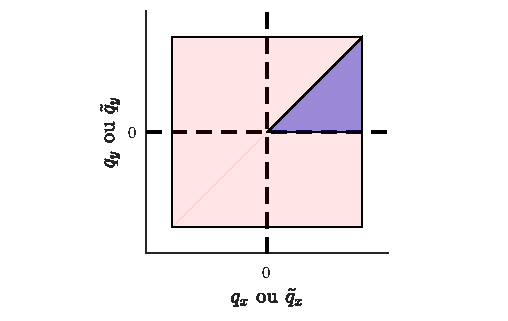
\includegraphics[width=0.95\columnwidth]{SurfUtile.pdf}
\end{center}
\vspace*{-22pt}
\caption{(rouge transparent) Zone complète sur laquelle il faudrait définir les fonctions sans symétrie. (bleue) Zone dans laquelle il suffit de définir numériquement les fonctions. Les symétries permettent de "réduire" le problème à une surface restreint de moments.}
\label{fig:SurfUtile}
\end{figure}


Ces propriétés se transmettent aux fonctions inconnues des problèles $(\Pc_2)$ et $(\Pc_3)$ que sont $\bDelta_{k_n}$, $\tY_{k_n}$, $\bX_{k_n}$ et $\tX_{k_n}$ tout naturellement grâce aux conditions de raccordement.
De cette manière on ne considère que $\phi \text{ (ou } \tphi) \in [0, \infty[$ ainsi que des moments définies sur une zone restreinte de $[-\pi, \pi]^2$ pour les fonctions inconnues de ($\Pc_1$), ou de $[-\tp_{max}, \tp_{max}]^2$ pour celles de ($\Pc_2$) ou ($\Pc_3$). On détaille plus précisément en \refig{SurfUtile} quelles sont ces zones. \\
\indent
 Enfin mentionnons que puisque $\eo$ est une fonction $2\pi$-périodique alors $\Delta_{k_n}$ l'est aussi pour tout $n\in\N$ par rapport au variables $p_x$ et $p_y$. Cette propriété est utile pour le calcul des intégrales $J_n$ comme nous le détaillerons plus précisément en \refsec{IntJ} mais elle est perdue pour les fonctions $\bDelta_{k_n}$ et $\tY_{k_n}$. C'est elle qui justifie le passage par des équations dimensionnées et le problème $(\Pc_1)$ dans les trois étapes de la résolution.





\subsection{Interpolation de Tchebytchev}

Nous souhaitons calculer avec précision les expressions $J$, $\bJ$, $\tJ$ qui sont des fonctions dépendant de moments $(p_x, p_y)$ ou ($(\tp_x, \tp_y)$) et qui s'expriment comme les intégrales sur $q_x$ et $q_y$ de $(q_x, q_y) \to u(q_x + p_{x}, q_y + p_{y})h(q_x, q_y)$, avec $u$ et $h$ des expressions dépendant de nos fonctions inconnues $\Delta_k, \bDelta_k, W_k$, etc. Pour cela avons choisi d'interpoler la partie dépendante des moments $(p_x, p_y)$ ou ($(\tp_x, \tp_y)$) des fonctions inconnues afin d'utiliser une quadrature précise des intégrales. Comme annoncé, pour cela nous réutilisons encore une interpolation de Tchébytchev adaptée en dimension 2. 

\subsubsection{Décomposition}

Nous rappelons ici une propriété justifiant l'utilisation des polynômes de Tchebytchev comme polynômes d'interpolation en dimension 2.\\

\noindent
\textbf{Décomposition de Tchebytchev 2D.} 
{\itshape  Soient $a$, $b$ deux réels tels que $b>a$. Soit $f : [a,b]^2 \rightarrow \R$ une fonction continue aux variations bornées (comme définies en \cite{Tchebychev}). On suppose que l'une des dérivées partielles de $f$ existe et est bornée dans $[a,b]$. Alors il existe une suite des coefficients réels $\{c_{ij}\}_{(i,j) \in \N^2}$ tels que la série $f_n$ définie par :
\begin{equation}
\begin{split}
f_n(x,y) = \sum_{i=0} ^{n} \sum_{j=0} ^{n} c_{ij} T_i\(\frac{2x-a-b}{b-a}\)T_j\(\frac{2y-a-b}{b-a}\)
\end{split}
\end{equation}
converge uniformément vers $f$ quand $n \rightarrow +\infty$.}\\


Ce théorème et sa démonstrations se trouvent dans l'ouvrage \cite{Tchebychev, mason1980near} dans le cas $a=-1$, $b=1$. La généralisation à $a$ et $b$ ($b>a$) quelconques est immédiate. Par la présence du régulateur qui est $\Cc^\infty$ nous travaillons, comme dans le modèle $\varphiv^4$ continu avec des fonctions de que l'on suppose très régulières. On peut alors supposer que cette propriété s'applique à nos fonctions \cite{mason1980near}. On peut, comme en \refsec{ExprCoeff} montrer que les fonctions semi-discrétisées en temps de RG $t$ du schéma d'Euler ($\Delta_{k_n}$, $X_{k_n}$, etc. introduites en \refsec{Sym}) sont régulières (au moins $\Cc^1$). 



\subsubsection{Décomposition méthode 1}

Soient $a$, $b$ deux réels ($b>a$). Soit $f$ une fonction de $[a,b]^2$ dans $\R$. Dans un premier temps nous avons opté pour un algorithme de recherche direct des coefficients $c_{ij}$ de sa décomposition en série de polynômes de Tchebytchev basée sur la méthode 1D. Supposons, en effet, que l'on veuille effectuer une décomposition à l'ordre $n_c -1$ basé sur les propriété des zéros de Tchebytchev :
\begin{equation}
  f(x,y) \simeq \sum_{i=0}^{n_c-1}\sum_{j=0}^{n_c-1} c_{ij} T_i\(\frac{2x-a-b}{b-a} \)T_j\( \frac{2y-a-b}{b-a}\)
  \label{eq:dec}
\end{equation}

Pour trouver la valeur des coefficients de la matrice $((c_{i,j}))_{i,j}$ on peut prendre les ensembles des racines du polynôme de Tchebytchev  de degré $n_c$, $\left\{x_m\right\}_{0\le m \le n_c-1}$ et $\left\{y_n\right\}_{0\le m \le n_c-1}$ et on impose \refeq{dec} en ces points, ce qui revient aussi à écrire,
\begin{equation}
\begin{split}
   f\(\frac{a+b}{2} + x_m\frac{a-b}{2}, \frac{a+b}{2} + y_n\frac{a-b}{2}\) =  \\
    \sum_{i=0}^{n_C-1} \sum_{j=0}^{n_c-1}  c_{ij} T_i\(x_m\) T_j\(y_n\)
\end{split}
\end{equation}
En utilisant les relations des polynômes de Tchebytchev on peut alors determiner les coefficients de la matrice $((c_{ij}))_{i,j}$ avec les formules
\begin{equation}
\begin{split}
 c_{ij} = & \frac{A_{ij}}{n_c^2}  \sum_{m=0}^{n_c-1}  \sum_{n=0}^{n_c-1}  T_i \(x_m\) T_j\( y_n \) \\
 & \times f\(\frac{a+b}{2} + x_m\frac{b-a}{2}, \frac{a+b}{2} + y_n\frac{b-a}{2}\)   \, ,
\end{split}
\end{equation}
avec la notation
\begin{align}
  A_{ij} = 
  \begin{cases}
    1 \quad \text{si } i = j = 0 \\
    2 \quad \text{si } i = 0 \text{ et } j \neq 0 \quad \text{ou } i \neq 0 \text{ et } j = 0 \\
    4 \quad \text{si } i \neq 0 \text{ et } j \neq 0 \\
  \end{cases}
\end{align}

Cette méthode est coûteuse puisque pour calculer l'ensemble des coefficients de $((c_{ij}))_{i,j}$ cela demande un algorithme demandant $\mathcal{O}(n_c^2)$. En outre pour ensuite obtenir $f(x,y)$ en tout point $(x,y) \in [a,b]^2$, il faut utiliser un algorithme demandant $\sim 9 n_c^2$  opérations. Afin d'obtenir de meilleurs temps de calcul sur les interpolations à précision fixée nous avons utilisé une seconde méthode.


\vspace*{11pt}

\subsubsection{Décomposition méthode 2}

\label{sec:Decomp2}

Il existe une méthode plus astucieuse que celle développée précédemment, inspirée de ce qui est mis en place dans le paquet \textit{chebfun} \cite{driscoll2014chebfun} permettant justement de traiter les interpolations de Tchebytchev sous Matlab. Cette méthode est développée dans \cite{TownsendThesis}. 

Au lieu de faire directement une décomposition sur une base tensorielle de polynômes de Chebychev on commence par réaliser une approximation de rang faible de la fonction que l'on souhaite approximer. Plus précisément, on considère les ensembles des racines de Tchebytchev noté $\left\{x_m\right\}_{0\le m \le n_c-1}$ ou $\left\{y_n\right\}_{0\le m \le n_c-1}$. On forme la matrice 
\begin{equation*}
	\mat{F} = \( \(  f\(\frac{a+b}{2} + x_m\frac{b-a}{2}, \frac{a+b}{2} + y_n\frac{b-a}{2}\)     \)  \)_{m,n}
\end{equation*}
dont on peut faire une approximation de rang faible par élimination Gaussienne avec l'algorithme suivant, en $\varepsilon$ de l'ordre de la précision machine :

\begin{algorithm}[H]
  \begin{algorithmic}[1]
    \STATE Initialisation : $\mat{E}^0 = \mat{F}$; $\mat{F}_0 = 0$; $k = 1$;
    \WHILE{ ${\| \mat{E}^k \|}_{\infty} < \varepsilon {\| \mat{E}^0 \|}_{\infty}$ }
    \STATE $(i_k, j_k) =  {\text{argmax}}_{(i,j)} \left\{\left| \mat{E}^{k-1}_{i,j} \right| \right\}$
    \STATE $\mat{C}^k_{j} = \mat{E}^k_{i_k,j}$;  $\mat{R}^k_{i} = \mat{E}^k_{i,j_k}$; $d_k = \mat{E}^k_{i_k,j_k}$
    \STATE $\mat{E}^k_{i,j} = \mat{E}^{k-1}_{i,j} - d_k^{-1}\mat{C}^k_{j}\mat{R}^k_{i}$
    \STATE $\mat{F}^k_{i,j} = \mat{F}^{k-1}_{i,j} + d_k^{-1}\mat{C}^k_{j}\mat{R}^k_{i}$
    \ENDWHILE
  \end{algorithmic}
\end{algorithm}
Notons $Q$ ($Q \le n_c$) le rang de l'approximation obtenue. La matrice $\mat{F}$ peut être approximée, à la précision machine, par  
\begin{equation}
\mat{F} \simeq \tilde{\mat{F}} = \sum_{j=1}^Q d_j \mat{C}^j \mat{R}^j \, .
\end{equation}
Comme nous ne connaissons exactement la fonctions $f$ discrétisée qu'aux points d'interpolation cela revient au même que d'écrire que nous avons décomposé $f$ comme une somme de produits de fonctions à une variable,
\begin{equation}
f(x,y) \simeq \sum_{j=1}^Q d_jc^j(y)r^j(x)
\end{equation}
et on peut décomposer les fonctions $c_j$ et $r_j$ sur une base de polynômes de Tchebytchev comme on peut le faire pour toute fonction d'une seule variable suffisamment régulière. \\


Afin de récupérer la valeur de $f$ en un point quelconque $(x,y) \in [a,b]^2 $ nous utilisons simplement la méthode de Clenshaw à une variable sur les fonctions $c^j$ et $r^j$ déjà mentionnée en \refsec{NumContinu}. Ainsi l'algorithme de décomposition possède une complexité en $\mathcal{O}(Q n_c)$ et le calcul de $f$ en $(x,y) \in [a,b]^2$ demande $\sim 6Qn_c$ opérations ($< 9n_c^2$). Le gain a eu son importance pour permettre d'atteindre des résultats convenables en des temps raisonnables. En effet nous avons pour une grande partie de la résolution $Q < n_c$ de par la régularité des fonctions et nous avons observé que cette méthode de décomposition est, de manière générale, plus rapide et plus pratique pour calculer des dérivées en moments. \\



\subsection{Le calcul des intégrales} 

Pour calculer numériquement les différentes intégrales nous nous servons des propriétés de symétrie que nous avons détaillé des fonctions inconnues. Cependant il s'est aussi posé le choix de la méthode à utiliser pour réaliser cette quadrature. Comme les intégrales sont à calculer sur une forme géométrique simple, un carré (ou la moitié d'un carré), nous avons opté pour une version "tensiorielle" d'une quadrature une dimension de Gauss-Legendre. Cependant nous avions eu d'autres idées que nous n'avons pas retenues pour diverses raisons expliquées ci-dessous.


\subsubsection{Le choix de la quadrature}

On interpole la partie en moment des fonctions avec des polynômes de Tchebytchev et on utilise toujours une méthode pseudo-specrtrale\footnote{c'est à dire que l'on connait à chaque pas de temps la valeur de la fonction aux points d'interpolation de Tchebythchev, ainsi que les coefficients de son développement en série de polynômes de Tchebytchev}. Même si nous avons choisi une quadrature de Gauss-Legendre nous nous sommes demandé si c'était vraiment la plus adaptée. En effet, pour gagner du temps et utiliser directement la connaissance des fonctions aux points d'interpolation nous avons pensé au calcul d'intégrale par la \emph{première règle de Fejer} \cite{waldvogel2006fast} (\refann{Quad}) qui permet cela.
 Cependant cette méthode s'est avérée être inefficace puisque il faut de manière générale plus de points pour obtenir la même précision qu'une quadrature de Gauss Legendre. De plus le passage le plus long du code est le calcul de $J_3$ (et ainsi que les versions adimensionnées $\bJ_3$ et $\tJ_3$) et cette quadrature ne permet pas de réaliser ce calcul plus rapidement.


%\vspace*{11pt}

\subsubsection{Calcul des intégrales $I$, $\bI$, $\tI$}

Soit $a>0$ un réel. Soit $f :(x,y) \to f(x,y)$ une fonction de $[-a, a]^2$ à valeurs dans $\R$. On suppose que $f$ est symétrique par rapport à l'axe des $x=0$, à l'axe des $y=0$ et à l'axe $x=y$. Les intégrales $I$, $\bI$ et $\tI$ sont de la forme
\begin{equation}
K = \int_{-a}^{a} \int_{-a}^{a} f(x,y) \, \dd x \, \dd y 
\end{equation} 
Pour réaliser le calcul numériquement on commence en utilisant les deux premières symétries de $f$,
\begin{equation}
K = 4 \int_{0}^{a}  \int_{0}^{a} f(x,y) \, \dd x \, \dd y \, .
\end{equation} 
Cette expression se calcule en utilisant une quadrature de Gauss-Legendre sur chaque dimension d'intégration : 
\begin{equation}
K \simeq 
 a^2\sum_{i=0}^{n_{gl}}  \sum_{j=0}^{n_{gl}}w_i w_j f(\frac{a}{2}\(\xi_i+1\), \frac{a}{2}\(\xi_j+1\)) \, ,
\end{equation}
où $\{\xi_i\}_{i \in \bbrac {1, n_{gl}}}$ sont les points de la quadrature et  $\{w_i\}_{i \in \bbrac {1, n_{gl}}}$ les poids correspondants. Par construction, $((w_i w_j))_{i,j}$ est une matrice symétrique et par symétrie de $f$ par rapport à l'axe $x=y$ nous pouvons écrire, 
\begin{equation}
\begin{split}
K \simeq a^2\sum_{i=0}^{n_{gl}} & w_i^2f(\frac{a}{2}\(\xi_i+1\), \frac{a}{2}\(\xi_i+1\)) \, + \\
 a^2\sum_{i=0}^{n_{gl}} & \sum_{j=0}^{i-1}w_i w_j 2 f(\frac{a}{2}\(\xi_i+1\), \frac{a}{2}\(\xi_j+1\)) 
\end{split}
\end{equation}
Ce qui permet de réduire le temps de calcul en réduisant légèrement le nombre d'opérations à effectuer.

\vspace*{11pt}

\commentout{
On peut alors faire le changement de variable affine  $\(\tilde{x}, \tilde{y}\) \rightarrow \(2x/a -1, 2y/a -1\) $ donnant,  
\begin{equation}
\begin{split} 
  \int_{0}^{a}  \int_{0}^{a}  f(x,y) \, & \dd x \, \dd y = \\
 \frac{a^2}{4} \int_{-1}^{1} & \int_{-1}^{1} f\(\frac{a}{2}\(\tilde{x}+1\),\frac{\pi}{2}\(\tilde{y}+1\)\) \, \dd \tilde{x}  \, \dd \tilde{y} 
\end{split}
\end{equation}
Les intégrales sur le carré unité $[-1,1] \times [-1, 1]$ sont alors calculées avec une quadrature \textit{tensorielle} obtenue à partir d'une quadrature 1D : }


\subsubsection{Calcul des intégrales $J$,$\bJ$,$\tJ$ }
\label{sec:IntJ}

Soit $a>0$. Soit $(x_0,y_0) \in [0,a]^2$. Soit maintenant $u$ et $h$ deux fonctions de $\R^2$ dans $\R$ et  $g$ définie sur $[-a, a]^2$  par $g_{x_0, y_0} : (x,y) \rightarrow u(x+x_0, y+y_0)$. On suppose que $u$ et $h$ sont symétriques par rapport à l'axe $x=0$, à l'axe $y=0$ et à l'axe $x=y$. Les intégrales $J$, $\bJ$, $\tJ$ sont de la forme 
\begin{equation}
K(x_0,y_0) = \int_{-a}^{a} \int_{-a}^{a} g_{x_0, y_0}(x,y) h(x,y) \,  \dd x \, \dd y 	 \, .
\end{equation}
En utilisant les symétries de $u$ et $h$ nous montrons que
\begin{equation}
\begin{split}
& K(x_0,y_0) = \int_{0}^{a}  \int_{0}^{a}  \left[ u(x+x_0, y+y_0) + u(x+x_0, y-y_0) \right. \\
 & +  \left. u(x-x_0, y+y_0) + u(x-x_0, y-y_0)\right] h(x,y)  \, \dd x \, \dd y 
\end{split}
\end{equation}
Et on adopte encore pour le calcul la même quadrature que pour les intégrales $I$, $\bI$, $\tI$. Cependant remarquons que ce calcul impose de connaitre les valeurs de $u$ en des points $(x \pm x_0, y \pm y_0)$ qui sont en dehors du carré $[0, a]^2$. Or, à cause de la discrétisation, $u$ est une fonction que l'on connait par sa décomposition en série de polynômes de Tchebytchev sur $[0,a]^2$ : on ne connait pas, a priori, la valeur de $u$ en tout $(x\pm x_0, y\pm y_0)$. Lorsque l'on s'intéresse au calcul de $J$ cela ne pose pas de problèmes car on peut utiliser la périodicité des fonctions (raison pour laquelle nous résolvons en premier lieu le système $(\Ec_1)$ dimensionné). En revanche, pour $\bJ$ et $\tJ$ la périodicité est brisée dans et nous sommes obligé d'extrapoler $u$ en dehors de $[0,a]^2$. 





\subsection{Dérivées numériques en champ }

Les dérivées numériques en champ $\phi$ ou $\tphi$ sont encore calculées sur 5 points pour essayer d'avoir la meilleure  précision possible. Cependant comme nous l'avons mentionné nous avons du dans des premières versions du code utilisé des dérivées sur trois points à cause d'instabilité en bords des grilles de discrétisation. Nous pouvons justifier rapidement la présence de telles instabilités. En effet, comme nous ne disposons pas de conditions aux bords pour nos équations il se trouve que nous sommes obligés d'utiliser des schémas de discrétisation à cinq points fortement décentrés sur les bords, n'utilisant que des points à l'intérieur de la grille.\\


Or, pour étudier simplement ces schémas nous les appliquons à une équation d'advection du type $\partial_x u + a \partial_t u = 0$ et nous en faisons une analyse de Von-Neumann. Il est donc possible de calculer les facteurs d'amplification de ces schémas, comme en \refig{FacAmp}, montrant que les schémas à 5 points peuvent rapidement introduire des instabilités.\\

Bien que nos équations soient assez éloignées d'une simple équation d'advection cette rapide étude permet de donner une idée de la raison pour laquelle l'utilisation de dérivées à trois points a probablement permis de résoudre des problèmes d'instabilité en bord de grille en champ.

\begin{figure}[H]
\begin{center}
	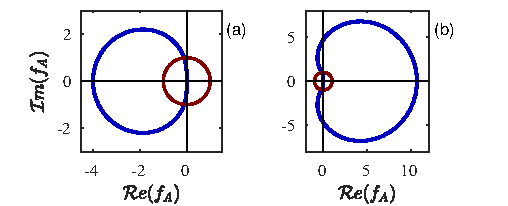
\includegraphics[width=0.95\columnwidth]{FacAmp.pdf}
\end{center}
\caption{(a) Facteur d'amplification $f_A$ du schéma décentré gauche à 3 points pour la dérivée première obtenu par analyse de Von-Neuman pour $a=1$ (bleu). Le cercle rouge représente le cercle unité. (b) Même chose pour le schéma décentré gauche à 5 points. Les courbes bleues restent dans le cercle rouge pour des modes de fréquence $|\theta| < \pi/4$ dans les deux cas, mais en dehors du cercle unité $f_A$ conserve une amplitude bien plus modérée dans le cas (a). Ainsi nous pouvons penser que dans notre schéma le schéma à 3 points à plus de chance d'être stable pour un même pas de discrétisation.}
\label{fig:FacAmp}
\end{figure}


\section{Resultats : Ising 2D}
\label{sec:ResIsing}
\subsection{Complexité algorithmique et parallélisation - problème de rapidité} 


Comme pour le modèle continu $\varphiv^4$ il est possible de paralléliser le code en utilisant de l'openMP \cite{openmp2002c++} grain fin sur les boucles en champ. En revanche, à cause de la quadrature précise que l'on a développé pour le calcul les intégrales $J$, le temps de calcul se trouve évoluer en $\mathcal{O}( Q_\text{max} \times n_c^3 \times n_{gl}^2 \times n_{\phi})$. Où $n_{\phi}$ est le nombre de point de discrétisation en champ, $n_c$ le nombre de points d'interpolation, $n_{{gl}}$ le nombre de points de la quadrature de Gauss-Legendre, et $Q_{\text{max}}$ est le rang maximal de l'approximation de rang faible de \refsec{Decomp2}. Pour le vérifier nous avons tracé les points de la \refig{timeNc}.


Ainsi nous pouvons constater l'évolution problématique du temps de calcul de cet algorithme de résolution. En revanche nous avons aussi étudié l'effet de la parallélisation sur les points de discrétisation en champ $\phi$. Pour un code pouvant être parallélisé au maximum sur 48 coeurs nous obtenons une décroissance en $\sim 1/n_{proc}$ où $n_{proc}$ est le nombre de processeur utilisé lorsque $n_{proc} \lesssim 30$. C'est donc au alentours de $30$ coeurs qu'il est préférable d'exécuter ce code. Le résultat est représenté en  \refig{timeScal}.


\begin{figure}[H]
\begin{center}
	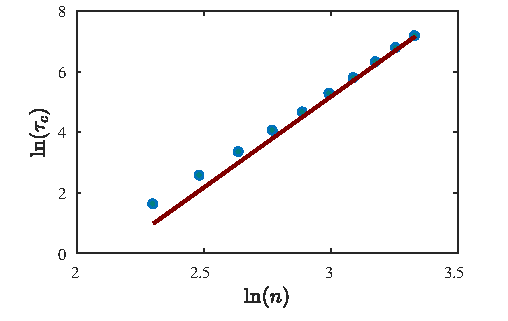
\includegraphics[width=0.95\columnwidth]{ComplexiteTemps.pdf}
\end{center}
\caption{(Points bleus) Logarithme du temps de calcul mesuré $\tau_c$ de 10 pas de temps du code en fonction du nombre de points d'intégration et d'interpolation, avec $n_\phi$ fixé. On a pris $n_c = n_{gl} = n$. (Ligne rouge) droite d'équation $y=6x+b$ avec $b$ une constante. Il semble que les points se rapproche du comportement de la droite et ainsi que l'on ait $t_c \propto n^6$. Un interpolation linéaire donne plus précisément $t_c \propto n^{5,7}$ pour les valeurs de $n$ représentées ici.}
\label{fig:timeNc}
\end{figure}



\begin{figure}[H]
\begin{center}
	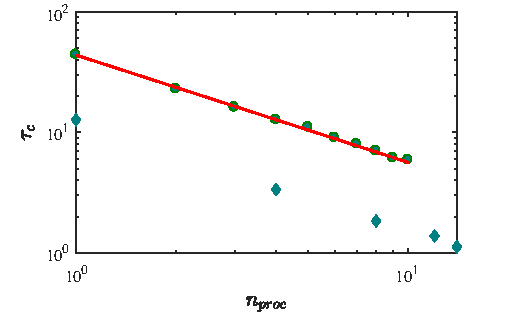
\includegraphics[width=0.95\columnwidth]{Scalabilite.pdf}
\end{center}
\caption{Évolution du temps de calcul $\tau_c$ d'un pas de temps de la résolution avec le nombre $n_{proc}$ de processeurs utilisés. Ce temps est déterminé en faisant une moyenne sur  plusieurs pas de temps de la résolution. (points verts) En exécutant le code sur les ordinateurs du laboratoires limités, pour ceux que nous avons pu utiliser, à 10 ou 12 cœurs. (losanges verts) En exécutant le code sur le calculateur Mesu. Les courbes continues rouges représentent la décroissance idéale en $1/n_{proc}$. Nous pouvons remarquer que sans même paralléliser sur un nombre de cœur plus important le calcul est plus rapide sur Mesu.}
\label{fig:timeScal}
\end{figure}


Le nombre de processeurs sur lesquels peut être parallélisé efficacement le programme est bridé par le nombre de points de la discrétisation en champ. Ainsi pour tenter d'augmenter la vitesse d'exécution nous avons réalisé une version du code avec une parallélisation MPI \cite{open2012open} de la boucle en champ et une parallélisation OpenMP des boucles de la quadrature de l'intégrale $J$, $\bJ$ ou $\tJ$. Il s'avère qu'alors il faut communiquer un nombre de données trop important entre les processeurs, le code s'en trouvait alors ralenti, voire inutilisable. \\







\subsection{Problème de précision des intégrales}


A cause de la complexité des algorithmes il n'est pas possible de choisi $n_c$ et $n_{gl}$ aussi grand qu'on le souhaite pour obtenir la precision voulue. Au début nous pensions qu'un nombre faible de points suffirait mais il s'avère que ce n'est pas spécialement le cas. En effet nous avons dû utiliser le calculateur Mesu \cite{ wiki:xxx} de l'université Pierre et Marie Curie pour pouvoir paralléliser notre programme sur un nombre de coeurs supérieur à $20$ et pouvoir augmenter $n_c$ et $n_{gl}$ sans dépasser les 72 heures permises pour une simulation sur la machine. Nous avons comparé les résultats obtenus pour différentes simulations en fixant $n_c = n_{gl} = n$. L'influence de $n$ est en \refig{etaErr}.

\begin{figure}[H]
\begin{center}
	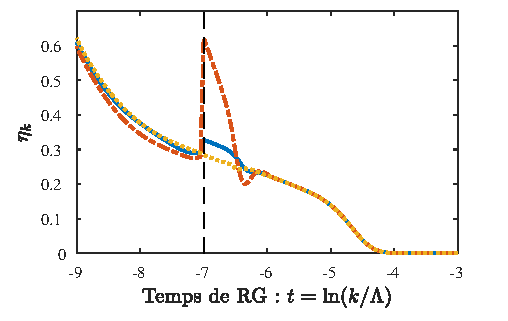
\includegraphics[width=0.95\columnwidth]{EtakErrMesu.pdf}
\end{center}
\caption{Évolution de $\eta_k$ en fonction de $t$ pour différentes valeurs du nombre de point d'interpolation et d'intégration (la courbe se lit de gauche à droite). (rouge discontinu) $n=14$, (bleu continu) $n=20$, (jaune pointillé) $n=22$. Le trait vertical noir se trouve à $t_b = \ln(k_b/\Lambda)$ correspondant au passage du problème ($\Pc_2$) au ($\Pc_3$). Avec une précision suffisante les courbes devraient être continues cependant ce n'est clairement pas le cas pour $n<22$. Même pour $n=22$ il y a une légère différence, mais surtout un épaulement proche de $t=-6$ que l'on ne saurait expliquer.}
\label{fig:etaErr}
\end{figure}

Ainsi pour $n=22$ les résultats semblent être relativement corrects avec toutefois quelques irrégularités. Ceci nous confirme qu'une partie des imprécisions sur les résultats que peut permettre de sortir ce code de simulation sont dues au calcul des intégrales. Malheureusement il n'est pas vraiment possible de quantifier cette erreur et de la comparer aux erreurs qui peuvent provenir aussi d'une discrétisation en champ pas assez précise ou d'un pas de temps trop élevé. \\



\subsection{Estimation de la température critique et de l'exposant critique $\eta$}

Enfin, malgré les erreurs que nous avons pu observer, provenant d'une précision non suffisante dans les calculs des intégrales nous avons tout de même tenté de récupérer la valeur de la température critique et de l'exposant $\eta$. Ainsi en utilisant $n_c = n_{gl} = 22$ nous avons obtenu une température critique dans l'encadrement

\begin{equation}
2.350 \, J/k_B < T_c^{BMW}  < 2.375 \, J/k_B
\end{equation}

Nous savons que la température critique théorique attendu est de $T_c^{th} = 2.2691 J/k_B$. Nous avons donc un résultat proche du résultat attendu avec une erreur 

\begin{equation}
	err = \frac{ |T_c^{BMW} - T_c^{th}|}{T_c^{th}} \sim 4 \%
\end{equation}


Comme nous pouvons le voir en \refig{etaMesu}, en plus de nous donner la température critique, le code nous permet aussi de retrouver $\eta$ autour de $0.25$ pour $d=2, N=1$ comme nous l'avions déjà déterminé en \refsec{ResContinu}.

\begin{figure}[H]
\begin{center}
	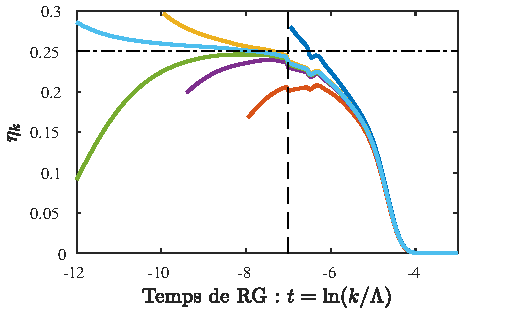
\includegraphics[width=0.95\columnwidth]{MesuRes.pdf}
\end{center}
\caption{Évolution de $\eta_k$ en fonction de $t$ pour différentes valeurs de la températue $T$ du système (la courbe se lit de droite à gauche). $n_c=22$, $n_{gl} = 22$. Le trait vertical noir se trouve à $t_b = \ln(k_b/\Lambda)$ correspondant au passage du problème ($\Pc_2$) au ($\Pc_3$). Le trait horizontal noir correspond à la valeur théorique $\eta = 0.25$ attendue. }
\label{fig:etaMesu}
\end{figure}

Les résultats sur la température critique $T_c$ dépendent de $\alpha$ et $\mu$ à cause de la discrétisation numérique. Ils dépendent aussi du nombre de point de discrétisation en champ utilisé. L'estimation précédente est donc une première estimation grossière que nous avons eu le temps de réaliser en prenant en compte ces variations, en revanche il serait nécessaire d'approfondir l'influence des différents paramètres pour obtenir une valeur plus précise et qui serait peut être plus proche de la valeur théorique attendue.


\section{Conclusion}

Les conclusions de cette étude se séparent en deux, celles pour le code de simulations du modèle continu $\varphiv^4$ et celles pour le code de simulation du modèle d'Ising. \\

Dans le premier cas nous avons réussi à réécrire le code pour le rendre plus modulable. En revanche même si l'on retrouve bien les bons résultats que ce code permettait déjà d'obtenir nous avons fait peu d'avancés sur la compréhension des instabilités qu'il présente. Nous avons fait varier de nombreux paramètres des discrétisations numériques sans avoir de résultats. Les seuls paramètres ayant une influence sont ceux relatif aux quadratures des intégrales numériques. C'est seulement en modifiant leur implémentation nous avons pu obtenir des exposants critiques proche de ce qui est attendu pour $d=2.1$, $N=2$. Cependant ces mêmes modifications du code peuvent donner des résultats moins bons pour d'autres paramètres $d$ et $N$ que ce qui avait déjà pu être obtenu par le code originel. Malheureusement nous n'avons pas eu le temps d'approfondir l'étude. \\


Pour ce qui concerne le code de simulation du modèle d'Ising 2D, en partant de zéro nous avons réalisé des simulations qui nous permettent de donner une estimation, éloignée d'environ $4 \%$ de la valeur théorique, de la température critique. Pour cela nous avons dû contourner de nombreux problèmes numériques en utilisant différentes méthodes. Cependant ces simulations présentent toujours des comportement étranges qui ne permettent pas d'avoir une totale confiance dans le résultat obtenu. L'étude mériterait d'être approfondie pour s'assurer qu'une résolution numérique d'équations BMW issues du NPRG permet d'obtenir avec une précision suffisante la température critique d'un système donné.

\vfill

\pagebreak

\bibliographystyle{plain}
\bibliography{Rapport}


\end{multicols}


\pagebreak

\appendix


\begin{multicols}{2}
\section{Outils pour le développement des équations}

\label{ann:outils}


\subsection{Notations des normes}

On définit les notations utilisée pour les normes. Soit $d \in \N^*$. Soit un vecteur  $\uv =(u_1, u_2, ... u_d) \in \R^d$, on définit
\begin{equation}
{\| \uv \|}_\infty =  \underset{i \in \bbrac{1,d}}{\text{max}}{|u_i|}\, ,
\end{equation} 
\begin{equation}
{\| \uv \|}_2 =  \sqrt{\sum_{i = 1}^{d} |u_i|^2} \, .
\end{equation}
Soit maintenant $\Omega \subset \R^d$. Soit $f \in \Cc^0(\Omega)$, on note
\begin{equation}
{\| f \|}_\infty =  \underset{x \in \Omega}{\text{sup}}{|f|} \, .
\end{equation} 


%Enfin, soit $N \in \N$ et $\fv$  $\in \(L^2(\Omega)\)^N$, 
%\begin{equation}
%{\| \fv \|}_2 = \sqrt{\sum_{i = 1}^{N} \left|\int_\Omega f_i(\rv) %\dd \rv \right|^2} \, .
%\end{equation} 

\subsection{Transformée de Fourier}

On rappelle ici les notations utilisée pour définir les transformées de Fourier. Pour cela on considère $\varphiv$ une application de $L^2(\R^d)^N$. On définit alors la transformée de Fourier de $\varphiv$, notée $\hat{\varphiv}$ ou $\text{TF}[\varphiv]$ par, 

\begin{equation}
  \forall \qv \in \R^d \quad \hat{\varphiv}(\qv) = \text{TF}[\varphiv](\qv) = \int_{\R^d} \varphiv(\rv) e^{-i\qv.\rv}\dd \,\rv
\end{equation}
Avec la relation inverse,
\begin{equation}
  \forall \rv \in \R^d \quad \varphiv(\rv)  = \text{TF}^{-1}[\hat{\varphiv}](\rv) = \frac{1}{(2\pi)^d}\int_{\R^d} \hat{\varphiv}(\qv) e^{i\qv.\rv}\dd \,\qv
\end{equation}
On utilise alors la notation plus compacte 
\begin{equation}
  \frac{1}{(2\pi)^d}\int_{\R^d} ... \dd \,\qv \equiv \int_\qv ... \quad \text{et} \quad  \int_{\R^d} ... \dd \,\rv \equiv \int_\rv ... 
\end{equation}

Dans le cas ou l'on a des fonctions définies non pas sur $\R^d$ mais sur un domaine $\Omega \subset \R^d$ fini alors nous aurons les mêmes propriétés avec la relation "d'équivalence"  
\begin{equation}
	 \int_{\qv} ... \overset{\text{$\Omega$ fini}}{\quad \longrightarrow \quad } \frac{1}{\Omega} \sum_{\qv} ...
\end{equation}
Remarquons que lorsque l'on introduit la transformée de Fourier (\refsec{}) pour l'utiliser dans le RG les fonctions $\varphiv$ sont tout d'abord définies sur un ouvert $\Omega$ fini mais par des considérations physique, en passant à "la limite thermodynamique" on en vient à considèrer $\Omega$ comme devenant $\R$ tout entier. En outre, dans le cas où $\varphiv \in \Sr'(\R^d)^N$ (espace des distributions tempérées) on étend la notion de transformée de Fourier $\hat{\varphiv}$ de $\varphiv$ à l'aide du crochet de dualité, 
\begin{equation}
  \forall u \in \Sr(\R^d, \R^N) \quad \left< \hat{\varphiv}, u \right>_{\Sr', \Sr} = \left< \varphiv, \hat{u} \right>_{\Sr', \Sr}
\end{equation}

\vspace*{11pt}



\subsection{Transformée de Fourier Semi-Discrète (TFSD)}

\label{ann:TFSD}

Dans le modèle d'Ising à deux dimensions nous introduisons une transformée de Fourier semi discrète car nous travaillons non pas avec des fonctions mais avec des suites. Ainsi soit $\varphi_\rv \in \ell^2$. On peut définir $\hat{\varphi} \in L^2(\R)$ par  
\begin{equation}
  \hat{\varphi}(\qv) = \sum_\rv \varphi_\rv e^{-i\qv\rv}
\end{equation}
  Avec la relation inverse,
\begin{equation}
 \varphi_\rv = \int_{\R^d} \hat{\varphi}(\qv)  e^{i\qv\rv} \dd\, \qv \equiv \int_\qv \hat{\varphi}(\qv)  e^{i\qv\rv}
\end{equation}
On peut de plus démontrer que cette transformation est une isométrie \cite{}.



\vspace*{11pt}
\subsection{Derivation fonctionnelle}

\subsubsection{Définition}
Soit $U$ et $V$ deux espaces de Banach. Soit $F$ une fonctionnelle de $U$ dans $V$. 
Soit $f \in U$. On appelle, si elle existe, dérivée (au sens de Fréchet) de la fonctionelle $F$ prise en $f$, l'application linéaire continu de $\mathcal{L}(U,V)$, notée $D_fF$ telle que, pour $\eps>0$, 
\begin{equation}
\forall h \in U \quad \lim_{ \eps \rightarrow 0 } \frac{\| F[f+\eps h] - F[f] - \eps D_fF.h\|_V}{\eps}  = 0
\end{equation} 
Dans le cas où $U = L^2(\R^d)^N$ et $V = \R$ alors $D_fF \in U'$ (espace des forme linéaires continues de $U$) et on sait qu'il existe, par le théorème de Frechet-Riesz, une quantité unique que l'on note $\delta F[f]/\delta f \in U'(\simeq U)$ telle que 
\begin{equation}
\forall h \in U \quad D_f F.h = {\left< \derd{F[f]}{f}, h \right>}_{U} = \int \derd{F[f]}{f(\rv)} h(\rv) \dd \, \rv	
\end{equation}

\vspace*{11pt}

\subsubsection{Transformée de Fourier d'une dérivée fonctionnelle}

Soit $F$ une fonctionelle de $U = L^2(\R^d)^N$ dans $(\R,|.|)$ et $\varphiv \in U$.
Soit $\rv \in \R^d$.
Alors, 
\begin{equation}
  \derd{F}{\varphiv(\rv)} = \int_{\qv} \derd{F}{\hat{\varphiv}(-\qv)} e^{i\qv.\rv} = \text{TF}^{-1} \left[ \derd{F}{\hat{\varphiv}(-\qv)} \right](\rv) 
\end{equation} 
Et réciproquement nous avons alors aussi, pour $\pv \in \R^d$,  
\begin{equation}
  \derd{F}{\hat{\varphiv}(-\pv)} = \int_{\rv} \derd{F}{\varphiv(\rv)} e^{-i\pv.\rv} = \text{TF} \left[ \derd{F}{\varphiv(\rv)} \right](\pv) 
\end{equation} 

\vspace*{11pt}
%\noindent
{\footnotesize 
\noindent
En effet, par la règle de la chaine de la dérivation de Fréchet nous pouvons écrire, 
\begin{equation}
  \forall \hv \in U \quad D_{\varphiv} F. \hv = D_{\hat{\varphiv}} F. D_{\varphiv} \hat{\varphiv}.\hv 
\end{equation}
Cependant, $\hat{\varphiv}$ est une fonctionnelle de $\varphiv$ (par définition de la TF) de $U$ dans $U$ qui est linéaire en $\varphiv$. Soit $\eps >0$, 
\begin{equation}
  \forall \hv \in U \quad \hat{\varphiv}[\varphiv + \eps \hv] - \hat{\varphiv}[\varphiv] = \eps \hat{\hv} 
\end{equation} 
Il vient directement, par définition de la dérivation au sens de Frechet, $D_{\varphiv} \hat{\varphiv} .\hv = \hat{\hv}$.  
Ainsi,  $D_{\varphiv} F .\hv = D_{\hat{\varphiv}}F.\hat{\hv}$.  On peut alors écrire, 
\begin{align}
  \forall \hv \in U  \quad D_{\varphiv} F .\hv & = \int_{\qv} \derd{F}{\varphiv(\qv)} \int_{\rv} \hv(\rv) e^{-i\qv.\rv} \\
  \forall \hv \in U  \quad D_{\varphiv} F .\hv & = \int_{\rv} \int_{\qv} \derd{F}{\varphiv(\qv)} e^{-i\qv.\rv } \hv(\rv)
\end{align}
}



\subsection{Opérateurs à noyaux}

Nous détaillons dans cette sections quelques propriétés élémentaires des opérateurs à noyaux. Pour plus de détails on pourra regarder \cite{}. Ceci permet de comprendre quelques unes des étapes dans la détermination des équations de flot et BMW. \\



\subsubsection{Définition}

On appelle $S$ un operateur a noyaux, une application de $(L^2(\R^d))^N$, telle que pour tout $(i,j) \in \bbrac{1,N}^2$, il existe une application $A_{i,j} \in L^2(\R^d\times\R^d)$ telle que,  pour tout $\varphiv \in (L^2(\R^d)^N$ et $\rv \in \R^d$
 \begin{equation}
  S[\varphiv]_i(\rv) = \int_{\rv'} \sum_{j=1}^{N} A_{i,j}(\rv,\rv')\varphi_j(\rv')
 \end{equation}
 La matrice $A : (\rv,\rv') \rightarrow ((A_{i,j}(\rv,\rv')))_{i,j}$ est appelée noyau de $S$.  On identifiera alors dans les notations $S$ et $A$ indépendamment. Par Cauchy-Schwartz cette définition a bien  un sens. De plus, on peut montrer que $S$ et est un endomorphisme de $(L^2(\R^d)^N$. Pour plus de clarté, nous utiliserons par la suite la notation d'Einstein : on n'écrit plus la somme sur $j$ dans l'expression de $S$, et de manière générale lorsque un indice est répété dans une expression on suppose qu'il est sommé de $1$ à $N$, 
  \begin{equation}
  S[\varphiv]_i(\rv) \equiv \int_{\rv'} A_{i,j}(\rv,\rv')\varphi_j(\rv')
 \end{equation}
 



\vspace*{11pt}

\subsubsection{TF d'un opérateur à noyau}

Nous avons vu que $S$ définie comme précédemment était un endomorphisme de $(L^2(\R^d)^N$. Ainsi il est possible d'en définir la transformée de Fourier. Introduisons tout d'abord la transformée de Fourier du noyaux, pour $(i,j) \in \bbrac{1,N}^2$ et $(\qv, \qv') \in (\R^d)^2 $
\begin{equation}
	 \hat{A}_{i,j}(\qv, -\qv') = \iint_{\rv,\rv'} A_{i,j}(\rv,\rv')\,e^{-i\qv.\rv} \, e^{-i \qv'.\rv'} 
\end{equation}
Ce qui implique alors 
\begin{equation}
	 \hat{S}[\varphiv]_i(\qv) = \int_{\qv'} \hat{A}_{i,j}(\qv, -\qv') \hat{\varphi}_j(\qv')
\end{equation}



{\footnotesize
\noindent
En effet, ceci ce démontre en développant le calcul de la transformée de Fourier. Soit $\qv \in \R^d$, $i \in \bbrac{1,N}$
\begin{align}
 \hat{S}[\varphiv]_i(\qv)  = & \int_{\rv} \int_{\rv'} A_{i,j}(\rv,\rv')\varphi_j(\rv') e^{-i\qv\rv}  \\
\hat{S}[\varphiv]_i(\qv)  = & \iint_{\rv, \rv'} \int_{\qv'} A_{i,j}(\rv,\rv') \hat{\varphi}_j(\qv') e^{i\qv'\rv'} e^{- i\qv\rv} \\
 \hat{S}[\varphiv]_i(\qv)  = &   \int_{\qv'} \hat{\varphi}_j(\qv') \left\{ \iint_{\rv, \rv'} A_{i,j}(\rv,\rv')  e^{i\qv'\rv'} e^{- i\qv\rv}  \right\}  \\
\hat{S}[\varphiv]_i(\qv) = & \int_{\qv}  \hat{\varphi}_j(\qv') \hat{A}_{i,j}(\qv, -\qv')
\end{align}
}

\vspace*{11pt}

\subsubsection{Composition de deux opérateurs}

Considérons deux opérateurs à noyaux, $S$ et $T$ de noyaux respectifs $A$ et $B$. La composition de ces deux opérateurs est définie, pour $\rv \in \R^d$, par
\begin{equation}
 	S . T [\varphiv]_i (\rv) = \int_{\rv'}  \left\{ \int_{\rv''} A_{i,k}(\rv, \rv'')B_{k,j}(\rv'', \rv') \right\} \varphi_j(\rv')
\end{equation}
On notera alors aussi pour $(\rv, \rv') \in (\R^d)^2 $
\begin{equation}
   (A . B)_{i,j} (\rv, \rv') = \int_{\rv''} A_{i,k}(\rv, \rv'')B_{k,j}(\rv,'' \rv') 
\end{equation}
Par transformée de Fourier, et par un calcul analogue à celui fait pour un simple noyau, il vient, pour $(\qv, \qv') \in (\R^d)^2$,
\begin{equation}
	\widehat{(A . B)}_{i,j}(\qv, \qv') =\int_{\qv''} \hat{A}_{i,k}(\qv, \qv'')\hat{B}_{k,j}(-\qv'', \qv') 
\end{equation}



\vspace*{11pt}

\subsubsection{Trace d'un opérateur à noyau}

On définit la trace d'un opérateur $S$ de noyaux $A$ par
\begin{equation}
  \text{Tr}\, S \equiv \text{Tr} \, A = \int_{\rv} A_{i,i}(\rv,\rv) 
\end{equation}
Nous pouvons alors de manière similaire à ce qui a été fait pour démontrer l'expression de la transformée de Fourier d'un opérateur à noyau, calculer la relation sur la trace de la transformée de Fourier
\begin{equation}
  \text{Tr} \hat{A} =  \int_{\qv} \hat{A}_{i,i}(\qv,-\qv) 
 \end{equation}



\vspace*{11pt}



\subsubsection{Inverse d'un opérateur à noyau}

Soit S un opérateur à noyau de noyaux A. On fait l'hypothèse, sans justifications, que pour les systèmes physiques que l'on étudie il existe une grandeur appelée l'inverse de S, également un opérateur à noyau, endomorphisme de $(L^2(R^d))^N$, notée $S^{-1}$ telle que, pour $i \in \bbrac{1,N}$ et $\varphiv \in (L^2(R^d))^N$, 
\begin{equation}
	\forall \rv \in \R^d \quad S.S^{-1}[\varphiv]_i(\rv) = \varphi_i (\rv)	
\end{equation}

Si $A$ est le noyau de $S$, on note $A^{-1}$ le noyau de $S^{-1}$. \\



\pagebreak


\section{Compléments théoriques}
\subsection{Détails du formalisme du RG}


Nous détaillons ci-après le formalisme du RG pour parvenir à calculer la fonction de partition de systèmes décrits avec des champs. Cette présentation reprend le texte principal mais va plus loin dans les explications.



Les principales idées du RG ont été développées par Wilson \cite{wilson1971renormalization, wilson1971renormalization2,fisher1998renormalization}. L'objectif est de calculer la fonction de partition à champ magnétique extérieur $\bv$ nul,
\begin{equation}
	\Zc[T] = \int \Dc \varphiv \, \exp\(- H[\varphiv] \) \, . 
\end{equation}
L'idée du RG est de ne pas considérer tous les degrés de liberté dans l'expression de $\Zc$ sur le même pied d'égalité. En effet, on commence d'abord, pour calculer $\Zc$, par intégrer les degrés de libertés de grand moment $\pv$ entre $k = \Lambda/s$ et $\Lambda$ où $k \in [0,\Lambda]$. En pratique cela signifie que l'on sépare $\varphiv$ en deux fonctions $\varphiv_>$ et $\varphiv_<$ telles que $\varphiv(\pv) = \varphiv_{k,>}(\pv) + \varphiv_{k,<}(\pv)$ et
\begin{align}
	\varphiv_{k,>}(\pv)  = 
\begin{cases}
\quad \varphiv(\pv) \quad & \text{si} \quad \pv \in   [k,\Lambda] \\
 \quad 0 \quad & \text{sinon}
\end{cases}
\end{align}
Ceci permet de définir un hamiltonien effective $H_k$, 
\begin{equation}
	H_k[\varphiv_{k,<}] \equiv \int \Dc \varphiv_{k,<}  \exp \{ H[\varphiv_{k,>}+ \varphiv_{k,<}] \},
\end{equation}
(on oublie la dépendance en $\bv$ dans la notation), 
et de réécrire la fonction de partition comme 

\begin{equation}
\Zc = \int \Dc \varphiv_{k,<} \, \exp\left\{- H_k[\varphiv_{k,<}]\right\}. 
\end{equation} 

De manière générale l'hamiltonien $H$ ne s'exprime pas seulement en fonction du champ $\varphiv$ mais son expression contient aussi des constantes de couplage qui caractérisent la physiqu du système. Dans le modèle d'Ising 2D, $J$ est une constante de couplage par exemple.  Ces constantes sont notées $\{g_i\}_i$ avec $i \in \N$. On écrit alors $H[\varphiv] = H[\varphiv ; \{g_i\}]$. Le nouvel hamiltonien $H_k[\varphiv_{k,<}]$ peut alors s'exprimer aussi sous la forme $H_k[\varphiv_{k,<} ; \{g_{k,i}\}_i]$ où $\{g_{k,i}\}_i$ sont de nouvelles constantes de couplage. \\

Bien entendu, il n'est pas directement possible de calculer $H_k$ pour $k$ quelconque, sinon le problème serait résolu en calculant $\Sc_0$. On considère alors plutôt une intégration infinitésimale entre $[\Lambda - d\Lambda, \Lambda]$ pour obtenir le nouvel hamiltonien $H_{k_1}$, où $k_1 = \Lambda - d\Lambda$. On introduit aussi $s_1 = \Lambda/k_1$. Ce calcul là, contrairement au calcul direct pour $k$ quelconque, peut être réalisé grâce à des approximations comme nous le détaillerons ensuite. Maintenant, avec l'expression de ce nouvel hamiltonien, on réalise ce que l'on appelle un adimensionnement qui se déroule en trois étapes listées ci-dessous.

 Tout d'abord, comme $\pv$ est homogène à $\text{L}^{-1}$ (ou L est la dimension d'une longueur) on introduit $\tilde{\pv} = s_1 \pv$. Ensuite on montre que le champ $\varphiv_{k_1, <}$ est homogène à $\text{L}^{d-2-\eta}$ (avec $\eta$ l'exposant critique défini dans l'introduction), on pose donc $\tilde{\varphiv}_{k_1, <}$ tel que $\varphiv_{k_1, <}(\pv) = s_1^{-d+2+\eta} \tilde{\varphiv}_{k_1, <}(\tpv)$ pour tout $\pv \in [0, \Lambda]^d$. Enfin la constante $g_{k_1, i}$ pour tout $i\in \N$ est aussi homogène à $\text{L}^{b_i}$ avec $b_i$ une constante. On écrit donc de nouvelles constantes de couplage $\{\tilde{g}_{k_1, i}\}_i$ telles que $g_{k_1, i} = s_1^{-b_i} \tilde{g}_{k_1, i}$. Ceci définit un hamiltonien $\tilde{H}$,
 \begin{equation}
 	\tilde{H}_{k_1}[\tilde{\varphiv}_{k_1,<}; \{\tilde{g}_{k_1, i}\}_i ] = H_{k_1}[\varphiv_{k_1,<}; \{g_{k_1,i}\}_i]
 \end{equation}
La fonction de partition (dont il ne sert en fait à rien de connaitre le préfacteur numérique) est alors simplement exprimée comme 
\begin{equation}
\Zc \propto \int \Dc \tilde{\varphiv}_{k_1,<} \, \exp\left\{- \tilde{H}_{k_1}[\tilde{\varphiv}_{k_1,<}, \{\tilde{g}_{k_1, i}\}_i ] \right\}. 
\end{equation} 


Ce changement est purement technique cependant il a un fondement physique puisqu'il permet de faire comme si $\tilde{H}_{k_1}$ était l'hamiltonien d'un "nouveau système" identique au système originel étudié mais dans lequel toutes les échelles de moment ont été dilatées d'un facteur $s_1$ et les échelles de longueur alors réduites d'un facteur $s_1$. Or on rappelle que pour une transition de phase du second ordre la longueur $\xi$ du système originel diverge pour $T \to T_c$. Ce "nouveau système" possède alors une longueur de corrélation $\xi_1 = \xi/s_1$ qui diverge aussi à la transition : $\xi, \xi_1 \to \infty$. Ainsi, à la transition de phase, et uniquement à la transition, les deux systèmes possèdent la même physique. Si $\xi$ ne divergeait pas (et donc si l'on n'était pas à la transition de phase) ce ne serait pas le cas puisque alors $\xi_1 \neq \xi$, et deux systèmes avec des longueurs de correléations différentes, ne représenteraient pas la même chose. \\

 Pour réaliser l'intégration complète sur $[0, \Lambda]$ on peut donc ensuite itérer ce processus de transformations infinitésimales en repartant de l'expression de $\Zc$ en fonction de $\tilde{H}_{k_1}[\tilde{\varphiv}_{k_1,<}, \{\tilde{g}_{k_1, i}\}_i ]$. On reproduit le même procédé, par exemple au deuxième pas de l'itération, en calculant l'intégration infinitésimale entre $[\Lambda - 2d\Lambda, \Lambda - d\Lambda]$ avec $k_2 = \Lambda - 2d\Lambda$. A la fin de cette deuxième itération nous avons donc intégré sur $[\Lambda - 2d\Lambda, \Lambda]$.  \\
 
 
 
On introduit à l'itération $p \in \N$ - itération à laquelle on a intégré sur $[k_p, \Lambda]$ - l'opérateur $O_p$ qui envoie $\{\tilde{g}_i\}_i$ sur $\{\tilde{g}_{k_p,i}\}_i$. L'hypothèse fondamentale du RG, qui n'est pas prouvée mais toujours vérifiée, est qu'il existe un point fixe de $O_p$ pour $p \to \infty$, si l'on est à la température critique (et/ou pression critique, ...). Ceci signifie plus exactement qu'il existe $\{\tilde{g}^*_i\}_i$ tel que 
 \begin{equation}
 	\lim\limits_{k \rightarrow \infty}  \tilde{g}_{k,i} = \lim\limits_{\substack{p \to \infty \\ d\Lambda \to 0 }}  \tilde{g}_{k_p,i} =  \tilde{g}^*_i
 \end{equation} 
Sans entrer plus en profondeur dans les calculs du RG on admet que l'on peut montrer que l'existence de ce point fixe explique l'universalité des exposants critiques \cite{Delamotte2012}. Deux systèmes avec les mêmes propriétés de symétries auront le même point fixe, ce qui revient à dire d'une autre manière qu'ils auront bien un comportement, une physique, identique à la transition de phase, quand la longueur de corrélation est infinie. \\
 
Dans un calcul de RG on prend classiquement un nombre fini de constantes de couplage et on considère qu'elles sont suffisamment faibles pour faire des développements du hamiltonien en puissances de ces constantes adimensionnées à chaque itération. Ce sont ces approximations qui permettent de faire des calcul mais elles limitent les applications possibles. Le NPRG développe alors une technique reprenant la même idée de calcul mais sans faire ces approximations, grâce à une astuce.

\vspace*{11pt}




\subsection{Fonctions de corrélation dans le calcul du NPRG}
\label{ann:FuncCorrel}

Dans le formalisme du NPRG il est possible de définir un tenseur de fonctions de corrélations connectées à deux points\footnote{Notons qu'il est très facile d'extrapoler la définition suivante à un tenseur de fonctions de corrélations connectées à $n \in \N$ points}. Pour cela on introduit l'énergie libre effective du système
\begin{equation}
W_k[\bv]	= \ln(\Zc[\bv])
\end{equation}
On considère ensuite $\rv_1$ et $\rv_2$ deux positions. On définit $i_1 \in \bbrac{1,N}$ un indice représentant un degré de liberté à la position $\rv_1$. De même on définit aussi $i_2$ représentant une degré de liberté à la position $\rv_2$,
\begin{equation}
  G^{(2)}_{c, k, i_1 i_2} [\rv_1, \rv_2 ; \bv] \equiv \derd{^2 W_k[\bv]}{b_{i_1}(\rv_1)\delta b_{i_2}(\rv_2)} \, .
\end{equation}
En transformée de Fourier elle devient
\begin{equation}
  G^{(2)}_{c, k, i_1 i_2} [\pv_1, \pv_2 ; \bv] \equiv \derd{^2 W_k[\bv]}{b_{i_1}(-\pv_1)\delta b_{i_2}(-\pv_2)}
\end{equation}
Cette fonction de corrélations ressemble fortement celle à deux points que nous avions introduite pour le modèle d'Ising 2D à la subtilité que l'on utilise $W$ et non pas $\Zc$ dans le numérateur. On comprendra donc qu'elle contiennent aussi l'information sur les exposants critiques $\eta$ et $\nu$. On s'intéresse plus particulièrement à l'expression de $G^{(2)}_{c,k,ii}$ pour $i \in \bbrac{1,N}$ pris en $\{\pv, -\pv\}$. En effet seul ce cas là a une utilité dans les équations de flot. On notera donc cette expression, pour être concis,
\begin{equation}
	G_{k,ii}[\pv; \hv] \equiv   G^{(2)}_{c,k, i i}[\pv, -\pv; \hv] = \derd{^2 W_k[\hv]}{b_{i}(-\pv)\delta b_{i}(\pv)} \, .
\end{equation}
On montre alors qu'au sens d'inverse des opérateurs
\begin{equation}
  G_{k}[\pv ; \hv] = \(\Gamma^{(2)}_{k}[\pv, \phiv] + \Rc_k(\pv)\)^{-1} 
\end{equation}


\vspace*{11pt}



\subsection{Ecriture du système d'équations BMW pour $\mathbb{Z}_2$} 

\label{ann:BMWON}

Tout d'abord, la condition initiale \refeq{initBMW} devient ici,
\begin{equation}
	\Gamma^{(2)}_\Lambda(\pv, \phi) = \pv^2 + r_0 + \frac{u_0}{2} \phi^2 \, .
	\label{eq:initBMWCont}
\end{equation}
On introduit aussi le potentiel du système, qui s'exprime simplement par,   
\begin{equation}
	V_k(\phi) = \Gamma_k(\pv, \phi) \, .
\end{equation}
Il vient alors\footnote{Dans les notations on note de la même manière une fonction de $\rho$ et une fonction de $\phi$, on écrit par exemple $V_k(\rho = \phi^2/2) = V_k(\phi)$.} en dérivant
\begin{equation}
	\Gamma^{(2)}_k(p=0, \rho) = \partial_{\rho}V_k(\rho) + 2\rho\partial_{\rho}^2 V_k(\rho) = \partial_{\phi}^2 V_k(\phi)
\end{equation}
En particulier il est plus précis d'utiliser en complément de l'équation sur $\Gamma^{(2)}_k$ l'équation de flot BMW que l'on peut aussi écrire sur $V_k$. Pour cela on introduit une fonction $\Delta_k(p, \rho)$ vérifiant la relation
\begin{equation}
	\Gamma^{(2)}_k(p, \rho) = p^2 + \Delta_k(p, \rho) + \partial_{\rho}V_k(\rho) + 2\rho\partial_{\rho}^2 V_k(\rho) \, .
	\label{eq:gammaDecomp}
\end{equation}
L'équation de flot BMW \refeq{flotBMW} peut alors se réécrire sous la forme du système couplé
\begin{align}
	\partial_t \Delta_k(p, \rho) & = 
	\begin{aligned}[t]
	 & 2\rho J_3(p,\rho){\left[u_k(\rho) + \partial_\rho \Delta_k (p,\rho) \right]}^{2} \\
	  & \, - \frac{1}{2}I_2(\rho) \left[\partial_\rho \Delta_k(p, \rho) +  2\rho \partial_\rho^2 \Delta_k(p,\rho) \right] \\
	 & \, - 2\rho I_3 (\rho) u_k^2(\rho) 
	 \end{aligned}
	\label{eqn:sysDeltaON1}\\
	\partial_t V_k(\rho) & = 
	\begin{aligned}[t]
		& I_1(\rho)
	\end{aligned}
	\label{eqn:sysDeltaON2}
\end{align}

Avec les notations
\begin{equation}
 \begin{split}
	m_k^2(\rho) & = 2\rho \partial_\rho^2 V_k(\rho) + \partial_\rho V_k(\rho)  \\
	u_k(\rho)  & = \partial_\rho m^2_k(\rho) \, 
	\end{split}	
\end{equation}
et toujours avec $\partial_t ... = k \partial_k ... $. La condition initiale se déduit de \refeq{initBMWCont}. En effet, il vient directement par la décomposition \refeq{gammaDecomp},
\begin{equation}
\Delta_\Lambda (p,\rho) = 0 \quad \text{et} \quad V_\Lambda(\rho) = r_0\rho + \frac{u_0}{6}\rho^2 \, .
\end{equation}

Maintenant que l'on a décomposé l'équation en système pour plus de précision nous allons plutôt travaillé avec la dérivée $W_k$ du potentiel pour des raisons de stabilité numérique, on note 
\begin{equation}
	W_k(\rho) = \partial_\rho V_k(\rho) \, .
\end{equation}

Il reste alors une dernière étape avant de parvenir aux équations finales. En effet, nous n'avons pas ici réalisé l'adimensionnement fondamental du RG. Pour cela il suffit d'introduire de nouvelles grandeurs notées d'un $\tilde{.}$ de la même manière qu'en \refsec{RG}. Concrètement cela revient à introduire, en utilisant le $Z_k$ défini en \refsec{DimAnorm}, 
\begin{equation}
\begin{split}
	& \trho  = k^{2-d}Z_k\rho \quad \text{et} \quad \tp = k^{-1}p\\
	& \tilde{m}^2_k(\rho) = Z_k^{-1} k^{-2} m^2_k(\rho), \\  
	& \tilde{u}_k(\trho) = Z_k^{-2}k^{d-4}u_k(\rho) \\
	& \tG_k(\tp,\trho) = Z_k k^2 G_k(p,\rho) \\
	& \tJ_n(\tp, \trho) = Z_k^{n-1} k^{2n -d-2}J_n(p,\rho) \\
	& \tV_k(\trho) = k^{-d} V_k(\rho)
	\end{split}
\end{equation}
Ainsi que
\begin{equation}
	\tY_k(\tp, \trho) = \frac{1}{Z_k}\( 1+ \frac{\Delta_k(p,\rho)}{p^2}\)-1 \, .
\end{equation}

Ce changement de variable en plus d'être nécessaire pour trouver le point fixe apporte de grands changements dans la forme des équations. En effet, on multiplie les expressions et les variables par des facteurs contenant $k$ ou $Z_k$ qui possèdent des dérivées non nulles lorsque l'on leur applique l'opérateur différentiel $\partial_t$. La nouvelle forme du problème que nous avons essayé de résoudre numériquement est :\\

\noindent
{\itshape Trouver $\tY_k(\tp, \trho)$ et $\tW_k(\trho)$ tels que pour tout $k \in ]0 ,\Lambda]$,  $\trho \in [0, +\infty[$ et $\tp \in [0, +\infty[$,}
\begin{align}
	\partial_t \tY_k & = 
	\begin{aligned}[t]
			& \eta_k(1+\tY_k) + \tp \, \partial_{\tp} \tY_k -(2-d-\eta_k)\trho \,\partial_{\trho} \tY_k  \quad  \\
			& \quad + 2\trho \tp^{-2} \left[ {\( \tp^2 \partial_{\trho} \tY_k + \tilde{u}_k\)}^2\, \tJ_3 - \tilde{u}_k^2\ \tI_3 \right] \\
			& \quad - \tI_2 \(  \partial_{\trho} \tY_k / 2 + \trho \,  \partial_{\trho}^2 \tY_k \)
	\end{aligned}
	\label{eqn}\\
	\partial_t \tW_k & = 
	\begin{aligned}[t]
		& (\eta_k-2) \tW_k  + (d-2+\eta_k) \trho \,\partial_{\trho}\tW_k + \frac{1}{2} \partial_{\trho} \tI_1
	\end{aligned}
\end{align}
\textit{Avec les conditions initiales,}
\begin{equation}
	\tY_\Lambda(\tp, \trho) = 0 \quad  \text{et} \quad \tW_\Lambda(\trho) = r_0' + u_0'\trho
\end{equation}
où $r_0'$ et $u_0'$ viennent de $r_0$ et $u_0$ (c.f. \refeq{hamiltCont}). 
Pour résoudre ce système il manque encore l'expression de $\eta_k$ pour $k$ fixé, découlant de la définition même de $Z_k$ en \refeq{defZk} (en choisissant $\phiv_0 = 0$ et $\pv_0 = 0$),
\begin{equation}
\eta_k = \frac{1}{2}  \tI_2(\rho = 0)\partial_\rho\tY_k(\rho = 0) \, .
\end{equation}

\vspace*{11pt}





\subsection{Modélisation du modèle d'Ising 2D avec des champs}


\label{ann:IsingChamp}

Nous détaillons ici le calcul permettant d'écrire l'hamiltonien d'Ising 2D comme un hamiltonien dépendant de champs. Commençons alors la transformation pour obtenir une fonction de partition s'exprimant avec des champs et décrivant le modèle d'Ising 2D. Afin d'écarter un problème qui apparaitrait dans la suite des calculs nous commençons par définir un hamiltonien du modèle d'Ising légèrement modifié. Pour $\Mr$ micro-état, on pose 
\begin{align}
  H_\mu(\Mr) &= -J \sum_{\left<\rv, \rv'\right>}S_\rv S_{\rv'} - \mu N_S \\
  H_\mu(\Mr)   &= -J\sum_{\left<\rv, \rv'\right>}S_\rv S_{\rv'} - \mu \sum_\rv S_\rv^2 
\end{align}
Avec les notations du modèle d'Ising, $L+1$ étant le nombre de spins dans une direction, la somme sur $\rv$ signifie
\begin{equation}
\sum_\rv \,\, ... \equiv \sum_{m=0}^{L}\sum_{n=0}^{L} \, ... \, ,
\end{equation}
où $\rv \equiv m\ev_x + m\ev_y$. La pas $a$ du réseau n'apparait pas car, pour simplifier les calculs, on exprime ici toutes les longueurs en unité du pas du réseau. Le nombre $N_s \equiv (L+1)^2$ est le nombre total de spins. Physiquement, ajouter une constante à $H$ ne change rien car cela ne fait que décaler l'origine arbitraire des énergies. En revanche cela a un avantage mathématique. En effet, on pose $A_{\rv, \rv'}^{(\mu)}$ la matrice définie implicitement dans $\mathcal{M}_{L+1, L+1}(\R)$ (espace des matrices réelles carrés $L+1$ par $L+1$) par
\begin{equation}
  H_\mu  = -\frac{1}{2} \sum_{\rv, \rv'} S_\rv A_{\rv, \rv'}^{(\mu)}S_{\rv'}
\end{equation}

Il est alors possible de choisir $\mu$ suffisamment grand pour que $A_{\rv, \rv'}^{(\mu)}$ soit à diagonale strictement dominante et donc inversible. Il suffit de prendre $\mu > 2J$. Cette condition d'inversibilité sera primordiale pour pouvoir aboutir à un résultat.\\


Maintenant que cette première étape a été réalisée on peut réaliser la transformée de Hubbard-Stratanovitch nous permettant d'écrire la fonction de partition du système avec des variables définies dans $\R$. Pour cela commençons par écrire la fonction de partition du système modèle (en intégrant le terme $(1/k_BT)$ dans $H_\mu$), 
\begin{equation}
  \Zc = \sum_{\Mr} e^{-H_{\mu}(\Mr)} =\sum_{\Mr}  \exp\(-\frac{1}{2} \sum_{\rv, \rv'} S_\rv A_{\rv, \rv'}^{(\mu)}S_{\rv'}\) \, .
\end{equation}
La transformée de Hubbard-Stratanovitch est, en fait, une simple integration gaussienne \textit{inverse}, il vient, 
\begin{equation}
\begin{split}
  \Zc & \propto \sum_{\Mr} \int_\R \prod_{\rv} \, \dd \varphi_\rv \, e^{ -\frac{1}{2} \sum\limits_{\rv, \rv'} \varphi_\rv {(A_{\rv, \rv'}^{(\mu)})}^{-1} \varphi_{\rv'} +\sum\limits_\rv  \varphi_\rv S_\rv  } \\
  \Zc & \propto \int_\R \prod_{\rv} \, \dd \varphi_\rv \, e^{ -\frac{1}{2} \sum\limits_{\rv, \rv'} \varphi_\rv {(A_{\rv, \rv'}^{(\mu)})}^{-1} \varphi_{\rv'} + \sum\limits_\rv \ln\(\cosh(\varphi_\rv)\) } \,. 
\end{split}
\end{equation}

Les variables $\varphi_\rv$ sont à valeur dans $\R$ tout entier. Cependant cela soulève un autre problème. En effet nous ne pouvons pas exprimer facilement ${(A_{\rv, \rv'}^{(\mu)})}^{-1}$ (qui existe bien car $A_{\rv, \rv'}^{(\mu)}$ est inversible). Pour cela il est pratique de réaliser une transformée de Fourier Semi-Discrète (TFSD - c.f. \refann{TFSD}) en posant, pour $\qv \in [-\pi, \pi]^2$,
\begin{equation}
  {\varphi}(\qv) = \sum_\rv \varphi_\rv e^{-i\qv\rv} \quad \text{et} \quad \varphi_\rv = \int_\qv {\varphi}(\qv)  e^{i\qv\rv}
\end{equation}
Ainsi, comme expliqué ci-après, la matrice (qui devient un opérateur en TFSD) ${(A^{(\mu)})}^{-1}$ est " diagonal" en TFSD. Montrons le en commençant par poser $K_\mu$ l'expression
\begin{equation}
	K_\mu = \sum\limits_{\rv, \rv'} \varphi_\rv {(A_{\rv, \rv'}^{(\mu)})} \varphi_{\rv'}
\end{equation} 
En utilisant la définition implicite de ${(A_{\rv, \rv'}^{(\mu)})}$ et en passant en TFSD nous obtenons
\begin{equation}
\begin{split}
  K_\mu = -J\beta & \sum_{\left<\rv, \rv'\right>} \iint_{\qv,\qv'} {\varphi}(\qv) {\varphi}(\qv')  e^{i(\qv\rv+\qv'\rv')} \\
   -\mu\beta & \sum_\rv \iint_{\qv,\qv'} {\varphi}(\qv) {\varphi}(\qv')  e^{i(\qv+\qv')\rv}
\end{split}
\end{equation}
\commentout{
\begin{equation}
\begin{split}
  K_\mu = -J\beta & \sum_{\rv}\sum_{\nu}   \iint_{\qv,\qv'} {\varphi}(\qv) {\varphi}(\qv')  e^{i((\qv+\qv')\rv \pm \qv'\ev_\nu)} \\
   -\mu\beta & \sum_\rv \iint_{\qv,\qv'} {\varphi}(\qv) {\varphi}(\qv')  e^{i(\qv+\qv')\rv}
\end{split}
\end{equation}
\begin{equation}
\begin{split}
  K_\mu = -J\beta & \iint_{\qv,\qv'} {\varphi}(\qv) {\varphi}(\qv')  \sum_{\rv}  e^{i(\qv+\qv')\rv} \sum_{\nu} e^{ \pm i \qv'\ev_\nu}  \\
   -\mu\beta & \sum_\rv \iint_{\qv,\qv'} {\varphi}(\qv) {\varphi}(\qv')  e^{i(\qv+\qv')\rv}
\end{split}
\end{equation}
}
Notons donc simplement, pour $\nu = x, y$
\begin{equation}
  \lambda_\mu(\qv) = -\beta \left\{ J\sum_{\nu} e^{ \pm i \qv \, \ev_\nu} +\mu \right\} 
\end{equation}
Ainsi, il vient, 
\begin{equation}
  K_\mu =   \iint_{\qv,\qv'} {\varphi}(\qv) {\varphi}(\qv')   \lambda_\mu(\qv')   \sum_{\rv}  e^{i(\qv+\qv')\rv} \\
\end{equation}
\begin{equation}
  K_\mu =   \iint_{\qv,\qv'} {\varphi}(\qv) {\varphi}(\qv')   \lambda_\mu(\qv')   D_{N_S}(\qv+\qv') \\
\end{equation}
En définissant le noyau de Dirichlet $D_{N_S}$ par
\begin{equation}
  \forall \pv \in [-\pi, \pi]^d \quad D_{N_S} (\pv) =  \sum_{\rv} e^{i \pv \rv} 
\end{equation}
\commentout{
\begin{equation}
  \begin{split}
  \sum_{x=0}^{N_x} e^{ix(\qv+\qv')_x }  = \frac{1 - e^{i(N_x+1)(\qv+\qv')_x}}{1-e^{i(\qv+\qv')_x }} \\
  = \frac{\sin{\(  \frac{(N_x+1)}{2}(\qv+\qv')_x \)}}{\sin{\( \frac{1}{2}(\qv+\qv')_x \) }} e^{i\frac{N_x}{2}(\qv+\qv')_x }
\end{split}
\end{equation}}

\commentout{
On note $\Dc = \Dc([-\pi, \pi]^2)$, soit $f \in \mathcal{D}$, $D_{N_S}$ étant une fonction de $L^2([-\pi, \pi]^2)$, il appartient à $\Dc'$. On montre alors que \cite{}
\begin{equation}
  \lim\limits_{N_S \rightarrow +\infty} \left< D_{N_S} , f \right>_{\Dc', \Dc} =  \left< \delta , f \right>_{\Dc', \Dc}
\end{equation}
}

Ainsi, en prenant la limite $N_S \rightarrow + \infty$ et en raisonnant au sens des distributions, par les propriétés du noyau de Dirichlet, il vient formellement
\begin{equation}
 \lim_{N_S \rightarrow + \infty} K_\mu = - \int_\qv {\varphi}(\qv)  \lambda_\mu(\qv) {\varphi}(-\qv)
\end{equation}
Dans la suite nous ferons l'hypothèse de la limite thermodynamique, selon laquelle $N_S$ est suffisamment grand pour que l'on écrive, par abus de notation, $K_\mu = \lim\limits_{N_S \rightarrow + \infty} K_\mu$. \\
Nous obtenons alors
\begin{equation}
  K_\mu = - \int_\qv {\varphi}(\qv)  \lambda_{\mu}(\qv) {\varphi}(-\qv)
\end{equation}
Et on en déduit la transformée de Fourier de $A_{\rv, \rv'}^{(\mu)}$
\begin{align}
  {A}(\qv, \qv') = 
  \begin{cases}
    \lambda_{\mu}(\qv) \quad  & \text{si } \qv' = - \qv\\
    0 \quad & \text{si } \qv' \neq - \qv
  \end{cases}
\end{align}
Autrement dit, $A^{(\mu)}$ est un opérateur diagonal et bien inversible si $\mu > Jd$. Notons,
\begin{equation}
	\gamma(\qv ) = \frac{1}{2} \(\cos(q_x) + \cos(q_y)\)
\end{equation}
L'expression de $\lambda_\mu$ se trouve alors être 
\begin{equation}
	 \lambda_\mu(\qv) = 2\beta\(2J \gamma(\qv) + \mu\)
\end{equation}
Par les propriétés de la TFSD il vient,
\begin{equation}
  \Zc  \propto \int_\R \prod_{\rv} \, \dd \varphi_\rv \, \exp\(-\Hc_\mu[\varphi] \) \, ,
\end{equation}
avec l'hamiltonien $\Hc_\mu$ s'écrivant :
\begin{equation}
  \Hc_\mu[\varphi] = \frac{1}{2} \int_\qv \varphi(\qv) \frac{1}{\lambda_\mu(\qv)} \varphi(-\qv) - \sum\limits_\rv \ln\(\cosh(\varphi_\rv)\)
\end{equation}
Par isometrie de la transformation de Fourier, et donc par le théorème de Parseval, nous réecrivons $\Hc_\mu$ sous la forme 
\begin{equation}
  \begin{split}
    \Hc_\mu[\varphi] & = \frac{1}{2} \int_\qv \varphi(\qv) \[\frac{1}{\lambda_\mu(\qv)} - \frac{1}{\lambda_\mu(0)}\] \varphi(-\qv) \\
    &+ \sum\limits_\rv \[\frac{1}{2\lambda_\mu(0)}\varphi_\rv^2 - \ln\(\cosh(\varphi_\rv)\) \]
  \end{split}
\end{equation}
Enfin, soit $\delta \in \R^+_*$, on pose le changement de variable, 
\begin{equation}
  \varphi \rightarrow 2 \delta\sqrt{\beta J} \, \varphi 
\end{equation}
On obtient alors 
\begin{equation}
\Hc_\mu[\varphi] = \frac{1}{2} \int_\qv {\varphi}(\qv)\eo(\qv){\varphi}(-\qv) + \sum_\rv U(\varphi(\rv))
\end{equation}
Avec, en posant $\tilde{\mu} = \mu/(2J)$ et $\tilde{\beta} = 2\beta J$,
\begin{equation}
  \eo(\qv) = \delta^2\frac{1 - \gamma(\qv)}{(\gamma(\qv) + \tilde{\mu})(1+\tilde{\mu})}
\end{equation}
\begin{equation}
  U(\phi) = \delta^2 \frac{1}{1+\tilde{\mu}} \frac{1}{2}\phi^2 - \ln\(\cosh\(\delta\sqrt{2\tilde{\beta}}\phi\)\)
\end{equation}



\end{multicols}


\pagebreak

\section{Symétries et périodicités}

\label{ann:Sym}

Partons de l'équation BMW \refeq{flotBMW}. 
\begin{equation}
	\partial_t \Gamma_{k}^{(2)}(\pv, \phi) =  J_3(\pv, \phi) {\( \partial_\phi \Gamma_{k}^{(2)}(\pv, \phi) \)}^2 
	- \frac{1}{2}  I_2(\phi) \, \partial_\phi^{2} \Gamma_{k}^{(2)}(\pv, \phi)
\end{equation}
Soit $u$ une application linéaire, difféomorphisme de classe $\Cc^1$ de $\R^d$ dans $\R^d$ tel que $\text{det(Jac(}u)) = \pm 1$. Supposons que $\Rc_k(u(\qv)) = \Rc_k(\qv)$ pour tout $\qv \in \R^d$ et $k \in ]0, \Lambda]$. On pose le schéma semi-discrétisé d'Euler en temps de l'équation précédente. Il vient, pour $n \in \N$,
\begin{equation}
	 \Gamma_{k_{n+1}}^{(2)}(\pv, \phi) = \Gamma_{k_n}^{(2)}(\pv, \phi) + \delta t \left\{ J_3(\pv, \phi) {\( \partial_\phi \Gamma_{k_n}^{(2)}(\pv, \phi) \)}^2 
	- \frac{1}{2}  I_2(\phi) \, \partial_\phi^{2} \Gamma_{k_n}^{(2)}(\pv, \phi) \right\}
\end{equation}
Soit $\phi \in \R$ fixé. Supposons que pour tout $\pv \in \R^d$ nous ayons $ \Gamma_{k_{0}}^{(2)}(u(\pv), \phi) = \Gamma_{\Lambda}^{(2)}(u(\pv), \phi) = \Gamma_{\Lambda}^{(2)}(\pv, \phi)$.\\
\noindent
 Montrons par induction qu'alors pour tout $\pv \in \R^d$, $ \Gamma_{k_{n}}^{(2)}(u(\pv), \phi) = 
\Gamma_{k_{n}}^{(2)}(\pv, \phi)$ pour tout $n \in \N$.\\

Soit $n \in \N$,  $\pv \in \R^d$ supposons la propriété au vraie au rang $n$, il vient directement 
\begin{equation}
\partial_\phi \Gamma_{k_n}^{(2)}(u(\pv), \phi) = \partial_\phi \Gamma_{k_n}^{(2)}(\pv, \phi) \quad \text{et} \quad \partial_\phi^2 \Gamma_{k_n}^{(2)}(u(\pv), \phi) = \partial_\phi^2 \Gamma_{k_n}^{(2)}(\pv, \phi) 
\end{equation}
De plus nous avons 
\begin{equation}
\begin{split}
	& J_3(u(\pv), \phi) = \int_\qv \partial_t \Rc_{k_n}(\qv) \frac{1}{\Gamma_{k_n}^{(2)}(u(\pv)+\qv, \phi) + \Rc_{k_n}(u(\pv)+\qv)} \(\frac{1}{\Gamma_{k_n}^{(2)}(\qv, \phi) + \Rc_{k_n}(\qv)}\)^2 \\
	& J_3(u(\pv), \phi) = \int_\qv \partial_t \Rc_{k_n}(\qv) \frac{1}{\Gamma_{k_n}^{(2)}(u(\pv)+u\circ u^{-1}(\qv), \phi) + \Rc_{k_n}(u(\pv)+u\circ u^{-1}(\qv))} \(\frac{1}{\Gamma_{k_n}^{(2)}(\qv, \phi) + \Rc_{k_n}(\qv)}\)^2  \\
	& J_3(u(\pv), \phi) = \int_\qv \partial_t \Rc_{k_n}(\qv) \frac{1}{\Gamma_{k_n}^{(2)}(u(\pv + u^{-1}(\qv)), \phi) + \Rc_{k_n}(u(\pv + u^{-1}(\qv)))} \(\frac{1}{\Gamma_{k_n}^{(2)}(\qv, \phi) + \Rc_{k_n}(\qv)}\)^2  \\
	& J_3(u(\pv), \phi) = \int_\qv \partial_t \Rc_{k_n}(\qv) \frac{1}{\Gamma_{k_n}^{(2)}(\pv + u^{-1}(\qv), \phi) + \Rc_{k_n}(\pv + u^{-1}(\qv))} \(\frac{1}{\Gamma_{k_n}^{(2)}(\qv, \phi) + \Rc_{k_n}(\qv)}\)^2 
	\end{split}
\end{equation}
On pose le changement de variable $\qv' = u^{-1}(\qv)$. Nous avons alors $\qv = u(\qv')$ et les relations 
\begin{equation}
	\Rc_{k_n}( u(\qv') ) =  \Rc_{k_n}(\qv'), \quad
	\partial_t \Rc_{k_n}( u(\qv') ) = \partial_t \Rc_{k_n}(\qv') \quad \text{et} \quad
	\Gamma_{k_n}^{(2)}(u(\qv'), \phi) = \Gamma_{k_n}^{(2)}(\qv', \phi)
\end{equation}
De plus si l'intégrale sur $\qv$ est effectué sur un domaine fini $\Dc$ alors on suppose aussi que $u(\Dc) = \Dc$ (i.e. que $u|_{\Dc}$ est aussi un $\Cc^1$ difféomorphisme). Il vient, par unitarité du jacobien de $u$, l'expression de l'intégrale
\begin{equation}
\begin{split}
	& J_3(u(\pv), \phi) = \int_{\qv'} \partial_t \Rc_{k_n}(\qv') \frac{1}{\Gamma_{k_n}^{(2)}(\pv+\qv', \phi) + \Rc_{k_n}(\pv+\qv')} \(\frac{1}{\Gamma_{k_n}^{(2)}(\qv', \phi) + \Rc_{k_n}(\qv')}\)^2 \\
	& J_3(u(\pv), \phi) = J_3(\pv, \phi)
	\end{split}
\end{equation}
Or nous avons
\begin{equation}
\begin{split}
	 & \Gamma_{k_{n+1}}^{(2)}(u(\pv), \phi) = \Gamma_{k_n}^{(2)}(u(\pv), \phi) + \delta t \left\{ J_3(u(\pv), \phi) {\( \partial_\phi \Gamma_{k_n}^{(2)}(u(\pv), \phi) \)}^2 
	- \frac{1}{2}  I_2(\phi) \, \partial_\phi^{2} \Gamma_{k_n}^{(2)}(u(\pv), \phi) \right\} \\
	& \Gamma_{k_{n+1}}^{(2)}(u(\pv), \phi) = \Gamma_{k_n}^{(2)}(\pv, \phi) + \delta t \left\{ J_3(\pv, \phi) {\( \partial_\phi \Gamma_{k_n}^{(2)}(\pv, \phi) \)}^2 
	- \frac{1}{2}  I_2(\phi) \, \partial_\phi^{2} \Gamma_{k_n}^{(2)}(\pv, \phi) \right\} \\
	& \Gamma_{k_{n+1}}^{(2)}(u(\pv), \phi) = \Gamma_{k_{n+1}}^{(2)}(\pv, \phi)
	\end{split}
\end{equation}
Ainsi nous avons montré la propriété. \\

Remarquons que l'hypothèse $\Rc_k(u(\pv)) = \Rc_k(\pv)$ est équivalente à l'hypothèse $\varepsilon(u(\pv)) = \varepsilon(\pv)$ pour tout $\pv \in \R^d$ de par l'expression du régulateur. Ainsi dans la première étude, pour le modèle $\varphi^4$, $\varepsilon(\pv) = \pv^2$, et nous pouvons appliquer la propriété précédente pour tout $u$ ayant la forme d'une rotation dans $\R^d$ : nous avons une symétrie centrale. Dans la deuxième partie, comme $\varepsilon(\pv) = \eo(\pv)$ nous pouvons appliquer la propriété précédente, avec $\varepsilon(u(\pv)) = \varepsilon(\pv)$ pour les fonction $u$ suivantes, 
\begin{equation}
\begin{split}
	u & : (p_x, p_y) \in \R^2 \to (-p_x, p_y) \in \R^2 \\
	u & : (p_x, p_y) \in \R^2 \to (p_x, -p_y) \in \R^2 \\
	u & : (p_x, p_y) \in \R^2 \to (p_y, p_x) \in \R^2  
	\end{split}
\end{equation}
De plus le même raisonnement fonctionne aussi pour montrer la $2\pi$-périodicité des fonctions en impulsion dans le cas Ising 2D et montrer qu'elles peuvent bien être définies sur $\R^2$ tout entier.

\vspace*{11pt}
Soit maintenant $\pv \in \R^d$. Supposons que pour pour tout $\phi \in \R$, nous ayons $ \Gamma_{k_{0}}^{(2)}(\pv, -\phi) = \Gamma_{\Lambda}^{(2)}(u(\pv), -\phi) = \Gamma_{\Lambda}^{(2)}(\pv, \phi)$ (i.e. que ce soit une fonction paire). 
Montrons que pour tout $\phi \in \R$, $\Gamma_{k_{n}}^{(2)}(u(\pv), -\phi) = \Gamma_{k_{n}}^{(2)}(\pv, \phi)$. \\

Soit $n \in \N$, $\phi \in \R$, supposons la propriété vraie au rang $n$, il vient
\begin{equation}
	\partial_\phi \Gamma_{k_{n}}^{(2)}(\pv, -\phi) = - \partial_\phi \Gamma_{k_{n}}^{(2)}(\pv, \phi) \quad \text{et} \quad \partial_\phi^2 \Gamma_{k_{n}}^{(2)}(\pv, -\phi) =  \partial_\phi^2 \Gamma_{k_{n}}^{(2)}(\pv, \phi) 
\end{equation}
De plus nous avons
\begin{equation}
	I_2(-\phi) = \int_\qv \partial_t \Rc_{k_n}(\qv) \(\frac{1}{\Gamma_{k_n}^{(2)}(\qv, - \phi) + \Rc_{k_n}(\qv)}\)^2  =  \int_\qv \partial_t \Rc_{k_n}(\qv) \(\frac{1}{\Gamma_{k_n}^{(2)}(\qv,  \phi) + \Rc_{k_n}(\qv)}\)^2 = I_2(\phi)
\end{equation}
Ce qui vaut aussi pour $J_3(\pv, -\phi) = J_3(\pv, \phi)$. Ainsi 
\begin{equation}
\begin{split}
	 & \Gamma_{k_{n+1}}^{(2)}(\pv, -\phi) = \Gamma_{k_n}^{(2)}(\pv, -\phi) + \delta t \left\{ J_3(\pv, -\phi) {\( \partial_\phi \Gamma_{k_n}^{(2)}(\pv, -\phi) \)}^2 
	- \frac{1}{2}  I_2(-\phi) \, \partial_\phi^{2} \Gamma_{k_n}^{(2)}(\pv, -\phi) \right\} \\
	& \Gamma_{k_{n+1}}^{(2)}(\pv, \phi) = \Gamma_{k_n}^{(2)}(\pv, \phi) + \delta t \left\{ J_3(\pv, \phi) {\( -\partial_\phi \Gamma_{k_n}^{(2)}(\pv, \phi) \)}^2 
	- \frac{1}{2}  I_2(\phi) \, \partial_\phi^{2} \Gamma_{k_n}^{(2)}(\pv, \phi) \right\} \\
	& \Gamma_{k_{n+1}}^{(2)}(\pv, -\phi) = \Gamma_{k_{n+1}}^{(2)}(\pv, \phi)
	\end{split}
\end{equation}
Nous avons donc montré la propriété de parité. Remarquons que lorsque l'on utilise des fonctions $\rho$ cette propriété ne tient plus puisque $\rho > 0$.

\vspace*{11pt}



\commentout{

\subsection{Régularité}

On considère le schéma semi-discret en temps de l'équation \refeq{}.  On veut montrer pour un pas de temps $n$ donné la fonction $\tY_{k_n}$ est une fonction de classe $\Cc^\infty$ sur $[0, +\infty[^2$ et $\tW_{k_n}$ sur $[0, +\infty[$.
On suppose que l'on ne rencontre jamais de pôle du propagateur, c'est à dire qu'il n'existe aucun couple $(\tp,\trho)$ tel que $(\tG_{k_n}(\tp, \trho))^{-1} = 0$ 
Pour cela on procède par récurrence. Soit $n \in \N$ on suppose que $\tY_{k_n}$ et $\tW_{k_n}$ sont des fonctions $\Cc^\infty$. Le schéma semi-discret en temps est 

\begin{equation}
\begin{split}
	 \tY_{k_{n+1}} & = \tY_{k_{n}} + \delta t \left\{
			 \eta_{k_{n}}(1+\tY_{k_{n}} ) + \tp \, \partial_{\tp} \tY_{k_{n}}  -(2-d-\eta_{k_{n}})\trho \,\partial_{\trho} \tY_ {k_{n}}  \right. \\
	 & + \left. 2\trho \tp^{-2} \left[ {\( \tp^2 \partial_{\trho} \tY_{k_{n}}  + \tilde{u}_{k_{n}} \)}^2\, \tJ_3 - \tilde{u}_{k_{n}} ^2 \tI_3 \right] - \tI_2 \(  \partial_{\trho} \tY_ {k_{n}} / 2 + \trho \,  \partial_{\trho}^2 \tY_ {k_{n}} \) \right\} \\
\tW_ {k_{n+1}} & =  \tW_ {k_{n}} + \delta t \left\{
 (\eta_{k_{n}}-2) \tW_ {k_{n}} + (d-2+\eta_{k_{n}}) \trho \,\partial_{\trho}\tW_{k_{n}}+ \frac{1}{2} \partial_{\trho} \tI_1\right\}
	\end{split}
\end{equation}

Ainsi on peut vérifier que tous les termes du membre de droite sont bien $\Cc^\infty$. En effet, $\tY_{k_{n}}$ l'est par hypothèse, et $\eta_{k_{n}}$ n'est qu'un nombre. De plus comme  $\tY_{k_{n}}$ est $\Cc^\infty$, ses dérivées par rapport à $\trho$ ou $\tp$ le sont aussi. De même $\tW_ {k_{n}}$ est aussi  $\Cc^\infty$ par hypothèse et donc $\tilde{u}_{k_{n}}$, qui s'exprime simplement en fonction de  $\tW_ {k_{n}}$, l'est au même titre que ses dérivées par rapport à $\trho$. \\

Il manque alors a vérifier si cela fonctionne pour les intégrales. En effet montrons que $\tJ_m$ est alors bien une fonction $\Cc^\infty$. Commençons donc par montrer que que $ \tJ_m$ est de classe $\Cc^1$. Rappelons que

\begin{equation}
\tJ_m(\tp, \trho) \propto  \int_\qv \partial_t \Rc_{k_{n}}(\tq) \tG_{k_{n}}^{m-1} (\tq, \rho) \tG_{k_{n}} (\| \tpv + \tqv \|, \rho)
\end{equation}

Avec l'expression des propagateurs
\begin{equation}
\tG_{k_{n}} (\tq, \trho) \propto \frac{1}{\tq^2(1+ \tY_{k_{n}}(\tq, \rho) + r_{k_{n}}(\tq)) + \partial_{\trho} \tW(\trho) }
\end{equation}

Ainsi, comme on exclu la présence de pôle dans les propagateurs que l'on calcule on peut montrer facilement que
$\trho \to \tG_{k_{n}}(\tp, \trho)$ est bien $\Cc^1$ pour tout $\tp$ et $\tpv \to \tG_{k_{n}}(\|\tpv + \tqv\|, \trho)$ est bien $\Cc^1$ pour tout $\trho$. En outre ce sont donc des fonctions bornées car par hypothèses physiques, on suppose qu'elle converge vers $0$ quand $\trho$ ou $\tp$ tendent vers 0. Ainsi,
\begin{equation}
	| \Rc_{k_{n}}(\tq) \tG_{k_{n}}^{m-1} (\tq, \rho) \tG_{k_{n}} (\| \tpv + \tqv \|, \rho) | \le \(\text{sup}(\tG_{k_{n}}) \) ^{m} | \Rc_{k_{n}}(\tq) |
\end{equation}
\begin{equation}
	| \Rc_{k_{n}}(\tq) \tG_{k_{n}}^{m} (\tq, \rho) | \le \(\text{sup}(\tG_{k_{n}}) \) ^{m} | \Rc_{k_{n}}(\tq) |
\end{equation}

Ainsi, comme $\tq \to \partial_t \Rc_{k_{n}}(\tq) $ est une fonction $L^1$ et d'après le théorème de dérivation sous le signe somme, nous pouvons en conclure que $\tJ_m$ est bien de classe $\Cc^1$. Par récurrence immédiate on en déduit alors qu'elle est de classe $\Cc^\infty$. Enfin notons que $\tI_m$ est alors aussi de classe $\Cc^\infty$ pour les mêmes raisons.\\ 



Enfin le dernière point important est la présence de $\tp^{-2}$ dans l'équation de $\tY_{k_{n+1}}$. En effet ceci pourrait rompre la définition même de la fonction en $\tp = 0$. Cependant le terme qui pose problème est de la forme
\begin{equation}
(\tJ_3 - \tI_3)/\tp^2
\end{equation}
En effectuant un développement limité on montre alors qu'en $\tp \to 0$
\begin{equation}
	(\tJ_3 - \tI_3)/\tp^2 \sim C_0 + \mathcal{0}(p)
\end{equation}
Et de même pour les dérivées successives en faisant une développement limité à l'ordre $n$ de $\tJ_3$,
\begin{equation}
\partial_{\tp}^n \((\tJ_3 - \tI_3)/\tp^2 \) \simeq C_n + \mathcal{0}(p)
\end{equation}

}

\pagebreak



\section{Complement des algorithmes}

\subsection{Formules de dérivation à 5 points}

\label{ann:Der5}

On suppose que l'on dispose d'une grille fixe à une dimension de points régulièrement espacées d'une distance $h$. Soit $u$ une fonction de classe $\Cc^5$ sur l'intervalle que défini la grille. Soit $j$ un entier tel que le point d'abscisse $x_j = jh$ soit sur la grille. On note $u_j = u(x_j)$. Les schémas centrés et décentrés d'ordre 5 ci-dessous permettent de calculer les dérivées première et seconde de $u$ par différences finies sur l'ensemble de la grille en n'utilisant sans utiliser de conditions aux limites. \\

Schéma centré :
\begin{align*}
  \partial_xu (jh) &= \frac{1}{12h}\(u_{j-2} - 8u_{j-1} + 8u_{j+1} - u_{j+2}\) \\
  \partial_x^2 u (jh) &= \frac{1}{12h^2}\( -u_{j-2} + 16u_{j-1} - 30u_{j+1} -u_{j+2}\)
\end{align*}

Schémas décentrés gauches : 
\begin{align*}
  \partial_xu (jh) &= \frac{1}{12h}\( -25u_{j} + 48u_{j+1} -36u_{j+2} + 16u_{j+3} - 3u_{j+4} \) \\
  \partial_x^2 u (jh) &= \frac{1}{12h^2} \( 35u_{j} -104u_{j+1} + 114u_{j+2} - 56u_{j+3} + 11u_{j+4}\)\\
  \partial_xu (jh) &= \frac{1}{12h}\( -3u_{j-1} - 10u_{j} +18u_{j+1} - 6u_{j+2} + u_{j+3} \) \\
  \partial_x^2 u (jh) &= \frac{1}{12h^2}\( 11u_{j-1} - 20u_{j} + 6u_{j+1} + 4u_{j+2} - u_{j+3} \) \\
\end{align*}

Schémas décentrés droits : 
\begin{align*}
  \partial_xu (jh) &= \frac{1}{12h}\( 25u_{j} - 48u_{j-1} + 36u_{j-2} - 16u_{j-3} + 3u_{j-4} \) \\
  \partial_x^2 u (jh) &= \frac{1}{12h^2} \( 35u_{j} -104u_{j-1} + 114u_{j-2} - 56u_{j-3} + 11u_{j-4}\)\\
  \partial_xu (jh) &= \frac{1}{12h}\( 3u_{j+1} + 10u_{j} - 18u_{j-1} + 6u_{j-2} - u_{j-3} \) \\
  \partial_x^2 u (jh) &= \frac{1}{12h^2}\( 11u_{j-1} - 20u_{j} + 6u_{j+1} + 4u_{j+2} - u_{j+3} \) \\
\end{align*}

\vspace*{11pt}
\subsection{Propriétés élémentaires des polynômes de Tchebytchev}

On rappelle ici quelques propriétés des polynômes de Tchebytchev. Tout d'abord on définit
\begin{equation}
	T_n : x \rightarrow \cos(n(\arccos(x)) \quad \forall x \in [-1, 1], \quad \forall n \in \N
\end{equation}
La fonction $T_n$ est une fonction polynomiale associée à un polynôme de $\R_n[X]$ alors appelé polynôme de Tchebytchev de première espèce d'ordre $n$. Nous confondons dans les notations la fonction polynomiale et le polynôme qui lui est associé. Il est alors possible de montrer la relation de récurrence 
\begin{equation}
	T_n (X) = 2XT_{n}(X) - T_{n-1}(X) \quad \forall n \ge 1
\end{equation}
Avec $T_0(X) = 1$ et $T_1(X) = X$. Le polynôme $T_n$ possède $n$ racines distinctes réelles $\{x_k\}_k$ dans $[-1,1]$, situées 
\begin{equation}
	x_k = \cos\(\frac{\pi(k+1/2)}{n}\) \quad \forall k \in \bbrac{0,n-1}
\end{equation}
Enfin mentionnons que ces polynômes satisfont à une relation d'orthogonalité discrète. Soit $\{x_k\}_{k \in \bbrac{0,n-1}}$ les $n$ racines de $T_n$. Alors nous avons 
\begin{equation}
		\sum\limits_{k=0}^{n-1}T_i(x_k)T_j(x_k) = 
		\begin{cases}
		0 & \text{ si } i \neq j \\
		n/2 & \text{ si } i = j \neq 0 \\
		n & \text{ si } i = j = 0 \\
		\end{cases}
\end{equation}
Enfin, soit $n_c \in \N$, posons $f$ une fonction de $[-1, 1]$ dans $\R$ de classe $\Cc^{n_c}$. On note $f_{n_c}$ le développement en série de polynômes de Tchebytchev de $f$ à l'ordre $n_c$ s'écrivant
\begin{equation}
	f_{n_c} = \sum_{j=0}^{n_c-1} c_jT_j
\end{equation}
Or il est possible de montrer la relation de récurrence
\begin{equation}
T_i'(x) = 2iT_{i-1}(x) + \frac{i}{i-2}T'_{i-2}(x) \quad \forall x \in [-1, 1], \quad \forall i \in \bbrac{3, n_c} \, ,
\end{equation}
et la dérivée de $f$ peut se mettre sous la forme
\begin{equation}
f' = \sum_{j=0}^{n_c-1} c'_jT_j\, ,
\end{equation}
avec les relations
\begin{equation}
\begin{split}
& c'_{n_c-1} = 0, \quad c'_{n_c-2} = 2(n_c-1)c_{n_c-1}, \\
& c'_i = 2(i+1)c_{i+1} + c'_{i+2} \quad \forall i \in \bbrac{0, n_c-2}
\end{split}
\end{equation}


\vspace*{11pt}
\subsection{Quadratures pour le calcul des intégrales à une dimension}

\label{ann:Quad}

Soit $f$ une fonction définie sur $[-1,1]$ suffisamment régulière. On souhaite exprimer l'intégrale de $f$ sous la forme d'une quadrature d'ordre $n \in \N$ comme :
\begin{equation}
	\int_{-1}^1 f(x) \dd \, x \simeq \sum_{i=1}^{n} f(\xi_i) w_i
\end{equation}
Les $\{\xi_i\}_i$ sont les points d'intégration et les $\{w_i\}_i$ les poids. Nous allons regarder différents types de quadratures auxquelles nous avons pensé.

\subsubsection{Quadrature de Gauss-Legendre}

On commence par poser $L_n$ le polynôme de Legendre d'ordre $n \in \N$ dans $\R_n[X]$ définit par la relation de récurrence
\begin{equation}
	L_{i+1}(X) = \frac{2i+1}{i+1}XL_i(X) - \frac{i}{i+1} L_{i-1}(X) \quad \forall i \in \bbrac{1,n-1}
\end{equation}
Avec $L_0 = 1$, et $L_1 = X$. On identifie encore dans les notations les polynômes et les fonctions polynômiales associées. La quadrature de Gauss-Legendre d'ordre $n$ utilise alors les points $\{\xi_i\}_i$ racines de $L_n$. Pour trouver ces points on part d'une approximation du i-ème zéro ($i \in \bbrac{1,n_c}$ de $L_n$ comme 
\begin{equation}
\xi_i \simeq  \cos\(\frac{\pi(i-1/4)}{n+1/2}\) \, ,
\end{equation}
et on utilise ensuite une méthode de Newton pour calculer ce zéro à la précision machine. On obtient les poids associées avec la formule
\begin{equation}
	w_i = \frac{2}{(1-\xi_i^2)\(L'_n(\xi_i)\)^2}
\end{equation}


\subsubsection{Première règle de Fejer}

La première règle de Fejer d'ordre $n$ utilise les zéros du polynôme de Tchebytchev d'ordre $n$ de première espèce : $T_n$. Ainsi nous avons
\begin{equation}
\xi_i = \cos\(\frac{\pi(i-1/2)}{n}\) \quad \forall i \in \bbrac{1,n}
\end{equation}
Et, en notant $[n/2]$ la partie entière de $n/2$, les poids associées sont définis par
\begin{equation}
w_i = \frac{2}{N}\(1-2\sum_{j=1}^{[n/2]} \frac{\cos\(j\cos\( \frac{(2i-1)\pi}{n}\)  \)}{4j^2 -1} \) \quad \forall i \in \bbrac{1,n}
\end{equation}


\commentout{

\subsection{Méthode pour le calcul des intégrales à deux dimensions}

Soit $f$ une fonction définie sur $[0, 1]^2$ au moins $H^1([0, 1]^2)$. On souhaite obtenir une formule d'intégration de $f$. On peut décomposer $f$ sur une base 
}


\pagebreak


\section{Equations du modèle d'Ising 2D}

\label{ann:Ising2D}

\subsection{Introduction}

On part de la fonction de partition 
\begin{equation}
  \Zc  \propto \int_\R \prod_{\rv} \, \dd \varphi_\rv \, e^{-S_\mu[\varphi] } \\
\end{equation}
Avec l'action $S$ s'écrivant :
\begin{equation}
  S_\mu[\varphi] = \frac{1}{2} \int_\qv \varphi(\qv) \frac{1}{\lambda_\mu(\qv)} \varphi(-\qv) - \sum\limits_\rv \ln\(\cosh(\varphi_\rv)\)
\end{equation}
Par le théorème de Parseval, nous réecrivons $S$ sous la forme 
\begin{equation}
  \begin{split}
    S_\mu[\varphi] & = \frac{1}{2} \int_\qv \varphi(\qv) \[\frac{1}{\lambda_\mu(\qv)} - \frac{1}{\lambda_\mu(0)}\] \varphi(-\qv) \\
    &+ \sum\limits_\rv \[\frac{1}{2\lambda_\mu(0)}\varphi_\rv^2 - \ln\(\cosh(\varphi_\rv)\) \]
  \end{split}
\end{equation}
Enfin, soit $\delta \in \R^+_*$, on pose le changement de variable, 
\begin{equation}
  \varphi \rightarrow \delta\sqrt{2 \beta J d} \, \varphi 
\end{equation}
On obtient alors 
\begin{equation}
S_\mu[\varphi] = \frac{1}{2} \int_\qv \hat{\varphi}(\qv)\eo(\qv)\hat{\varphi}(-\qv) + \sum_\rv U(\varphi(\rv))
\end{equation}
Avec, en posant $\tilde{\mu} = \mu/(Jd)$ et $\tilde{\beta} = \beta Jd$,
\begin{equation}
  \eo(\qv) = \delta^2\frac{1 - \gamma(\qv)}{(\gamma(\qv) + \tilde{\mu})(1+\tilde{\mu})}
\end{equation}
\begin{equation}
  U(\rho) = \delta^2 \frac{1}{1+\tilde{\mu}} \rho - \ln\(\cosh\(2\delta\sqrt{\tilde{\beta}\rho}\)\)
\end{equation}

De plus, on note $\tilde{\beta}_c^{\text{MF}}$ la valeur de $\tilde{\beta}$ en champ moyen à la temperature critique. En faisant un développement limité à l'ordre 1 en $\rho$ nous avons
\begin{equation}
U(\rho) = \delta^2\( \frac{1}{1+\tilde{\mu}} - 2\tilde{\beta}\)\rho + \mathcal{O}(\rho^2) \quad \Rightarrow \quad \tilde{\beta}_c^{\text{MF}} \simeq \frac{1}{2(1+\tilde{\mu})}
\end{equation}

\vspace*{11pt}



\subsection{Les équations BMW en $\rho$ dimensionnées}

On pose 
\begin{equation}
\Gamma^{(2)}_{k}(p_x, p_y, \rho) = \eo(p_x, p_y) + \Delta_k(p_x, p_y, \rho) + \partial^2_{\phi} V_k(\phi)
\end{equation}
\begin{equation}
  W(\phi) = \partial_{\phi} V(\phi) \quad \text{et} \quad X(\phi) = \partial^2_{\phi} V_k(\phi)
\end{equation}
Les équations à résoudre numériquement sont
\begin{equation}
\begin{split}
\partial_t  \Delta_k(p_x, p_y, \rho)  = & - 2\rho I_3(\rho) u_k^2(\rho)  + 2\rho J_3(p_x, p_y, \rho) {\[ u_k(\rho) + \partial_\rho \Delta_k(p_x, p_y, \rho) \]}^{2} \\
& - \frac{1}{2}I_2(\rho)\[\partial_\rho \Delta_k(p_x, p_y, \rho) + 2\rho\partial_\rho^2 \Delta_k(p_x, p_y, \rho) \]
\end{split} 
\end{equation}
\begin{equation}
\partial_t W_k(\rho) = \frac{1}{2} \partial_\rho I_1 (\rho)
\end{equation}
Avec les notations
\begin{equation}
J_n (p_x, p_y, \rho) = \frac{1}{(2\pi)^2} \int_{-\pi}^\pi \int_{-\pi}^\pi \partial_t \Rc_k(q_x, q_y) \,
G_k^{n-1}(q_x,q_y,\rho)G_k(p_x+q_x,p_y+q_y,\rho) \, \dd q_x \,\dd q_y
\end{equation}
\begin{equation}
I_n (\rho) = \frac{1}{(2\pi)^2} \int_{-\pi}^\pi \int_{-\pi}^\pi \partial_t \Rc_k(q_x, q_y) \,
G_k^{n}(q_x,q_y,\rho) \, \dd q_x \,\dd q_y
\end{equation}
\begin{equation}
G_k(q_x,q_y,\rho) = \frac{1}{\eo(q_x, q_y) + \Delta_k(q_x, q_y, \rho) + m^2_k(\rho) + \Rc_k(q_x, q_y) }
\end{equation}
\begin{equation}
\partial_\rho I_n(\rho) = - n \frac{1}{(2\pi)^2} \int_{-\pi}^\pi \int_{-\pi}^\pi \partial_t \Rc_k(q_x, q_y) G_k^{n+1}(q_x,q_y,\rho)\(\partial_\rho \Delta_k(p_x, p_y, \rho) + u_k(\rho) \) \, \dd q_x \,\dd q_y
\end{equation}
\begin{equation}
m_k^2 (\rho) = \partial_\phi^2 V(\phi) = W(\rho) + 2\rho\partial_\rho W(\rho)
\end{equation}
\begin{equation}
u_k(\rho) = \partial_\rho m_k^2(\rho) = 3\partial_\rho W(\rho) + 2\rho\partial_\rho^2 W(\rho)
\end{equation}
On pose la fonction
\begin{equation}
  \tau(q_x, q_y) = \frac{\eo(q_x, q_y)}{2k^2 {\|\eo\|}_{\infty}}
\end{equation}
On choisit alors le régulateur
\begin{equation}
  \Rc_k(q_x, q_y) = \frac{\alpha \eo(q_x, q_y)}{\exp\(2\tau(q_x, q_y)\) -1 }
\end{equation}
\begin{equation}
  \partial_t \Rc_k(q_x, q_y) = \alpha \eo(q_x, q_y) \frac{\tau(q_x, q_y)}{\sinh^2\(\tau(q_x, q_y)\)}
\end{equation}
Et nous pouvons calculer
\begin{equation}
  {\|\eo\|}_{\infty} = \underset{(p_x, p_y) \in [-\pi,\pi]^2}{\text{sup}} \eo(p_x, p_y) = \frac{2\delta^2}{\mu^2 -1}
\end{equation} 


\vspace*{11pt}



\subsection{Les équations BMW en $\phi$}

\subsubsection{Les équations BMW en $\phi$ dimensionnées}

On rappelle les notations : 
\begin{equation}
  W_k(\phi) = \partial_{\phi} V_k(\phi) \quad \text{et} \quad X_k(\phi) = \partial^2_{\phi} V_k(\phi)
\end{equation}
On doit alors résoudre
\begin{equation}
\begin{split}
\partial_t  \Delta_k (p_x, p_y, \phi) = &  J_3(p_x, p_y, \phi) {\(\partial_\phi \left\{ \Delta_k (p_x, p_y, \phi) + X_k(\phi) \right\}\)}^2 \\
& - I_3(\phi){(\partial_\phi X_k(\phi))}^2 - \frac{1}{2} I_2(\phi) \partial_\phi^2 \Delta_k(p_x, p_y, \phi) 
\end{split}
\end{equation}
\begin{equation}
\partial_t X_k(\phi) = \frac{1}{2} \partial_\phi^2 I_1(\phi)
\end{equation}
On garde ici des expressions similaires pour les intégrales que ce que l'on avait en $\rho$,

\begin{equation}
J_n (p_x, p_y, \phi) = \frac{1}{(2\pi)^2} \int_{-\pi}^\pi \int_{-\pi}^\pi \partial_t \Rc_k(q_x, q_y) \,
G_k^{n-1}(q_x,q_y,\phi)G_k(p_x+q_x,p_y+q_y,\phi) \, \dd q_x \,\dd q_y
\end{equation}
\begin{equation}
I_n (\phi) = \frac{1}{(2\pi)^2} \int_{-\pi}^\pi \int_{-\pi}^\pi \partial_t \Rc_k(q_x, q_y) \,
G_k^{n}(q_x,q_y,\phi) \, \dd q_x \,\dd q_y
\end{equation}
\begin{equation}
G_k(q_x,q_y,\phi) = \frac{1}{\eo(q_x, q_y) + \Delta_k(q_x, q_y, \phi) + X_k(\phi) + \Rc_k(q_x, q_y) }
\end{equation}
\begin{equation}
\partial_\phi I_n(\phi) = - n \frac{1}{(2\pi)^2} \int_{-\pi}^\pi \int_{-\pi}^\pi \partial_t \Rc_k(q_x, q_y) G_k^{n+1}(q_x,q_y,\phi)\(\partial_\phi \Delta_k(p_x, p_y, \phi) + \partial_\phi X_k(\phi) \) \, \dd q_x \,\dd q_y
\end{equation}
\begin{equation}
\begin{split}
\partial_\phi^2 I_n(\phi) = & - n \frac{1}{(2\pi)^2} \int_{-\pi}^\pi \int_{-\pi}^\pi \partial_t \Rc_k(q_x, q_y) G_k^{n+1}(q_x,q_y,\phi)\(\partial_\phi^2 \Delta_k(p_x, p_y, \phi) + \partial_\phi^2 X_k(\phi) \) \, \dd q_x \,\dd q_y \\
& + n(n+1) \frac{1}{(2\pi)^2} \int_{-\pi}^\pi \int_{-\pi}^\pi \partial_t \Rc_k(q_x, q_y) G_k^{n+2}(q_x,q_y,\phi){\(\partial_\phi \Delta_k(p_x, p_y, \phi) + \partial_\phi X_k(\phi) \)}^2 \, \dd q_x \,\dd q_y
\end{split}
\end{equation}



\vspace*{11pt}

\subsubsection{Les équations BMW en $\phi$ adimensionnées en impulsion}

On note $\tp_x = k^{-1}p_x$ et $\tp_y = k^{-1}p_y$. Ainsi que
\begin{center}
$\bDelta_k(\tp_x, \tp_y,\phi) = \Delta_k(p_x, p_y,\phi)$; $\bJ_n(\tp_x, \tp_y,\phi) = J_n(p_x, p_y,\phi)$ ; $\bRc_k(\tp_x, \tp_y) = \Rc_k(p_x, p_y) $;$ \bX_k(\phi) = X_k(\phi)$  \\
$\beo(\tp_x, \tp_y) = \eo(p_x, p_y) $ ; $\btau(\tp_x, \tp_y) = \tau(p_x, p_y) = \beo(\tp_x, \tp_y)/(k^2 {\|\eo\|}_{\infty})$ ; $\bpRc(\tq_x, \tq_y) = \partial_t \Rc_k(q_x, q_y) $ \\
\end{center}
Les équations se réécrivent
\begin{equation}
\begin{split}
\partial_t  \bDelta_k (\tp_x, \tp_y, \phi) = & - I_3(\phi){(\partial_\phi \bX(\phi))}^2 + \bJ_3(\tp_x, \tp_y, \phi) {\(\partial_\phi \left\{ \bDelta_k (\tp_x, \tp_y, \phi) + \bX(\phi) \right\}\)}^2 \\
& - \frac{1}{2} I_2(\phi) \partial_\phi^2 \bDelta_k(\tp_x, \tp_y, \phi) + \tp_x \partial_{\tp_x}  \bDelta_k + \tp_y \partial_{\tp_y}  \bDelta_k 
\end{split}
\end{equation}
\begin{equation}
\partial_t \bX_k(\phi) = \frac{1}{2} \partial_\phi^2 I_1(\phi)
\end{equation}
En effet, l'expression de la nouvelle derivée par rapport au temps est : 
\begin{equation}
  \begin{split}
    \partial_t \Delta_k (p_x, p_y, \phi){|}_{p_x, p_y, \phi} & = \partial_t \bDelta_k (\tp_x, \tp_y, \phi) {|}_{\tp_x, \tp_y, \phi}   + \partial_t \tp_x  {|}_{p_x} \partial_{\tp_x}  \bDelta_k (\tp_x, \tp_y, \phi) + \partial_t \tp_y  {|}_{p_y} \partial_{\tp_y}  \bDelta_k(\tp_x, \tp_y, \phi) \\
    \partial_t \Delta_k (p_x, p_y, \phi){|}_{p_x, p_y, \phi} & = \partial_t \bDelta_k  (\tp_x, \tp_y, \phi){|}_{\tp_x, \tp_y, \phi}  -  \tp_x \partial_{\tp_x}  \bDelta_k (\tp_x, \tp_y, \phi) -  \tp_y \partial_{\tp_y}  \bDelta_k (\tp_x, \tp_y, \phi) 
  \end{split}
\end{equation}
De plus nous avons toujours pour dérivée temporelle du régulateur
\begin{equation}
  \begin{split}
    \bpRc(\tq_x, \tq_y)  =  \alpha \beo \frac{\btau}{\sinh^2(\btau)}
  \end{split}
\end{equation}

\vspace*{11pt}
\noindent
Les intégrales se calculent selon
\begin{equation}
\bJ_n (\tp_x, \tp_y, \phi) = \frac{k^2}{(2\pi)^2}  \int_{-\frac{\pi}{k}}^{\frac{\pi}{k}} \int_{-\frac{\pi}{k}}^{\frac{\pi}{k}}  \bpRc(\tq_x, \tq_y) \,
\bG_k^{n-1}(\tq_x,\tq_y,\phi)\bG_k(\tp_x+\tq_x,\tp_y+\tq_y,\phi) \, \dd \tq_x \,\dd \tq_y
\end{equation}
\begin{equation}
I_n (\phi) = \frac{k^2}{(2\pi)^2} \int_{-\frac{\pi}{k}}^{\frac{\pi}{k}} \int_{-\frac{\pi}{k}}^{\frac{\pi}{k}} \bpRc(\tq_x, \tq_y)  \,
\bG_k^{n}(\tq_x,\tq_y,\phi) \, \dd \tq_x \,\dd \tq_y
\end{equation}
\begin{equation}
\bG_k(\tq_x,\tq_y,\phi) = \frac{1}{\beo(\tq_x, \tq_y) + \bDelta_k(\tq_x, \tq_y, \phi) + \bX(\phi) + \bRc_k(\tq_x, \tq_y) }
\end{equation}
\begin{equation}
\begin{split}
\partial_\phi^2 I_n(\phi) = & - n \frac{k^2}{(2\pi)^2} \int_{-\frac{\pi}{k}}^{\frac{\pi}{k}} \int_{-\frac{\pi}{k}}^{\frac{\pi}{k}}  \bpRc(\tq_x, \tq_y) \bG_k^{n+1}(\tq_x,\tq_y,\phi)\(\partial_\phi^2 \bDelta_k(\tp_x, \tp_y, \phi) + \partial_\phi^2 \bX_k(\phi) \) \, \dd \tq_x \,\dd \tq_y \\
& + n(n+1) \frac{k^2}{(2\pi)^2} \int_{-\frac{\pi}{k}}^{\frac{\pi}{k}} \int_{-\frac{\pi}{k}}^{\frac{\pi}{k}}  \bpRc(\tq_x, \tq_y) \bG_k^{n+2}(\tq_x,\tq_y,\phi){\(\partial_\phi \bDelta_k(\tp_x, \tp_y, \phi) + \partial_\phi \bX_k(\phi) \)}^2 \, \dd \tq_x \,\dd \tq_y
\end{split}
\end{equation}


\vspace*{11pt}
\noindent
\textbf{Calcul du $Z_k$}\\

On commence par définir 
\begin{equation}
\eo^0 ={\left. \frac{\partial \eo}{ \partial {{p_x}^2}} \right|}_{p_x = 0, p_y = 0}
\end{equation}
On montre alors en faisant un developpement limité que
\begin{equation}
\eo(\pv)  \underset{\pv = 0}{\sim} \frac{\delta^2}{4\,(1+\mu)^2} \, \pv^2 \quad \text{avec} \quad \pv^2 = p_x^2 + p_y^2
\end{equation}
Pour calculer $Z_k$ on utilise une des définitions équivalentes
\begin{equation}
Z_k = 1+\frac{1}{\eo^0}{\left. \frac{\partial \Delta_k}{\partial {p_x}^2} \right|}_{p_x = 0, p_y = 0, \phi = 0}  \quad \text{et} \quad 
Z_k = 1+\frac{1}{2\eo^0}{\left. \frac{\partial^2 \Delta_k}{\partial {p_x}^2} \right|}_{p_x = 0, p_y = 0, \phi = 0} 
\end{equation}
Ce qui donne en pratique
\begin{equation}
Z_k = 1+\frac{2\,(1+\mu)^2}{\delta^2}{\left. \frac{\partial^2 \Delta_k}{\partial {p_x}^2} \right|}_{p_x = 0, p_y = 0, \phi = 0} = 1+\frac{2\,(1+\mu)^2}{\delta^2\, k^2}{\left. \frac{\partial^2 \bDelta_k}{\partial {\tp_x}^2} \right|}_{p_x = 0, p_y = 0, \phi = 0}
\end{equation}
En outre par définition nous avons aussi
\begin{equation}
\eta_k = -\partial_t \ln Z_k 
\end{equation}

\vspace*{11pt}
\subsubsection{Les équations BMW en $\phi$ totalement adimensionnées}

On note $\tphi = \sqrt{Z_k}\phi$. Etant donnée que l'on effectue le changement à des valeurs de $k$ très faibles ($k \simeq \exp(-3)$), on considèrera que $\beo(\tp_x,\tp_y) \simeq \eo^0\,k^2(\tp_x^2+\tp_y^2)$. On adimensionne aussi les fonctions en plus des variables :

\begin{equation*}
1 + \frac{\bDelta_k(\tp_x, \tp_y,\phi)}{\eo^0 \pv^2} = Z_k(1+\tY_k(\tp_x, \tp_y,\tphi)) \quad \text{et} \quad \tX_k(\tphi) = \frac{1}{Z_k k^2} \bX_k(\phi)
\end{equation*}


\vspace*{11pt}
\noindent
\textbf{Etude des termes en $\bDelta_k(\tp_x, \tp_y,\phi)$} \\

La dérivée de $\bDelta_k$ par rapport à $t$ se réécrit :
\begin{equation}
\begin{split}
\partial_t  \bDelta_k (\tp_x, \tp_y, \phi) {|}_{\tp_x, \tp_y, \phi } = & \partial_t (Z_k(1+\tY_k(\tp_x, \tp_y,\tphi)\eo^0\pv^2  - \eo^0\pv^2 ) {|}_{\tp_x, \tp_y, \tphi} \\ 
& + \partial_t \tphi  {|}_{\phi}\, \partial_{\tphi} (Z_k(1+\tY_k(\tp_x, \tp_y,\tphi)\eo^0 \pv^2 - \eo^0\pv^2 )
\end{split}
\end{equation}
Ceci donne l'expression suivante
\begin{equation}
\begin{split}
\partial_t  \bDelta_k (\tp_x, \tp_y, \phi) {|}_{\tp_x, \tp_y, \phi } = & - \eo^0 \pv^2 \eta_k Z_k (1+\tY_k(\tp_x, \tp_y,\tphi)) + 2 \eo^0 \pv^2 Z_k (1+\tY_k(\tp_x, \tp_y,\tphi)) \\
& - 2 \eo^0 \pv^2  + \eo^0 \pv^2 Z_k \partial_t \tY_k(\tp_x, \tp_y,\tphi) -  \frac{1}{2} \eo^0 \pv^2 \eta_k Z_k \tphi \partial_{\tphi} \tY_k(\tp_x, \tp_y,\tphi) 
\end{split}
\end{equation}
De plus nous avons aussi concernant les dérivées de  $\bDelta_k$
\begin{equation}
\begin{split}
\tp_x \, \partial_{\tp_x}  \bDelta_k (\tp_x, \tp_y, \phi) = 2\eo^0 p_x^2 Z_k (1+\tY_k(\tp_x, \tp_y,\tphi)) + \eo^0 \tpv^2 Z_k \tp_x \partial_{\tp_x} \tY_k(\tp_x, \tp_y,\tphi) - 2 \eo^0 p_x^2 \\ 
\tp_y \, \partial_{\tp_y}  \bDelta_k (\tp_x, \tp_y, \phi) = 2\eo^0 p_y^2 Z_k (1+\tY_k(\tp_x, \tp_y,\tphi)) + \eo^0 \tpv^2 Z_k \tp_y \partial_{\tp_y} \tY_k(\tp_x, \tp_y,\tphi) - 2 \eo^0 p_y^2 
\end{split}
\end{equation}
Et nous en déduisons alors
\begin{equation}
\begin{split}
\tp_x \, \partial_{\tp_x}  \bDelta_k (\tp_x, \tp_y, \phi) + \tp_y \, \partial_{\tp_y}  \bDelta_k (\tp_x, \tp_y, \phi)= & 2\eo^0 \pv^2 Z_k (1+\tY_k(\tp_x, \tp_y,\tphi))  - 2 \eo^0 \pv^2 \\ 
& \eo^0 \tpv^2 Z_k \( \tp_x \partial_{\tp_x} \tY_k(\tp_x, \tp_y,\tphi) + \tp_y \partial_{\tp_y} \tY_k(\tp_x, \tp_y,\tphi) \)
\end{split}
\end{equation}
Ainsi que pour les dérivées par rapport à $\phi$
\begin{equation}
\partial_{\phi}  \bDelta_k (\tp_x, \tp_y, \phi) = \eo^0 \pv^2 Z_k^{\frac{3}{2}} \partial_{\tphi} \tY_k(\tp_x, \tp_y,\tphi) \quad \text{et} \quad  \partial_{\phi}^2 \bDelta_k (\tp_x, \tp_y, \phi) = \eo^0 \pv^2 Z_k^2 \partial_{\tphi} \tY_k(\tp_x, \tp_y,\tphi) 
\end{equation}


\vspace*{11pt}
\noindent
\textbf{Etude des termes en $X_k(\phi)$} \\

La dérivée de $\bX_k$ par rapport à $t$ devient de même que pour $\bDelta$
\begin{equation}
\begin{split}
\partial_t  \bX_k(\phi) {|}_{\phi} = & \partial_t (Z_k k^2\tX_k(\tphi)) {|}_{\tphi} + \partial_t \tphi  {|}_{\phi}\, \partial_{\tphi} (Z_k k^2\tX_k(\tphi)) \\ 
\partial_t  \bX_k(\phi) {|}_{\phi} = & Z_k k^2\partial_t \tX_k(\tphi) - Z_k k^2 (\eta_k -2)\tX_k(\tphi) - \frac{1}{2} Z_k k^2  \eta_k\tphi \, \partial_{\tphi}\tX_k(\tphi)
\end{split}
\end{equation}
Et pour la dérivée en $\phi$ nous avons
\begin{equation}
\partial_{\phi} \bX_k(\phi) = k^2 Z_k^{\frac{3}{2}} \partial_{\tphi} \tX_k(\tphi)
\end{equation}


\vspace*{11pt}
\noindent
\textbf{Adimensionnement du régulateur}\\

On remarque qu'avec l'approximations faite sur $\eo$ le régulateur s'écrit
 \begin{equation*}
\bRc_k(q_x, q_y) = \Rc_k(q) = \alpha \frac{Z_k \eo^0 k^2 q^2}{\exp\(\frac{\eo^0}{ {\|\eo\|}_{\infty} } \, \frac{q^2}{k^2} \) - 1} 
\end{equation*} 
On adimensionne le régulateur en posant
\begin{equation*}
r_k(\tq) = \frac{\bRc_k(\tq_x, \tq_y)}{\eo^0 q^2 Z_k} = \alpha \frac{1}{\exp\(\frac{\eo^0}{ {\|\eo\|}_{\infty} } \, \tq^2 \) - 1} 
\end{equation*} 
Ainsi on en déduit
\begin{equation}
\partial_t \Rc_k(q) {|}_{q} = \partial_t (\eo^0 q^2 Z_k r_k(\tq)) {|}_{\tq} + \partial_t \tq {|}_{q} \, \partial_{\tq} r_k(\tq)
\end{equation}
\begin{equation}
\partial_t \Rc_k(q) {|}_{q} = \eo^0 k^2 Z_k \tq^2 \left\{ -\eta_k r_k(\tq) - \tq \partial_{\tq} r_k(\tq) \right\}
\end{equation}
Avec l'expression 
\begin{equation}
\partial_{\tq} r_k(\tq) = - \alpha \frac{\eo^0}{2 {\|\eo\|}_{\infty} } \tq \frac{1}{\sinh^2\(\frac{\eo^0}{2 {\|\eo\|}_{\infty}} \tq^2 \)}
\end{equation}
Et on remarquera aussi que 
\begin{equation}
\frac{\eo^0}{{\|\eo\|}_{\infty} } = \frac{\mu -1}{8(\mu+1)}
\end{equation}

\vspace*{11pt}
\noindent
\textbf{Adimensionnement des intégrales et leur expression}\\

On adimensionne aussi les intégrales
\begin{equation*}
\tJ_n(\tp_x, \tp_y,\tphi) = \frac{Z_k^{n-1}}{k^{2(2-n)}}\bJ_n(\tp_x, \tp_y,\phi) \quad \text{et} \quad \tI_n(\tphi) = \frac{Z_k^{n-1}}{k^{2(2-n)}}I(\phi)
\end{equation*} 
Et leurs équations deviennent
\begin{equation}
\tJ_n (\tp_x, \tp_y, \tphi) = \frac{1}{(2\pi)^2}  \int_{-\frac{\pi}{k}}^{\frac{\pi}{k}} \int_{-\frac{\pi}{k}}^{\frac{\pi}{k}} \eo^0 \tq^2 \left\{ -\eta_k r_k(\tq) - \tq \partial_{\tq} r_k(\tq) \right\}   \,
\tG_k^{n-1}(\tq_x,\tq_y,\tphi) \tG_k(\tp_x+\tq_x,\tp_y+\tq_y,\tphi) \, \dd \tq_x \,\dd \tq_y
\end{equation}
\begin{equation}
\tI_n (\tphi) = \frac{1}{(2\pi)^2}  \int_{-\frac{\pi}{k}}^{\frac{\pi}{k}} \int_{-\frac{\pi}{k}}^{\frac{\pi}{k}} \eo^0 \tq^2 \left\{ -\eta_k r_k(\tq) - \tq \partial_{\tq} r_k(\tq) \right\}   \,
\tG_k^{n}(\tq_x,\tq_y,\tphi) \, \dd \tq_x \,\dd \tq_y
\end{equation}
\begin{equation}
\tG_k(\tq_x,\tq_y,\phi) = \frac{1}{\eo^0 \tq^2 \left\{  1 + \tY_k(\tq_x, \tq_y, \tphi)  + r_k(\tq) \right\} + \tX_k(\tphi) }
\end{equation}
\begin{equation}
\begin{split}
\partial_{\tphi}^2 & \tI_n(\tphi) =  - n \frac{1}{(2\pi)^2} \int_{-\frac{\pi}{k}}^{\frac{\pi}{k}} \int_{-\frac{\pi}{k}}^{\frac{\pi}{k}} \eo^0 \tq^2 \left\{ -\eta_k r_k(\tq) - \tq \partial_{\tq} r_k(\tq) \right\}  \tG_k^{n+1}(\tq_x,\tq_y,\tphi)\( \eo^0 \tq^2 \partial_{\tphi}^2 \tY_k(\tp_x, \tp_y, \tphi) + \partial_{\tphi}^2 \tX_k(\tphi) \) \, \dd \tq_x \,\dd \tq_y \\
& + n(n+1) \frac{1}{(2\pi)^2} \int_{-\frac{\pi}{k}}^{\frac{\pi}{k}} \int_{-\frac{\pi}{k}}^{\frac{\pi}{k}} \eo^0 \tq^2 \left\{ -\eta_k r_k(\tq) - \tq \partial_{\tq} r_k(\tq) \right\}   \tG_k^{n+2}(\tq_x,\tq_y,\tphi){\(\eo^0 \tq^2\partial_{\tphi} \tY_k(\tp_x, \tp_y, \tphi) + \partial_{\tphi}   \tX_k(\tphi)\)}^2 \, \dd \tq_x \,\dd \tq_y
\end{split}
\end{equation}





\vspace*{11pt}
\noindent
\textbf{Ecriture des équations finales}\\

En rassemblant toute les expressions précédents ceci nous permet d'écrire les équations
\begin{align}
\partial_t \tY(\tp_x, \tp_y,\tphi) & = 
\begin{aligned}[t]
& \eta_k(1+\tY_k(\tp_x, \tp_y,\tphi)) + \frac{1}{2} \eta_k \tphi \partial_{\tphi} \tY_k(\tp_x, \tp_y,\tphi) - \frac{1}{2} \tI_2(\tphi) \partial_{\tphi}^2 \tY_k(\tp_x, \tp_y, \tphi)\\
& \quad + \frac{1}{\eo^0\tpv^2}\left\{ {\( \eo^0\tpv^2 \partial_{\tphi} \tY_k(\tp_x, \tp_y,\tphi) + \partial_{\tphi} \tX_k(\tphi)\)}^2 \tJ_3(\tp_x, \tp_y,\tphi) - {\( \partial_{\tphi} \tX_k(\tphi) \)}^2 \tI_3(\tphi)\right\} \\
& \quad + \tp_x \partial_{\tp_x} \tY_k(\tp_x, \tp_y,\tphi) + \tp_y \partial_{\tp_y} \tY_k(\tp_x, \tp_y,\tphi) \\ \\
\end{aligned}
\label{eqn} \\
\partial_t \tX_k(\tphi) & = 
\begin{aligned}[t]
(\eta_k -2)\tX_k(\tphi) + \frac{1}{2}\eta_k\tphi \, \partial_{\tphi}\tX_k(\tphi) + \frac{1}{2} \partial_{\tphi}^2 \tI_1(\tphi)
\end{aligned}
\end{align}
On notera aussi l'équation de flot qui permet de récupérer le potentiel directement donnée par
\begin{equation}
  \partial_t \tV(\tphi) = -2\tV(\tphi) + \frac{1}{2}\eta_k\tphi \partial_{\tphi}\tV(\tphi) + \frac{1}{2}\tI_1(\tphi)  
\end{equation}

\vspace*{11pt}
\noindent
\textbf{Equation sur $\eta_k$} \\

Pour obtenir l'équation sur $\eta_k$ on commence par partir du fait que
\begin{equation}
\lim\limits_{\pv \rightarrow 0} \left\{ 1 +  \frac{\bDelta_k(\tp_x, \tp_y, 0)}{\eo^0 \pv^2} \right\} = 1 + \frac{1}{\eo^0}\frac{\partial  \bDelta_k(\tp_x, \tp_y, 0) }{\partial \pv^2 } = Z_k
\end{equation}
En utilisant la définition de $\tY$ il vient alors le résultat
\begin{equation}
Z_k = Z_k(1 + \tY(0,0,0)) \quad \Leftrightarrow \quad \tY_k(0,0,0) = 0 \quad \forall k
\end{equation}
Or ce résultat nous donne $\partial_t \tY_k(0,0,0) = 0$. Et on en déduit
\begin{equation}
\eta_k = \frac{1}{2} \tI_2(0) \partial_{\tphi}^2 \tY(0,0,0) 
\end{equation}



\vspace*{11pt}
\noindent
\textbf{Les expressions des régulateurs précédents} \\

Afin d'assurer une compatibilité des équations, et comme maintenant il nous faut avec un un régulateur qui est de la même dimension que la dérivée seconde du potentiel il est nécéssaire de changer légèrement l'expression de $\Rc_k$ que l'on a utilise dans les deux premiers étapes du flot. On prend ici
\begin{equation}
\Rc_k(q_x, q_y) = \alpha \frac{Z_k \eo(q_x, q_y)}{\exp(2\tau(q_x, q_y)) -1}
\end{equation}
Ainsi on en déduit directement les formules suivantes
\begin{equation}
\partial_t \Rc_k(q_x, q_y) = \alpha Z_k \frac{\eo(q_x, q_y)}{\sinh(\tau(q_x, q_y)}   \left\{ \frac{\tau(q_x, q_y)}{\sinh(\tau(q_x, q_y))} - \eta_k \frac{1}{2\exp(\tau(q_x, q_y))} \right\}
\end{equation}
\begin{equation}
\bpRc(\tq_x, \tq_y) = \alpha Z_k \frac{\beo(\tq_x, \tq_y)}{\sinh(\btau(\tq_x, \tq_y))}   \left\{ \frac{\btau(\tq_x, \tq_y)}{\sinh(\btau(\tq_x, \tq_y))} - \eta_k \frac{1}{2\exp(\btau(\tq_x, \tq_y))} \right\}
\end{equation}

\commentout{
\begin{equation*}
\tDelta_k(\tp_x, \tp_y,\tphi) = \frac{1}{Z_k k^2} \bDelta_k(\tp_x, \tp_y,\phi) \quad \text{et} \quad \tX_k(\tphi) = \frac{1}{Z_k k^2} X_k(\phi)
\end{equation*}
Ainsi que pour les integrales
\begin{equation*}
\tJ_n(\tp_x, \tp_y,\tphi) = \frac{Z_k^{n-1}}{k^{2(2-n)}}\bJ_n(\tp_x, \tp_y,\phi) \quad \text{et} \quad \tI_n(\tphi) = \frac{Z_k^{n-1}}{k^{2(2-n)}}I(\phi)
\end{equation*} 
Il vient alors les équations
\begin{equation}
\begin{split}
\partial_t  \tDelta_k (\tp_x, \tp_y, \tphi) = & (\eta_k -2)\tDelta_k(\tp_x, \tp_y, \tphi) + \frac{1}{2}\eta_k\tphi \, \partial_{\tphi}\tDelta_k(\tp_x, \tp_y, \tphi) \\
& - \tI_3(\tphi){(\partial_\phi \tX_k(\tphi))}^2 + \tJ_3(\tp_x, \tp_y, \tphi) {\(\partial_{\tphi} \left\{ \tDelta_k (\tp_x, \tp_y, \tphi) + \tX_k(\tphi) \right\}\)}^2 \\
& - \frac{1}{2} \tI_2(\tphi) \partial_{\tphi}^2 \tDelta_k(\tp_x, \tp_y, \tphi) + \tp_x \partial_{\tp_x}  \tDelta_k(\tp_x, \tp_y, \tphi) + \tp_y \partial_{\tp_y}  \tDelta_k(\tp_x, \tp_y, \tphi) 
\end{split}
\end{equation}
\begin{equation}
\partial_t \tX_k(\tphi) =  (\eta_k -2)\tX_k(\tphi) + \frac{1}{2}\eta_k\tphi \, \partial_{\tphi}\tX_k(\tphi) + \frac{1}{2} \partial_{\tphi}^2 \tI_1(\tphi)
\end{equation}

Avec pour expression des integrales
\begin{equation}
\tJ_n (\tp_x, \tp_y, \phi) = \frac{1}{(2\pi)^2}  \int_{-\frac{\pi}{k}}^{\frac{\pi}{k}} \int_{-\frac{\pi}{k}}^{\frac{\pi}{k}}  \bpRc(\tq_x, \tq_y) \,
\tG_k^{n-1}(\tq_x,\tq_y,\phi)\bG_k(\tp_x+\tq_x,\tp_y+\tq_y,\phi) \, \dd \tq_x \,\dd \tq_y
\end{equation}
}



\end{document}
